\documentclass[12pt, a4paper]{report}
\usepackage{vntex}
\usepackage[english]{babel}
\usepackage[utf8]{inputenc}
\usepackage{mathptmx}[ptm]
%\usepackage[utf8]{inputenc}
%\usepackage[francais]{babel}
\usepackage{a4wide,amssymb,epsfig,latexsym,array,hhline,fancyhdr}
\usepackage[normalem]{ulem}
%\usepackage{soul}
\usepackage{float}
\usepackage[makeroom]{cancel}
\usepackage{amsmath}
\usepackage{amsthm}
\usepackage{multicol,longtable,amscd}
\usepackage{diagbox}%Make diagonal lines in tables
\usepackage{booktabs}
\usepackage{alltt}
\usepackage[framemethod=tikz]{mdframed}% For highlighting paragraph backgrounds
\usepackage{caption,subcaption}
\graphicspath{ {figures/} }
\usepackage{lastpage}
\usepackage[lined,boxed,commentsnumbered]{algorithm2e}
\usepackage{enumerate}
\usepackage{color}
\usepackage{graphicx}% Standard graphics package
\graphicspath{ {figures/} }
\usepackage{array}
\usepackage{tabularx, caption}
\usepackage{tabularray}
\usepackage{multirow}
\usepackage{multicol}
\usepackage{rotating}
\usepackage{graphics}
\usepackage{geometry}
\usepackage{setspace}
\usepackage{epsfig}
\usepackage{tikz}

\usetikzlibrary{arrows,snakes,backgrounds,calc}
\usepackage[unicode]{hyperref}
\hypersetup{urlcolor=blue,linkcolor=black,citecolor=black,colorlinks=true} 
\usepackage{listings}

%\usepackage{pstcol} 								% PSTricks with the standard color package

\usepackage[normalem]{ulem}

\newtheorem{theorem}{{\bf Định lý}}
\newtheorem{property}{{\bf Tính chất}}
\newtheorem{proposition}{{\bf Mệnh đề}}
\newtheorem{corollary}[proposition]{{\bf Hệ quả}}
\newtheorem{lemma}[proposition]{{\bf Bổ đề}}
\theoremstyle{definition}
\newtheorem{exer}{Bài toán}

\AtBeginDocument{\renewcommand*\contentsname{Mục lục}}
\AtBeginDocument{\renewcommand*\refname{Tài liệu tham khảo}}
\AtBeginDocument{\renewcommand*\listfigurename{Danh sách hình ảnh}}
\AtBeginDocument{\renewcommand*\listtablename{Danh sách bảng}}
\AtBeginDocument{\renewcommand{\chaptername}{Chương}}
% rename bilibliography to list of references
\AtBeginDocument{\renewcommand{\bibname}{\refname}}


\def\thesislayout{	% A4: 210 × 297
	\geometry{
		a4paper,
		total={160mm,240mm},  % fix over page
		left=30mm,
		top=30mm,
	}
}
\thesislayout

%\usepackage{fancyhdr}
\setlength{\headheight}{40pt}
\pagestyle{fancy}
\fancyhead{} % clear all header fields
\fancyhead[L]{
 \begin{tabular}{rl}
    \begin{picture}(25,15)(0,0)
    \put(0,-8){
\includegraphics[width=10mm, height=10mm]{Images/hcmut.png}}
    %\put(0,-8){\epsfig{width=10mm,figure=hcmut.eps}}
   \end{picture}&
	%
\includegraphics[width=8mm, height=8mm]{hcmut.png} & %
	\begin{tabular}{l}
		\textbf{  Trường Đại Học Bách Khoa - Đại học Quốc gia TP.HCM }\\
		\textbf{  Khoa Khoa Học \& Kỹ Thuật Máy Tính}
	\end{tabular} 	
 \end{tabular}
}
\fancyhead[R]{
	\begin{tabular}{l}
		\tiny \bf \\
		\tiny \bf 
	\end{tabular}  }
\fancyfoot{} % clear all footer fields
\fancyfoot[L]{\scriptsize  Báo cáo Đồ án tốt nghiệp (CO4337) - Năm học 2023 - 2024}
\fancyfoot[R]{\scriptsize  Trang {\thepage}/\pageref{LastPage}}
\renewcommand{\headrulewidth}{0.3pt}
\renewcommand{\footrulewidth}{0.3pt}

%%%%%%%%%%%%%%%%%%%%%%%%%%%%%%%%%%%%%%%%%%
% Tạo một môi trường mới cho các bảng đặc tả UC, giúp định dạng kiểu
\newenvironment{usecase_table}[1][Test]
{
    \def\savedcaption{\caption{#1}}%
    \setlength{\tabcolsep}{6pt}
    \renewcommand{\arraystretch}{1.5}
    \begin{longtable}
    {|>{\bfseries}p{0.2\linewidth}|p{0.7\linewidth}|}
    
}
{
    \savedcaption
    \end{longtable}
    
}

\newenvironment{usecase_enum}
{
    \begin{enumerate*}[itemjoin={\newline}]
}
{
    \end{enumerate*}
}
\newenvironment{acknowledgments}{
	\begin{center}
	  {\bfseries Lời cảm ơn}
	\end{center}
	\quotation
  }{}

% Declaration
\newenvironment{declaration}{
	\begin{center}
	  {\bfseries Lời cam đoan}
	\end{center}
	\quotation
  }{}


\newenvironment{abstr}{
        \begin{center}
	{\bfseries Tóm tắt nội dung}
        \end{center}
        \quotation
    }{}

%%%%%%%%%%%%%%%%%%%%%%%%%%%%%%%%%%%%%%%%%%%%%%5
\setcounter{secnumdepth}{4}
\setcounter{tocdepth}{3}
\makeatletter
\newcounter {subsubsubsection}[subsubsection]
\renewcommand\thesubsubsubsection{\thesubsubsection .\@alph\c@subsubsubsection}
\newcommand\subsubsubsection{\@startsection{subsubsubsection}{4}{\z@}%
                                     {-3.25ex\@plus -1ex \@minus -.2ex}%
                                     {1.5ex \@plus .2ex}%
                                     {\normalfont\normalsize\bfseries}}
\newcommand*\l@subsubsubsection{\@dottedtocline{3}{10.0em}{4.1em}}
\newcommand*{\subsubsubsectionmark}[1]{}
\makeatother

\everymath{\color{black}}%make in-line maths symbols blue to read/check easily

\sloppy
\captionsetup[figure]{labelfont={small,bf},textfont={small,it},belowskip=-1pt,aboveskip=-9pt}
%space remove between caption, figure, and text
\captionsetup[table]{labelfont={small,bf},textfont={small,it},belowskip=-1pt,aboveskip=7pt}
\setlength{\floatsep}{5pt plus 2pt minus 2pt}
\setlength{\textfloatsep}{5pt plus 2pt minus 2pt}
\setlength{\intextsep}{10pt plus 2pt minus 2pt}

% Declare a variable named Proc using \newcommand
\newcommand{\Proc}{PGS.TS. Trần Minh Quang }

\newcommand{\Uni}{Trường Đại Học Bách Khoa - Đại học Quốc gia TP.HCM}

\thesislayout

\begin{document}

\begin{titlepage}

\begin{tikzpicture}[remember picture, overlay]
  \draw[line width = 4pt] ($(current page.north west) + (1.0in,-0.5in)$) rectangle ($(current page.south east) + (-0.4in,0.5in)$);
  \draw[line width=1.5pt]
    ($ (current page.north west) + (1.05in,-0.55in) $)
    rectangle
    ($ (current page.south east) + (-0.45in,0.55in) $);
\end{tikzpicture}

\begin{center}
\large \textbf{ĐẠI HỌC QUỐC GIA THÀNH PHỐ HỒ CHÍ MINH} \\
\large \textbf{TRƯỜNG ĐẠI HỌC BÁCH KHOA} \\
\large \textbf{KHOA KHOA HỌC VÀ KĨ THUẬT MÁY TÍNH}
\end{center}

\begin{figure}[h!]
\begin{center}

\includegraphics[width=5cm]{Images/hcmut.png}
\end{center}
\end{figure}

\begin{center}
{\textbf{{\Large BÁO CÁO}}}\\
{\textbf{{\Large ĐỒ ÁN TỐT NGHIỆP}}}\\
\vspace{1cm}
\textbf{\LARGE THIẾT KẾ VÀ XÂY DỰNG}\\
\textbf{\LARGE SÀN THƯƠNG MẠI ĐIỆN TỬ NÔNG SẢN}\\
\vspace{0.5cm}
{\Large Ngành: Khoa học máy tính}\\
\end{center}

\vspace{1cm}
\begin{table}[h]
\begin{tabular}{rll}
\hspace{3.8cm} 
& \textbf{\Large HỘI ĐỒNG:} & \textbf{\Large Hội đồng 4 Khoa học Máy Tính}\\
& \textbf{\Large GVHD1:} & \textbf{\Large PGS.TS. Trần Minh Quang}\\
& \textbf{\Large GVHD2:} & \textbf{\Large ThS. Bùi Tiến Đức}\\
& \textbf{\Large GVPB:} & \textbf{\Large ThS. Lê Thị Bảo Thu }\\
&                   &\textbf{---o0o---} \\
& \textbf{\Large SVTH1:} & \textbf{\Large Phan Thị Quỳnh Như (2011780)}\\
& \textbf{\Large SVTH2:} & \textbf{\Large Ngô Bích Ngọc (2010451)}

\end{tabular}
\end{table}
\vspace{1cm}

\begin{center}
{\large Thành phố Hồ Chí Minh, Tháng \the\month/\the\year}
\end{center}
\end{titlepage}


%\thispagestyle{empty}

\begin{declaration}

Chúng tôi xin cam đoan rằng đồ án này là kết quả của công việc nghiên cứu đồng đội, được thực hiện dưới sự hướng dẫn tận tâm của \Proc tại \Uni. Chúng tôi xác nhận rằng tất cả các thành viên trong nhóm đều đã đóng góp công sức và kiến thức của mình một cách tích cực để hoàn thành đồ án này.

Chúng tôi cam đoan rằng đồ án này không phải là bản sao từ bất kỳ công trình nào khác và tất cả các nguồn thông tin đã được chú thích đầy đủ theo quy tắc trích dẫn khoa học. Mọi ý kiến, thông tin hay dữ liệu từ nguồn ngoại lai đều được công bố và thực hiện theo quy tắc đạo đức và quy định của \Uni.

Chúng tôi xác nhận rằng tất cả các thành viên trong nhóm đã thực hiện nghiên cứu này với lòng tận tụy và tính chân thành cao, tuân thủ mọi nguyên tắc đạo đức nghiên cứu khoa học. Chúng tôi cũng đảm bảo rằng không có hành vi gian lận hoặc vi phạm nào đã xảy ra trong quá trình thực hiện đồ án.

Chúng tôi chấp nhận mọi trách nhiệm và hậu quả pháp lý liên quan đến nội dung của đồ án và đồng thời biết ơn sự hướng dẫn, góp ý quý báu của \Proc  đã giúp chúng tôi hoàn thành đồ án này.

\begin{flushright}

    \begin{tabular}{@{}c@{}}
    Thành phố Hồ Chí Minh, ngày $\the\day$  tháng $\the\month$ năm $\the\year$ \\
    \textbf{NGƯỜI THỰC HIỆN} \\
    Phan Thị Quỳnh Như \\
    Ngô Bích Ngọc
    \end{tabular}

\end{flushright}
\end{declaration}

\newpage

%-	Lời cảm ơn/ Lời ngỏ
\begin{acknowledgments}

Chúng tôi, nhóm nghiên cứu gồm hai thành viên, xin gửi lời cảm ơn chân thành đến tất cả mọi người đã đóng góp vào thành công của đồ án này.

Đầu tiên và quan trọng nhất, chúng tôi muốn bày tỏ lòng biết ơn đến \Proc. Sự tận tâm và kiến thức sâu rộng của thầy không chỉ hướng dẫn chúng tôi qua những thách thức của đồ án mà còn giúp chúng tôi phát triển kỹ năng nghiên cứu và phê bình.

Chúng tôi cũng muốn bày tỏ lòng biết ơn đặc biệt đến tất cả những người bạn, đồng nghiệp, và gia đình đã hỗ trợ chúng tôi trong suốt quá trình nghiên cứu. Sự góp ý và ý kiến của mọi người đã làm giàu thêm nội dung và chất lượng của đồ án.

Cuối cùng, nhưng không kém phần quan trọng, chúng tôi cảm ơn nhau - đối tác nghiên cứu đồng hành trong mỗi bước của đồ án. Sự hợp tác và đóng góp chung của chúng tôi đã tạo nên một sản phẩm mà chúng tôi tự hào.

Chúng tôi tin rằng đồ án này là một bước tiến quan trọng trong sự phát triển của chúng tôi và không thể đạt được nếu không có sự hỗ trợ và đóng góp của tất cả mọi người.

\end{acknowledgments}
\newpage
%-	Tóm tắt LV
\begin{abstr}
Sàn thương mại điện tử nông sản kết nối chuỗi cung ứng nông nghiệp, thực phẩm tại Việt Nam. Mục đích là tạo ra một nền tảng cho phép kết nối tất cả các thành phần trong chuỗi cung ứng nông nghiệp thực phẩm bao gồm: các nhà cung cấp vật tư nông nghiệp, thực phẩm, nông dân, trang trại, các đơn vị chế biến, vận chuyển, phân phối, bán lẻ kho vận,... tới người tiêu dùng. 

Được xây dựng với nhiệm vụ hỗ trợ các nhà sản xuất, hộ kinh doanh để phát triển kinh doanh thương mại và đồng thời bảo vệ quyền, lợi ích hợp pháp, giá trị sản phẩm của nhà sản xuất, hộ kinh doanh. Với mục đích kết nối với các thị trường của Việt Nam ở tất cả các lĩnh vực sản xuất, kinh doanh, dịch vụ, cung ứng sản phẩm hàng hoá, nông sản,... 

Bằng những hành động thiết thực, chúng tôi mong muốn vận hành sàn thương mại điện tử nông sản giúp các nhà sản xuất, hộ kinh doanh thành viên không ngừng phát triển, tăng năng lực sản xuất, kinh doanh, mở rộng thị phần trong nước.

\end{abstr}	
\newpage
\tableofcontents
\newpage

\listoffigures
\listoftables

\chapter{Giới thiệu đề tài}
\section{Đặt vấn đề}
\quad Ngành nông nghiệp đóng vai trò quan trọng trong nền kinh tế và cung cấp nguồn thực phẩm thiết yếu cho xã hội. Tuy nhiên, việc mua bán nông sản và dịch vụ nông nghiệp vẫn phụ thuộc chủ yếu vào các phương pháp truyền thống như sử dụng đại lý, thị trường truyền thống hoặc giao dịch trực tiếp giữa các bên liên quan. Các phương pháp này có thể gặp phải nhiều hạn chế, các nhà sản xuất và doanh nghiệp trong ngành nông nghiệp thường gặp khó khăn trong việc tiếp cận thị trường, quảng bá sản phẩm và tìm kiếm khách hàng. Đồng thời, người tiêu dùng cũng gặp rào cản khi muốn tìm kiếm và mua các sản phẩm nông nghiệp chất lượng cao từ các nhà sản xuất đáng tin cậy.

Do đó, cần có một giải pháp số hóa để tạo ra một môi trường kết nối hiệu quả giữa nhà sản xuất, doanh nghiệp và người tiêu dùng trong ngành nông nghiệp. Vì vậy nhu cầu phát triển một nền tảng thương mại điện tử chuyên về nông sản và dịch vụ nông nghiệp là hoàn toàn hợp lý. 

Dự án của chúng tôi hướng tới việc cung cấp một nền tảng cho phép các nhà sản xuất và doanh nghiệp đăng ký và quảng bá sản phẩm của họ, cung cấp thông tin chi tiết về nguồn gốc, chất lượng và phương pháp sản xuất . Đồng thời, người tiêu dùng sẽ có thể dễ dàng tìm kiếm, so sánh và mua các sản phẩm nông nghiệp trực tuyến từ các nhà sản xuất và doanh nghiệp uy tín.

\section{Mục tiêu dự án}
\quad Mục tiêu của dự án xây dựng sàn thương mại điện tử nông sản là tận dụng sức mạnh của công nghệ và nền tảng kỹ thuật số để biến đổi ngành nông nghiệp tại Việt Nam. Dự án nhằm xây dựng một thị trường trực tuyến mạnh mẽ và hiệu quả để kết nối cũng như phục vụ một loạt người dùng đa dạng, từ các doanh nghiệp nông nghiệp quy mô lớn, đến các cửa hàng nông sản nhỏ lẻ, những người sản xuất nông nghiệp và người tiêu dùng sản phẩm.

Một trong những mục tiêu chính của dự án là tạo cơ hội cho nông dân bằng cách cung cấp cho họ quyền tiếp cận trực tiếp đến một tệp khách hàng tiềm năng lớn hơn. Thông qua nền tảng Thương mại điện tử Nông sản, nông dân có thể giới thiệu sản phẩm của mình đến một đối tượng khách hàng rộng hơn, không cần phải thông qua các bên trung gian truyền thống và nhận được giá trị thích đáng hơn cho sản phẩm nông sản của mình. Mối kết nối trực tiếp này không chỉ tăng hiệu quả kinh doanh cho nông dân mà còn giúp họ xây dựng mối quan hệ mạnh mẽ với khách hàng của mình.

Bằng việc xây dựng một sàn thương mại điện tử nông sản, dự án nhằm tối ưu hoá quy trình mua bán sản phẩm nông nghiệp. Nền tảng thương mại điện tử tạo điều kiện giao dịch minh bạch, loại bỏ các bên trung gian không cần thiết, giảm chi phí giao dịch và nâng cao hiệu quả thị trường. Hiệu quả nâng cao này mang lại lợi ích cho cả doanh nghiệp nông nghiệp và người tiêu dùng bằng cách cung cấp giá cạnh tranh, chất lượng sản phẩm cải thiện và đa dạng hơn. Hơn nữa, bằng cách cung cấp một nền tảng thương mại điện tử, các doanh nghiệp vừa và nhỏ có thể mở rộng phạm vi hoạt động của mình vượt xa thị trường địa phương và cạnh tranh với các doanh nghiệp lớn hơn. 

Sàn thương mại điện tử nông sản lưu trữ thông tin về tất cả các tài liệu và hoạt động cũng như đối tượng tham gia giao dịch qua sàn:

\begin{itemize}
    \item Khách hàng (người tiêu dùng) và giỏ hàng riêng, phương thức thanh toán của họ 
    \item Cửa hàng và các sản phẩm thuộc về cửa hàng và các loại sản phẩm
    \item Các tài liệu ghi lại như đơn đặt hàng, hoàn trả, thanh toán và báo cáo kinh doanh cho cửa hàng
    \item Phiếu giảm giá và chương trình khuyến mãi
    \item Đơn vị vận chuyển
\end{itemize}

Các tính năng chính của hệ thống là:
\begin{itemize}
    \item Quản lý sản phẩm: 
        \begin{itemize}
            \item Thêm, xóa hoặc chỉnh sửa thông tin sản phẩm thuộc về cửa hàng
            \item Cung cấp thông tin chi tiết về sản phẩm
        \end{itemize}
    \item Quản lý giao dịch mua bán:
        \begin{itemize}
            \item Người dùng có giỏ hàng riêng để thêm sản phẩm
            \item Thanh toán và xác nhận đơn hàng
            \item Theo dõi tình trạng đơn hàng đang được giao
            \item Xử lý đổi trả hoàn tiền
        \end{itemize}
    \item Hỗ trợ mua hàng thông qua các tính năng như tìm kiếm sản phẩm, duyệt danh mục sản phẩm, xem thông tin sản phẩm,...
    \item Quản lý ưu đãi và khuyến mãi để thu hút khách hàng, tạo động lực mua sắm, và tăng doanh số bán hàng
\end{itemize}

Xem chi tiết ở chương \ref{chap:phan-tich-nghiep-vu}:
\hyperref[chap:phan-tich-nghiep-vu]{\textcolor{blue}{Phân tích yêu cầu nghiệp vụ chức năng người dùng}}.


\section{Phạm vi dự án}
\quad Với mong muốn xây dựng một nền tảng nhằm giúp các bên cung cấp sản phẩm nông sản và người tiêu dùng sản phẩm có một môi trường kết nối hiệu quả, quản lý và hỗ trợ các hoạt động mua bán một cách hiệu quả hơn, dự án chủ yếu nhằm vào những người sản xuất nông sản và các cửa hàng nông sản nhỏ lẻ để giúp họ có thể kết nối với khách hàng và hoạt động kinh doanh hiệu quả hơn. Khách hàng mục tiêu có thể là người tiêu dùng nông sản, một doanh nghiệp về nông nghiệp đang cần thị trường hoặc muốn mở rộng thị trường mua bán, một nhóm người muốn bắt đầu một cửa hàng nông sản nhỏ hoặc chỉ đơn giản là một cá nhân muốn bán một số nông sản tự sản xuất trực tuyến.\\

Dự án sẽ tập trung vào việc phát triển một sàn thương mại điện tử nông sản toàn diện. Phạm vi cụ thể của dự án bao gồm:
\begin{itemize}
    \item Xây dựng giao diện người dùng thân thiện, dễ sử dụng cho cả người sản xuất và người tiêu dùng.
    \item Tạo ra trải nghiệm mua sắm trực tuyến thuận tiện và linh hoạt, giúp người dùng dễ dàng tìm kiếm và đặt mua sản phẩm.
    \item Tích hợp các chức năng thanh toán an toàn và thuận tiện, đảm bảo giao dịch mua bán diễn ra một cách trơn tru và đáng tin cậy. 
    \item Phát triển hệ thống quản lý sản phẩm, giúp người sản xuất quản lý thông tin sản phẩm một cách hiệu quả.
    \item Tích hợp chức năng đánh giá và nhận xét sản phẩm từ cộng đồng người dùng, tạo điều kiện cho việc chia sẻ trải nghiệm và tăng tính minh bạch trong giao dịch mua bán.
    \item Liên kết với các hệ thống vận chuyển để hỗ trợ quá trình giao hàng, cung cấp thông tin vận chuyển và theo dõi tình trạng đơn hàng.
\end{itemize}

Dự án sẽ tạo ra một nền tảng mua bán nông sản trực tuyến linh hoạt, đáp ứng đa dạng nhu cầu của người dùng và tạo điều kiện thuận lợi cho sự phát triển của ngành nông nghiệp.


\section{Nghiên cứu sản phẩm trên thị trường}
\quad Sau khi trải qua quá trình nghiên cứu, nhóm quyết định chọn FoodMap, PostMart và Sendo Farm làm ba đối tượng khảo sát chính. Nhóm đã phân tích các tính năng về hoạt động mua bán trên cơ sở nghiên cứu về 3 nền tảng này.
Lý do chọn 3 nền tảng này là:
\begin{itemize}
    \item FoodMap là một trong những startup Việt đầu tiên cung cấp sản phẩm nông nghiệp trên kênh trực tuyến với các thương hiệu riêng. FoodMap cũng đã nhận được nhiều giải thưởng trong các cuộc thi về startup, qua đó cho thấy tiềm năng phát triển của FoodMap.
    \item PostMart là sàn thương mại điện tử nông sản, đặc sản thuộc Tổng công ty Bưu điện Việt Nam. Khác với những sàn thương mại điện tử thuộc sở hữu nước ngoài như Shopee, Lazada, Postmart là sàn thương mại điện tử thuần Việt Nam, được phát triển với mục đích cao nhất là tạo ra một chợ số dành riêng cho các tiểu thương trong nước, cung ứng các sản phẩm hàng hóa, đặc biệt là hàng nông sản mang thương hiệu Việt Nam đến tay người tiêu dùng.
    \item Sendo là một sàn thương mại điện tử lớn tại Việt Nam. Nó cung cấp một nền tảng trực tuyến cho các người bán và người mua để giao dịch hàng hóa và dịch vụ. Sendo cung cấp một loạt các sản phẩm đa dạng trong nhiều lĩnh vực khác nhau, bao gồm thời trang, điện tử, gia dụng, làm đẹp, đồ chơi, đồ gia dụng, và nhiều hơn nữa. Với lợi thế có sẵn, sau khi được hợp tác với một số địa phương và tạo ra một chuyên mục riêng dành cho nông sản (Sendo Farm), đây sẽ là một nền tảng đáng để tham khảo và nghiên cứu.
\end{itemize}
\subsection{FoodMap}
\quad Nền tảng thương mại điện tử FoodMap có mặt trên thị trường từ năm 2018, là một trong những startup Việt đầu tiên cung cấp sản phẩm nông nghiệp trên kênh trực tuyến với các thương hiệu riêng là Đặc sản Ngon lành (như đường, mật ong, rau củ quả…), Maloka (trà và cà phê) và HappyNut (các loại hạt dinh dưỡng). FoodMap là mô hình kết nối trực tiếp từ nông dân và nhà sản xuất với khách hàng cả B2B (Business To Business) (70\%) lẫn B2C (Business To Customer) (30\%). Đến nay công ty cung ứng nông sản và thực phẩm có nguồn gốc từ hơn 300 trang trại và các nhà sản xuất nông nghiệp Việt Nam. Năm 2021, trong suốt thời gian dịch Covid-19 diễn biến phức tạp tại TP.HCM, FoodMap là một trong số ít startup được cấp phép hoạt động liên tục và đảm bảo nguồn cung cấp thực phẩm cho người dân trong giai đoạn giãn cách xã hội. Nhờ đó FoodMap đạt được mức tăng trưởng đột biến, số người dùng lẫn doanh số đều tăng đến 300\%.

\begin{figure}[H]
    \begin{center}
    
\includegraphics[width=10cm]{Images/foodmap.png}
    \end{center}
\end{figure}

\begin{itemize}
    \item \textbf {Điểm mạnh:}
        \begin{itemize}
            \item Giao diện bắt mắt, thân thiện với người dùng.
            \item Có thể đặt hàng mà không cần đăng nhập, tạo sự tiện lợi cho người dùng mới muốn dùng thử.
            \item Hình thức thanh toán đa dạng.
            \item Đơn hàng gồm nhiều sản phẩm từ nhiều nhà cung cấp khác nhau được gom chung lại để giao, giúp người tiêu dùng nhận đơn hàng dễ dàng và tiết kiệm được chi phí giao hàng.
            \item Có lựa chọn nhận hàng tại kho nếu khách hàng có yêu cầu.
            \item Đa nền tảng (có cả trang web và ứng dụng trên điện thoại).
            \item Phân loại sản phẩm đa dạng, có cả phân theo đặc sản theo vùng miền, phù hợp với thị hiếu khách hàng.
            \item Có trang tin tức, giúp người dùng cập nhật thông tin nhanh chóng.
            \item Tất cả các sản phẩm đều được tích hợp mã QR, cho phép khách hàng tìm hiểu thông tin và nguồn gốc xuất xứ thông qua website hoặc ứng dụng di động.
        \end{itemize}
    \item \textbf {Điểm yếu:}
        \begin{itemize}
            \item Khi đặt hàng mà không đăng nhập, không kiểm tra được tính xác thực của số điện thoại, địa chỉ giao hàng, và user không theo dõi được tình trạng đơn đặt hàng .
            \item Sau khi đặt hàng không có chỗ hủy đơn.
            \item Trải nghiệm người dùng kém, rất nhiều chỗ sau khi bấm vào bị reload lại trang.
            \item Giới hạn số lượng mua quá thấp, với những khách hàng có ý định mua sỉ sẽ không thể giao dịch trên sàn mà phải liên hệ trực tiếp như bình thường.
        \end{itemize}
\end{itemize}

\subsection{Postmart}
\quad Postmart là sàn thương mại điện tử được sáng lập, thuộc quyền sở hữu thương hiệu và vận hành trực tiếp bởi Tổng công ty Bưu điện Việt Nam (VietNam Post). Dựa trên cơ sở đó, Postmart đã được quy hoạch trở thành nền tảng thương mại điện tử Quốc Gia. Mục tiêu của Postmart là giới thiệu và bán các loại nông sản, đặc sản Việt Nam thông qua việc kết nối trực tiếp giữa nông dân, hộ sản xuất nhỏ lẻ với người tiêu dùng ở nhiều tỉnh, thành phố, góp phần giúp người nông dân Việt tham gia, hội nhập và phát triển kinh tế số, thúc đẩy và hỗ trợ phát triển tiêu thụ nông sản khắp Việt Nam.

\begin{figure}[H]
\begin{center}

\includegraphics[width=10cm]{Images/postmart.jpg}
\end{center}
\end{figure}

\begin{itemize}
    \item \textbf{Điểm mạnh:}
        \begin{itemize}
            \item Độ uy tín cao được khẳng định thông qua thương hiệu của VietNam Post, giúp có được sự tin tưởng từ người dùng.
            \item Đối tác truyền thông rộng rãi và uy tín.
            \item Bộ lọc đa dạng (có phân theo vùng miền), phù hợp với thị hiếu khách hàng.
            \item Đa nền tảng (có cả trang web và ứng dụng trên điện thoại).
            \item Có tính năng so sánh sản phẩm.
            \item Có thể hủy đơn hàng dễ dàng.
            \item Có thể theo dõi tình trạng đơn hàng rõ ràng như khi gửi hàng bình thường qua VietNam Post.
            \item Tích hợp các tính năng mua chung, bán chung và các tính năng như mạng xã hội (livestream, livechat, lướt bảng tin, bình luận, đánh giá), giúp người dùng dễ dàng tương tác trên nền tảng.
            \item Đối với người bán, Postmart cung cấp tiện ích bán hàng chuyên nghiệp và tài liệu hướng dẫn chi tiết.
            \item Không tốn phí tạo gian hàng.
            \item Công nghệ truy xuất nhanh chóng với mã QR kèm tính năng bảo hộ thương hiệu và chứng nhận thương hiệu nhà cung cấp uy tín.
        \end{itemize}
    \item \textbf{Điểm yếu:}
        \begin{itemize}
            \item Với một số sản phẩm, kết quả tìm kiếm không khớp với nội dung.
            \item Tính năng lọc theo đặc sản vùng miền không hoạt động, khi bấm vào không hiện kết quả.
            \item Một số tính năng được đưa ra nhưng chưa hiện thực (như so sánh sản phẩm).
            \item Vì là sản phẩm của VietNam Post nên chỉ vận chuyển qua VietNam Post, không có sự lựa chọn phương thức vận chuyển đa dạng như một số sàn khác.
        \end{itemize}
\end{itemize}

\subsection{Sendo Farm}
\quad Sendo còn có tên gọi khác “Siêu Chợ Sen Đỏ”, là sàn thương mại điện tử nổi tiếng, ra đời và hoạt động dưới sự bảo trợ của tập đoàn FPT Shop. Là sàn thương mại điện tử Việt tiên phong trong việc khai phá thị trường tỉnh và thành phố cấp 2, Sendo luôn đẩy mạnh việc đưa các mặt hàng đặc sản địa phương đến khách hàng tỉnh. Đây cũng là mục tiêu hàng đầu của sàn thương mại điện tử này. 
Sendo Farm hoạt động như một ứng dụng nhỏ bên trong ứng dụng Sendo. Sendo Farm là mô hình đi chợ kiểu mới, đặt hàng qua ứng dụng và nhận hàng gần nhà. Cách thức hoạt động rất khác biệt so với các sàn thương mại điện tử hiện nay. Thay vì giao trực tiếp đến nơi ở của người tiêu dùng, ứng dụng sẽ cung cấp cho người dùng những điểm nhận hàng gần mình nhất, người mua sẽ chọn điểm nhận hàng và đến lấy. 

\begin{figure}[H]
\begin{center}

\includegraphics[width=5cm]{Images/sendo.png}
\end{center}
\end{figure}

\begin{itemize}
    \item \textbf{Điểm mạnh:}
        \begin{itemize}
            \item Với lợi thế có sẵn từ Sendo, giúp Sendo Farm có sẵn một lượng lớn người tiêu dùng.
            \item Chuyển đổi từ Sendo thường sang Sendo Farm rất dễ dàng, việc tích hợp chung với Sendo thường giúp tận dụng được lượng khách hàng có sẵn từ Sendo.
            \item Chất lượng đảm bảo bởi FPT - một tập đoàn uy tín ở Việt Nam.
            \item Đã hợp tác xã với rất nhiều địa phương để thúc đẩy tình hình kinh tế ở các địa phương đó, điều này cũng góp phần làm tăng độ uy tín của ứng dụng.
            \item Liên kết với rất nhiều ví điện tử và ngân hàng, giúp việc thanh toán online dễ dàng.
            \item Cách thức vận hành khác biệt so với các sàn thương mại điện tử trên thị trường.
            \item Thời gian nhận hàng nhanh, được cam kết bởi ứng dụng - “Mua hôm nay, mai nhận ngay”.
            \item Nhờ cách thức vận hành đặc biệt nên luôn được miễn phí giao hàng, khách hàng chỉ cần đi quãng đường ngắn là đã mua được nông sản tươi và một số nông sản không có ở gần nơi ở. Nhờ đó thu hút một nhóm khách hàng tiềm năng khác.
            \item Thu hút thêm một lượng lớn người dùng với mục đích đăng ký làm điểm nhận hàng.
            \item Có thể chọn thời gian nhận hàng tùy ý.
        \end{itemize}
    \item \textbf{Điểm yếu:}
        \begin{itemize}
            \item Chỉ có trên nền tảng điện thoại, chưa có website.
            \item Không có phương thức thanh toán trực tiếp.
            \item Thời gian cho phép hủy đơn quá ngắn (5 phút).
            \item Bộ lọc không đa dạng như một số sàn khác trên thị trường.
            \item Điểm nhận hàng chưa có mặt ở những địa phương xa thành phố.
            \item Sản phẩm không đa dạng do bị giới hạn bởi khu vực.
        \end{itemize}
\end{itemize}

\subsection{Kết luận}
\begin{itemize}
    \item \textbf{Tối ưu hóa cho các cửa hàng nhỏ tại Việt Nam:}
        \begin{itemize}
            \item Các hệ thống kể trên hướng đến cả doanh nghiệp nhỏ, vừa và lớn, nên có rất nhiều chức năng phức tạp, có thể khiến người dùng bối rối khi sử dụng. Bên cạnh đó, những gì mà nhiều cửa hàng nhỏ cần thực sự chỉ là một số chức năng nhỏ trong số rất nhiều chức năng mà hệ thống cung cấp. Ví dụ, mục tiêu chính của một số cửa hàng chỉ là bán sản phẩm, in hóa đơn và xem thống kê mà không cần quản lý hàng tồn kho. 
            \item Do đó, hệ thống sẽ kế thừa, cải tiến cũng như đơn giản hóa một số chức năng cơ bản của các hệ thồng trên như các giao dịch mua bán, hoàn trả hàng, quản lý hàng tồn kho, khách hàng, báo cáo và thống kê, sẽ dễ sử dụng hơn, đơn giản hơn và phù hợp với các nhà bán lẻ nhỏ ở Việt Nam.
        \end{itemize}
    \item \textbf{Thêm một số chức năng tự động hóa cơ bản:}
        \begin{itemize}
            \item Hệ thống sẽ hỗ trợ một số chức năng tự động hóa cơ bản giúp người dùng giảm thiểu sai sót trong các công việc thủ công khi quản lý tồn kho như thông báo để cảnh báo sản phẩm sắp hết hàng hoặc sản phẩm sắp hết hạn. Ngoài ra, hệ thống sẽ hỗ trợ một số chức năng giúp quy trình làm việc của cửa hàng hiệu quả hơn.
        \end{itemize}
    \item \textbf{Giao diện người dùng thân thiện hơn:}
        \begin{itemize}
            \item Một trong những yếu tố quan trọng ảnh hưởng đến quyết định của người dùng xem họ sẽ sử dụng hệ thống hay không, không chỉ là các tính năng cần thiết, tính bảo mật, hiệu suất, mà còn là giao diện người dùng. Vì giao diện người dùng là yếu tố đầu tiên thu hút người dùng quyết định sử dụng một hệ thống. Nhiều người dùng cần một giao diện thân thiện về cả thiết kế giao diện người dùng và trải nghiệm người dùng. Nên việc tập trung xây dựng một giao diện thân thiện với người dùng là một yếu tố quan trọng quyết định khả năng thành công cảu hệ thống.
        \end{itemize}
\end{itemize}
\chapter{Nền tảng lý thuyết và công nghệ áp dụng}
\section{Kiến trúc Clean Architecture}
$\indent$ Clean Architecture \cite{clean} được xây dựng trên nền tảng của tư tưởng "độc lập," kết hợp một cách hài hòa với nguyên lý thiết kế hướng đối tượng, trong đó Dependency Inversion là một biểu hiện đặc trưng. Trong bối cảnh này, độc lập có nghĩa là dự án không bị ràng buộc bởi các framework và công cụ được sử dụng trong quá trình kiểm thử.\\

Kiến trúc của Clean Architecture chia thành 4 lớp, mỗi lớp có quy tắc phụ thuộc rõ ràng. Các lớp bên trong được thiết kế để không biết gì về các lớp bên ngoài, thể hiện mối quan hệ phụ thuộc hướng vào bên trong. Clean Architecture giữ cho các phần khác nhau của hệ thống độc lập và linh hoạt, mà không làm suy giảm hiệu suất hay khả năng mở rộng của dự án.

\begin{figure}[H]
    \centering
    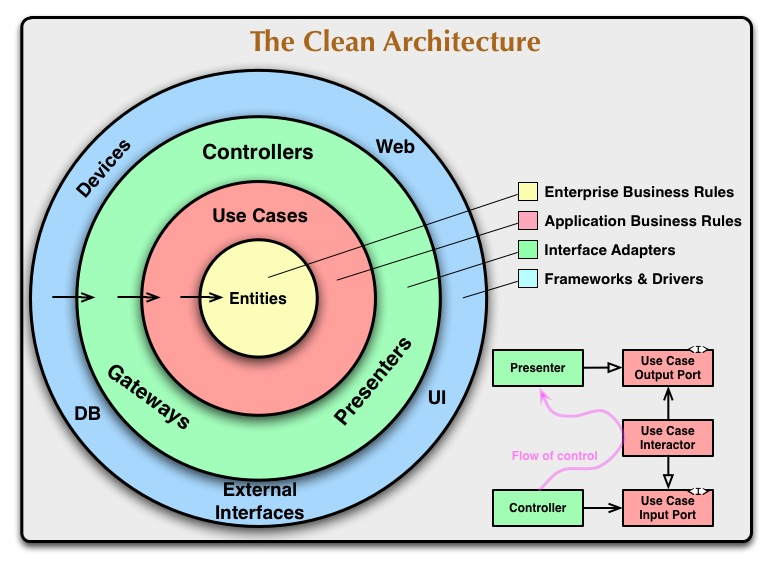
\includegraphics[width=0.8\linewidth]{Images/clean.png}
    \vspace{1em}
    \caption{Minh hoạ Clean Architecture, nguồn \cite{clean}}
    \label{fig:clean}
\end{figure}

Ở mức độ chi tiết, Thực thể đóng vai trò như những yếu tố cơ bản trong kiến trúc, đóng gói quy tắc kinh doanh toàn diện. Dù có dạng đối tượng hoặc là cấu trúc dữ liệu và chức năng, thực thể không quan tâm đến ứng dụng cụ thể nào đang sử dụng chúng. Trong khi đó, Lớp Use Cases chứa quy tắc kinh doanh cụ thể cho ứng dụng và đảm bảo luồng dữ liệu giữa các thực thể.\\

Interface Adapters đóng vai trò như trung gian, chuyển đổi dữ liệu giữa định dạng thuận tiện nhất cho Use Cases và Thực thể và định dạng thuận tiện nhất cho đơn vị bên ngoài như cơ sở dữ liệu hoặc web. Cuối cùng, lớp Frameworks và Drivers chứa các công cụ và chi tiết cấp thấp nhất, như cơ sở dữ liệu và framework web, với chức năng chính là đóng vai trò như một đường ống.\\

Quy tắc phụ thuộc luôn được duy trì, giúp tăng cường trừu tượng hóa theo hướng vòng tròn bên trong. Mỗi lớp giữ vai trò của một hộp chứa độc lập, giúp duy trì sự cân bằng giữa linh hoạt và sự kiểm soát trong thiết kế kiến trúc Clean Architecture.

\section{Design pattern: DI and builder}

$\indent$Trong thế giới phát triển phần mềm hiện đại, việc sử dụng Design Pattern không chỉ là một xu hướng mà còn là một chiến lược quan trọng để tạo ra mã nguồn dễ bảo trì và linh hoạt. Hai mô hình quan trọng, Dependency Injection (DI) và Builder Pattern, là những "công cụ" quan trọng trong "hộp công cụ" của các nhà phát triển giúp tối ưu hóa việc quản lý các thành phần của hệ thống và cung cấp khả năng linh hoạt đáng kể trong việc xây dựng đối tượng phức tạp.

\section*{Dependency Injection (DI):}

$\indent$ DI \cite{di} là một design pattern tập trung vào việc giảm sự phụ thuộc giữa các thành phần của hệ thống, giúp tăng tính linh hoạt và kiểm soát. Thay vì các đối tượng tạo ra và quản lý chính nó, DI chuyển trách nhiệm này đến bên ngoài, thường là một hệ thống quản lý phụ thuộc (dependency container). Điều này giúp giảm độ kết dính giữa các thành phần, làm cho mã nguồn dễ bảo trì và mở rộng hơn. Hơn nữa, DI thúc đẩy việc tái sử dụng mã nguồn, vì các đối tượng không phụ thuộc trực tiếp vào cách chúng được tạo ra.

\begin{figure}[h]
    \centering
    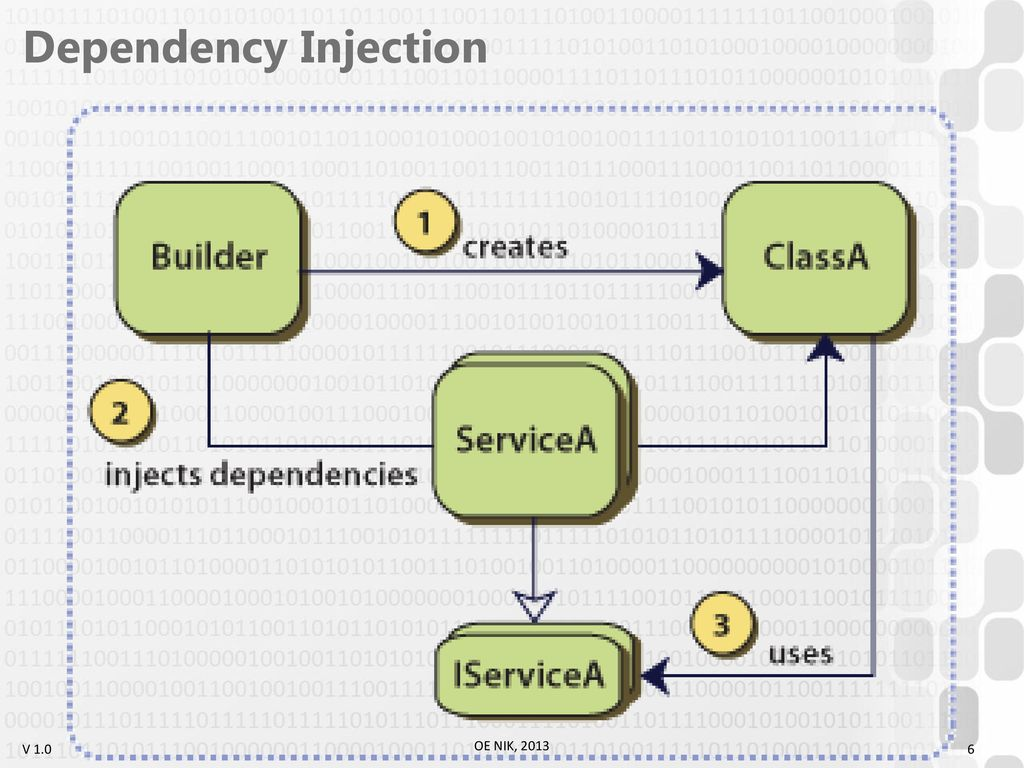
\includegraphics[width=0.6\linewidth]{Images/DI.png}
    \vspace{1em}
    \caption{Dependency Injection}
    
\end{figure}
\newpage
\section*{Builder Pattern:}

$\indent$ Builder Pattern \cite{builder} tập trung vào việc xây dựng đối tượng phức tạp, giúp tách rời quá trình xây dựng và biểu diễn. Thay vì sử dụng nhiều constructor hoặc phương thức khởi tạo, Builder Pattern cung cấp một cách linh hoạt và tự nhiên để xây dựng đối tượng bằng cách sử dụng một builder object. Điều này không chỉ làm cho mã nguồn dễ đọc hơn mà còn giúp quản lý các tham số xây dựng, đặc biệt là khi có nhiều tùy chọn. Builder Pattern thường được sử dụng để xây dựng các đối tượng không thay đổi và không có sự thay đổi trạng thái, giúp giảm lỗi và làm tăng khả năng kiểm thử.

\begin{figure}[h]
    \centering
    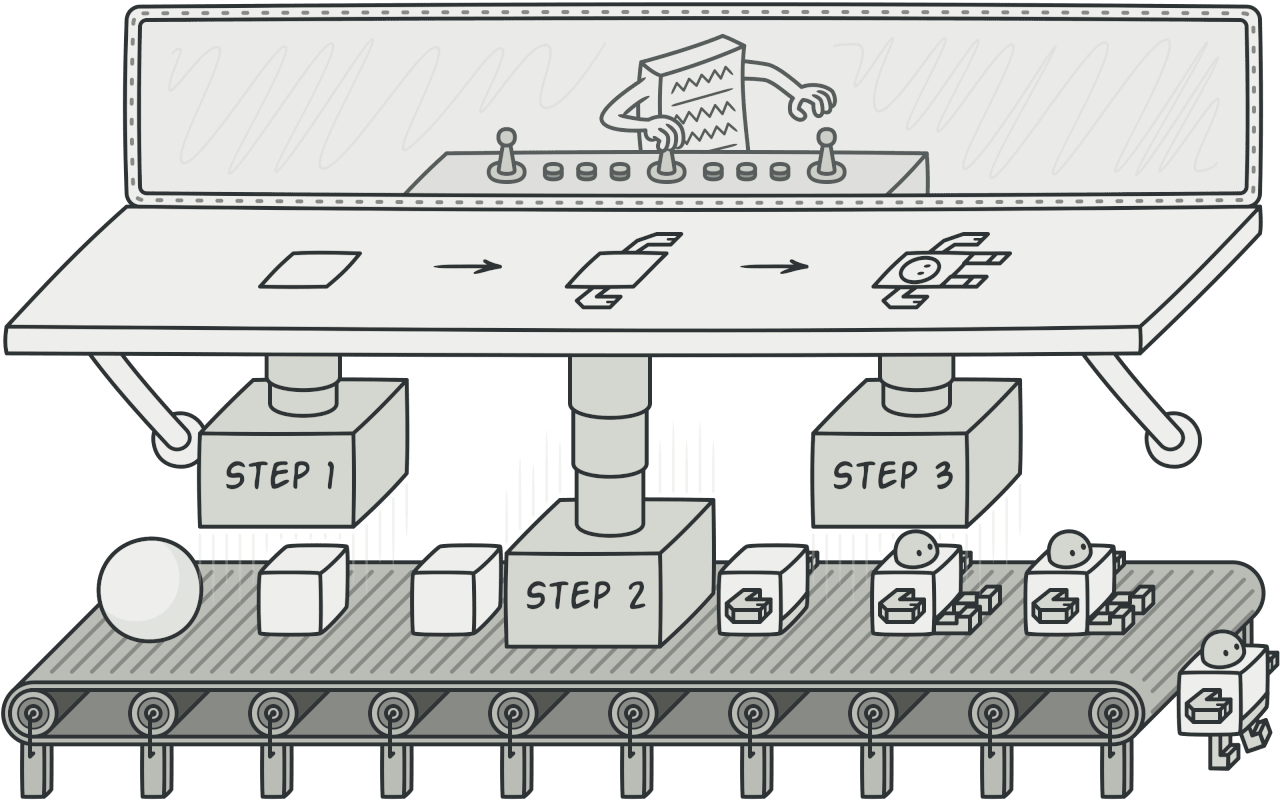
\includegraphics[width=\linewidth]{Images/builder.png}
    \vspace{1em}
    \caption{Builder cho phép xây dựng các đối tượng phức tạp theo từng bước}
    
\end{figure}

\section*{Tích Hợp DI và Builder Pattern:}

$\indent$ Khi kết hợp DI và Builder Pattern, chúng ta có thể tận dụng sức mạnh của cả hai mô hình để tạo ra hệ thống linh hoạt, dễ bảo trì, và có thể mở rộng một cách dễ dàng. Dependency Injection giảm sự phụ thuộc, trong khi Builder Pattern giúp quản lý quá trình xây dựng các đối tượng phức tạp. Sự kết hợp này làm cho mã nguồn dễ đọc, dễ kiểm thử, và giảm thiểu các vấn đề liên quan đến thiết kế và xây dựng.\\

Bằng cách tận dụng sự mạnh mẽ của cả Dependency Injection và Builder Pattern, chúng ta có thể xây dựng các hệ thống linh hoạt và dễ bảo trì, đồng thời giảm thiểu rủi ro về lỗi và tăng tính mở rộng của mã nguồn.

\section{Front-end}
\subsection{Next.js với TypeScript}
$\indent$ Next.js \cite{nextjs} là một framework React mã nguồn mở được phát triển bởi Vercel, nhằm cung cấp một giải pháp toàn diện cho việc xây dựng ứng dụng web hiện đại. Next.js kế thừa tất cả ưu điểm của React và bổ sung thêm nhiều tính năng mạnh mẽ. 

Next.js sử dụng cách tiếp cận "page-based routing" kết hợp với "component-based" của React để xây dựng giao diện. Điều này cho phép tổ chức cấu trúc ứng dụng một cách trực quan và hiệu quả, đồng thời vẫn giữ được khả năng tái sử dụng và modular hóa cao của các component. Cách tiếp cận này giúp tách biệt logic và giao diện, dễ dàng quản lý và bảo trì mã nguồn, đồng thời tạo ra một kiến trúc ứng dụng rõ ràng và dễ mở rộng.

Một trong những tính năng nổi bật của Next.js là khả năng Server-Side Rendering (SSR) và Static Site Generation (SSG). SSR giúp cải thiện đáng kể thời gian tải trang đầu tiên và tối ưu hóa SEO, trong khi SSG cho phép tạo ra các trang tĩnh tại thời điểm build, giúp tăng tốc độ và giảm tải cho server. Next.js cũng hỗ trợ Incremental Static Regeneration (ISR), cho phép cập nhật từng phần của trang tĩnh mà không cần phải build lại toàn bộ site \cite{nextjs-features}.

Next.js tích hợp sẵn nhiều tính năng quan trọng như code splitting, lazy loading, và tối ưu hóa hình ảnh. Điều này giúp cải thiện hiệu suất ứng dụng một cách đáng kể mà không cần cấu hình phức tạp.

Khi kết hợp Next.js với TypeScript, ta có thể tận dụng tất cả lợi ích của việc kiểm tra kiểu tĩnh và lập trình hướng đối tượng mạnh mẽ. TypeScript giúp phát hiện lỗi trong quá trình biên dịch và cung cấp các tính năng gỡ lỗi thông minh, tăng tính ổn định và độ tin cậy của ứng dụng \cite{typescript}.

Việc sử dụng TypeScript với Next.js còn mang lại lợi ích trong việc quản lý trạng thái và props của components. TypeScript cho phép xác định các kiểu dữ liệu chính xác cho trạng thái, props, và các API routes của Next.js, giúp tạo ra mã nguồn dễ đọc, dễ hiểu và dễ bảo trì. Điều này đặc biệt hữu ích trong các dự án lớn và phức tạp.

Next.js cũng cung cấp API Routes, cho phép xây dựng API serverless một cách dễ dàng. Kết hợp với TypeScript, ta có thể tạo ra các API an toàn về kiểu dữ liệu và dễ dàng tích hợp với phần front-end của ứng dụng.

Tóm lại, Next.js kết hợp với TypeScript là một công cụ mạnh mẽ cho phát triển ứng dụng web hiện đại. Với khả năng SSR, SSG, ISR, hiệu suất cao, kiến trúc dựa trên pages và components, tính năng mạnh mẽ của TypeScript và sự hỗ trợ từ cộng đồng, Next.js giúp tạo ra các ứng dụng web linh hoạt, có hiệu suất cao, dễ bảo trì và đáng tin cậy.

\begin{figure}[h]
    \centering
    
\includegraphics[width=0.5\linewidth]{Images/nextjs.png}
    \vspace{1em}
    \caption{Next.js và Typescript}
    
\end{figure}
\newpage
\subsection{Mantine}
$\indent$ Mantine \cite{mantine} là một thư viện UI React mã nguồn mở, cung cấp các thành phần giao diện đẹp mắt, dễ sử dụng và linh hoạt. Nó cung cấp một tập hợp các thành phần giao diện hiện đại, từ các nút, biểu mẫu và bảng cho đến các thanh trượt, menu và hộp thoại. Điều này giúp tạo ra giao diện thân thiện với người dùng, hiệu quả và đồng nhất trên toàn bộ ứng dụng.\\

Một trong những điểm mạnh của Mantine là tính tùy chỉnh cao. Nó không chỉ cung cấp các thành phần giao diện sẵn có, mà còn cho phép người phát triển tùy chỉnh chúng dựa trên nhu cầu cụ thể. Điều này đảm bảo rằng giao diện cuối cùng sẽ phù hợp với mục tiêu thiết kế và mong muốn của người dùng.\\

Ngoài ra, Mantine còn cung cấp một bộ tài liệu phong phú và chi tiết, gồm hướng dẫn sử dụng, ví dụ mẫu và hướng dẫn thiết kế. Điều này giúp người phát triển nhanh chóng làm quen với Ant Design và tận dụng tối đa các tính năng mạnh mẽ của nó.\\

Mantine là một lựa chọn lý tưởng để xây dựng giao diện người dùng chất lượng và dễ sử dụng trong các dự án phát triển phần mềm. Với tính tương thích, tích hợp dễ dàng, tính tùy chỉnh cao, Mantine là lựa chọn thích hợp đối với công cụ phát triển giao diện người dùng.

\begin{figure}[h]
    \centering
    
\includegraphics[width=0.5\linewidth]{Images/matine.png}
    \vspace{1em}
    \caption{Mantine}
    
\end{figure}

\subsection{Vercel}
$\indent$ Vercel \cite{vercel} là một nền tảng triển khai và lưu trữ trang web, ứng dụng Front-end được phát triển bởi Vercel, Inc. (trước đây là Zeit). Nền tảng này được thiết kế đặc biệt để triển khai các ứng dụng web hiện đại và tĩnh dựa trên các framework như React, Next.js, Vue.js và Nuxt.js.\\

Với Vercel, có thể dễ dàng triển khai mã nguồn thông qua quy trình CI/CD tích hợp sẵn. Nền tảng này tự động xây dựng, triển khai và cung cấp các bản xem trước cho mỗi lần push code lên Git. Vercel cũng cung cấp các tính năng như phân phối nội dung toàn cầu thông qua mạng CDN, quản lý các bản triển khai, tích hợp các dịch vụ bên thứ ba và tự động hóa quy trình build/deploy.\\

Một trong những lợi ích chính của Vercel là nó cho phép tập trung vào việc xây dựng ứng dụng mà không cần phải lo lắng về việc quản lý cơ sở hạ tầng triển khai. Vercel xử lý tất cả các nhiệm vụ liên quan đến triển khai, bảo mật và mở rộng, giúp gia tăng năng suất và tập trung vào phát triển tính năng.
\begin{figure}[h]
    \centering
    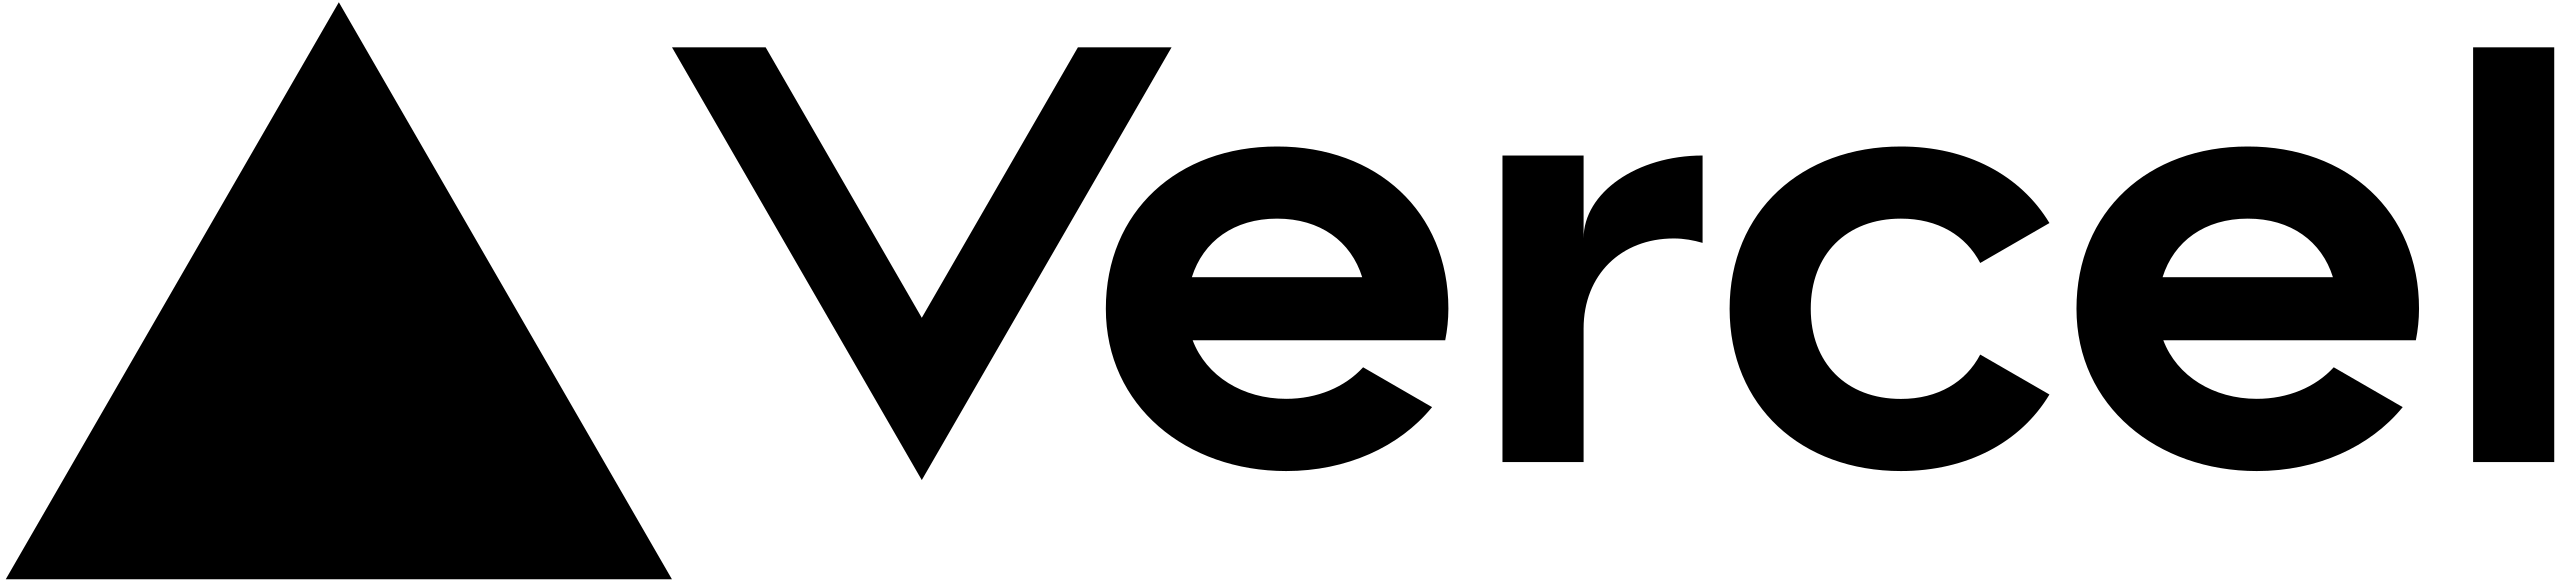
\includegraphics[width=0.5\linewidth]{Images/vercel.png}
    \vspace{1em}
    \caption{Vercel}
\end{figure}
\section{Back-end - Database}
\subsection{ASP.NET Core và Entity Framework (EF) Core}

$\indent$ ASP.NET Core \cite{asp}là một framework phát triển ứng dụng web mạnh mẽ được phát triển bởi Microsoft. Nó cung cấp một nền tảng cho việc xây dựng các ứng dụng web đa dạng và mạnh mẽ bằng cách sử dụng ngôn ngữ lập trình C\#.\\

Entity Framework(EF) Core là một ORM (Object-Relational Mapping) framework cũng do Microsoft phát triển, giúp tương tác và quản lý cơ sở dữ liệu trong ứng dụng. Nó giúp lập trình viên làm việc với dữ liệu cơ sở dữ liệu bằng cách sử dụng đối tượng và cung cấp một lớp trừu tượng giúp ẩn đi các chi tiết về cơ sở dữ liệu thực tế.\\ 

Khi kết hợp sử dụng ASP.NET Core và Entity Framework Core, người phát triển có thể xây dựng các ứng dụng web mạnh mẽ và dễ dàng quản lý cơ sở dữ liệu. Thông qua Entity Framework Core, dữ liệu được quản lý trong các đối tượng .NET, giúp giảm thiểu việc phải viết các câu truy vấn SQL trực tiếp. Thêm vào đó, ASP.NET Core cung cấp nền tảng cho việc xây dựng các giao diện người dùng tương tác, cho phép người dùng tương tác với dữ liệu được quản lý bởi Entity Framework Core.\\

Tóm lại, sự kết hợp giữa ASP.NET Core và Entity Framework Core cung cấp cho các nhà phát triển một cách tiếp cận toàn diện để xây dựng ứng dụng web chất lượng cao với khả năng tương tác với dữ liệu hiệu quả.

\begin{figure}[H]
    \centering
    
\includegraphics[width=0.55\linewidth]{Images/asp-ef.png}
    \vspace{1em}
    \caption{EF Core và ASP.NET Core}
    
\end{figure}


\subsection{PostgreSQL Database}
$\indent$ PostgreSQL Database \cite{postgreSql} là một hệ quản trị cơ sở dữ liệu quan hệ mã nguồn mở mạnh mẽ và đáng tin cậy, được phát triển bởi cộng đồng PostgreSQL Global Development Group. Với hơn 30 năm phát triển, PostgreSQL đã trở thành một trong những lựa chọn hàng đầu cho các ứng dụng yêu cầu độ tin cậy cao, tính toàn vẹn dữ liệu, và khả năng xử lý khối lượng lớn.

Dự án đã tận dụng sức mạnh của PostgreSQL thông qua dịch vụ Neon, một nền tảng cung cấp PostgreSQL trên cloud. Neon cung cấp một giải pháp serverless, cho phép tập trung vào việc phát triển ứng dụng mà không cần lo lắng về việc quản lý cơ sở hạ tầng. Điều này giúp tối ưu hóa chi phí vận hành và tăng tính linh hoạt cho hệ thống.

Tính năng ACID (Atomicity, Consistency, Isolation, Durability) của PostgreSQL đảm bảo tính toàn vẹn dữ liệu cao, điều này đặc biệt quan trọng đối với các ứng dụng yêu cầu độ tin cậy cao như hệ thống của nhóm. Ngoài ra, PostgreSQL còn cung cấp các tính năng nâng cao như partitioning, replication, và full-text search, giúp tối ưu hóa hiệu suất và khả năng mở rộng của hệ thống.

Về mặt bảo mật, PostgreSQL cung cấp nhiều lớp bảo vệ, bao gồm xác thực mạnh mẽ, mã hóa dữ liệu, và kiểm soát truy cập chi tiết. Khi kết hợp với các tính năng bảo mật của Neon, có thể đảm bảo rằng dữ liệu của người dùng luôn được bảo vệ ở mức cao nhất.

PostgreSQL cũng nổi tiếng với khả năng mở rộng và hiệu suất cao. Nó có thể xử lý hàng triệu bản ghi một cách hiệu quả, đồng thời hỗ trợ các truy vấn phức tạp và các giao dịch đồng thời. Điều này cho phép ứng dụng phục vụ số lượng lớn người dùng mà không gặp vấn đề về hiệu suất.

Cuối cùng, việc sử dụng PostgreSQL trên nền tảng Neon cho phép tận dụng các tính năng như sao lưu tự động, khôi phục điểm thời gian, và scaling tự động. Điều này giúp đảm bảo tính khả dụng cao và khả năng phục hồi nhanh chóng trong trường hợp xảy ra sự cố.

Tóm lại, việc lựa chọn PostgreSQL trên nền tảng Neon đã cung cấp một giải pháp cơ sở dữ liệu mạnh mẽ, linh hoạt và đáng tin cậy. Nó không chỉ đáp ứng các yêu cầu hiện tại của dự án mà còn cung cấp nền tảng vững chắc cho sự phát triển trong tương lai.

\begin{figure}[H]
    \centering
    
\includegraphics[width=0.8\linewidth]{Images/tech_database.png}
    \vspace{1em}
    \caption{PostgreSQL Service}
    
\end{figure}


\chapter{Phân tích hệ thống}
    \label{chap:phan-tich-nghiep-vu}
    \section{Phân tích nghiệp vụ chức năng người dùng}
    \subsection{Chủ cửa hàng}
        \subsubsection{Nghiệp vụ quản lý cửa hàng}
        \begin{enumerate}
            \item Tạo cửa hàng: Doanh nghiệp hoặc cá nhân cần tạo cửa hàng trên tài khoản của mình tại trang web thương mại điện tử để bắt đầu kinh doanh.
            \item Tạo sản phẩm bán: Cửa hàng cần tạo sản phẩm và cung cấp đầy đủ thông tin về sản phẩm, bao gồm tên sản phẩm, mô tả sản phẩm, giá cả, hình ảnh, và thông tin vận chuyển.
            \item Thêm số lượng sẵn có: Cửa hàng cần cập nhật số lượng sản phẩm sẵn có để khách hàng có thể biết được sản phẩm còn hàng hay đã hết hàng.
            \item Thêm mô tả cho sản phẩm: Mô tả sản phẩm là một yếu tố quan trọng giúp khách hàng hiểu rõ về sản phẩm. Cửa hàng cần cung cấp mô tả sản phẩm đầy đủ và chi tiết.
            \item Tạo các danh mục sản phẩm: Danh mục sản phẩm giúp khách hàng dễ dàng tìm kiếm sản phẩm. Cửa hàng nên tạo các danh mục sản phẩm rõ ràng và logic để giúp khách hàng tìm kiếm sản phẩm dễ dàng hơn.
            \item Điều chỉnh giá thành của sản phẩm: Giá thành của sản phẩm là một yếu tố quan trọng ảnh hưởng đến quyết định mua hàng của khách hàng. Cửa hàng nên điều chỉnh giá thành của sản phẩm phù hợp với thị trường để tăng doanh số bán hàng.
            \item Tạo các combo sản phẩm: Combo sản phẩm là một cách hiệu quả để tăng giá trị cho khách hàng. Cửa hàng có thể tạo các combo sản phẩm với giá ưu đãi để thu hút khách hàng mua nhiều sản phẩm hơn.
            \item Thêm các chương trình tặng quà khi mua sản phẩm: Các chương trình tăng quà khi mua sản phẩm là một cách hiệu quả để khuyến khích khách hàng mua hàng. Của hàng có thể tạo các chương trình tăng quà khi mua sản phẩm để thu hút khách hàng mới và tăng doanh số bán hàng cho các sản phẩm bán chạy.
        \end{enumerate}
        \subsubsection{Nghiệp vụ quản lý sản phẩm}
        $\indent$ Nghiệp vụ sản phẩm trên sàn thương mại điện tử nông sản bao gồm quá trình quản lý và tiếp thị sản phẩm để thu hút khách hàng, tạo ra doanh số bán hàng, và đảm bảo sự hài lòng của khách hàng. Quản lý sản phẩm trên sàn thương mại điện tử nông sản là một phần quan trọng của hoạt động kinh doanh và đòi hỏi sự chú ý đến chi tiết, hiểu biết về thị trường và nhu cầu của khách hàng, cũng như khả năng tiếp tục tối ưu hóa sản phẩm và chiến dịch tiếp thị.
        \begin{enumerate}
            \item Quản lý Sản Phẩm:
        
        - Thêm, chỉnh sửa, và xóa sản phẩm trên sàn thương mại điện tử.
        
        - Cung cấp thông tin chi tiết về sản phẩm, bao gồm tên, mô tả, hình ảnh, giá cả, số lượng tồn kho, và các thuộc tính kèm theo.
            \item Phân Loại Sản Phẩm:
        Tạo danh mục và phân loại sản phẩm để giúp khách hàng dễ dàng tìm kiếm và duyệt qua các sản phẩm tương tự.
            \item Thông Tin sản phẩm:
        Cung cấp thông tin chi tiết về sản phẩm, ví dụ như trọng lượng, kích thước, xuất xứ, thời hạn sử dụng, và hướng dẫn sử dụng.
            \item Giá và Chiết Khấu:
        - Xác định giá cả cho sản phẩm, bao gồm giá gốc và giá bán.
        
        - Áp dụng chiết khấu hoặc ưu đãi đặc biệt nếu có.
            \item Quản lý Tồn Kho:
        Theo dõi số lượng tồn kho của từng sản phẩm và cập nhật thông tin về số lượng sản phẩm còn lại tức thì.
            \item Quản lý Đánh Giá và Nhận Xét:
        
        - Cho phép khách hàng đánh giá và viết nhận xét về sản phẩm.
        
        - Kiểm duyệt và quản lý đánh giá và nhận xét để đảm bảo tính trung thực và hữu ích.
            \item Quản lý Sản Phẩm Liên Quan:
        Kết nối các sản phẩm tương tự hoặc có liên quan để thúc đẩy giao dịch chéo (cross-selling) và gợi ý sản phẩm.
            \item Tối ưu hóa Sản Phẩm:
        Sản phẩm nên được cập nhật đều đặn để cải thiện tính năng, chất lượng, hoặc cách sử dụng để đáp ứng nhu cầu khách hàng ngày càng biến đổi.
            \item Chăm sóc và Hỗ trợ Sản Phẩm:
        Cung cấp hỗ trợ kỹ thuật, chăm sóc sau bán hàng, và hướng dẫn sử dụng sản phẩm cho khách hàng.
            \item Quản lý Sản Phẩm Bán Chạy và Lưu Lượng:
        Theo dõi sản phẩm nào đang bán chạy và đảm bảo rằng sản phẩm luôn có sẵn trong kho để đáp ứng nhu cầu.
        \end{enumerate}
        
        \subsubsection{Nghiệp vụ bán hàng}
        \begin{enumerate}
            \item Xác nhận đơn hàng:
        
        - Người bán xác nhận đơn hàng và chuẩn bị sản phẩm cho quá trình giao hàng.
        
        - Hệ thống gửi thông báo xác nhận đơn hàng đến người mua.
            \item Giao hàng:
        
        - Người bán chọn phương thức vận chuyển và gửi sản phẩm đến địa chỉ giao hàng được xác định trong đơn hàng.
        
        - Hệ thống cung cấp thông tin vận chuyển để người mua có thể theo dõi quá trình vận chuyển.
        \item  Nhận và kiểm tra sản phẩm:
        
        - Người mua nhận sản phẩm và kiểm tra tính chất và chất lượng của sản phẩm.
        
        - Họ có thể đánh giá sản phẩm sau khi nhận hàng.
            \item Hỗ trợ khách hàng sau bán hàng:
        Sàn thương mại điện tử cung cấp dịch vụ hỗ trợ khách hàng sau bán hàng để giải quyết mọi thắc mắc hoặc khiếu nại của người mua.
            \item Theo dõi lịch sử đơn hàng:
        Hệ thống lưu trữ lịch sử đơn hàng của người mua và người bán, giúp họ theo dõi trạng thái và thông tin chi tiết về đơn hàng trước đây.
            \item Đánh giá và đánh giá sản phẩm:
        Sau khi nhận sản phẩm, người mua có thể đánh giá và viết nhận xét về sản phẩm và dịch vụ của người bán để cung cấp phản hồi cho cộng đồng mua sắm trực tuyến.
        \end{enumerate}
        
        \subsubsection{Nghiệp vụ hỗ trợ khách hàng}
	\begin{enumerate}
            \item Hướng Dẫn Sử Dụng Sản Phẩm:
        Cung cấp hướng dẫn sử dụng chi tiết cho sản phẩm để giúp khách hàng tận dụng tối đa sản phẩm mà họ đã mua.
		\item Xử Lý Phản Hồi Khách Hàng:
        Lắng nghe phản hồi từ khách hàng để cải thiện dịch vụ và sản phẩm.
            \item Trả lời Câu hỏi và Thắc mắc:
        Hỗ trợ người mua trả lời câu hỏi và giải đáp thắc mắc liên quan đến sản phẩm, cách sử dụng, vận chuyển, và chính sách đổi trả.
            \item Phản hồi và Đánh giá:
        Thu thập phản hồi và đánh giá từ người mua để cải thiện chất lượng sản phẩm và dịch vụ.
            \item Chăm sóc Khách hàng Sau Bán hàng:
        Cung cấp dịch vụ chăm sóc khách hàng sau bán hàng để đảm bảo họ hài lòng với sản phẩm và dịch vụ.
	\end{enumerate}
 
        \subsubsection{Quản lý ưu đãi}
        Nghiệp vụ ưu đãi và khuyến mãi trên sàn thương mại điện tử nông sản đóng một vai trò quan trọng trong việc thu hút khách hàng, tạo động lực mua sắm, và tăng doanh số bán hàng. Dưới đây là một số chi tiết về nghiệp vụ này:
        
        \begin{enumerate}
            \item Tạo Chương Trình Khuyến Mãi:
        
        - Xác định mục tiêu và đối tượng của chương trình khuyến mãi (Ví dụ: giảm giá sản phẩm nông sản trong mùa thu).
        
        - Quyết định loại ưu đãi, chẳng hạn như giảm giá tiền mặt, vận chuyển miễn phí, quà tặng kèm, hoặc voucher.
            \item Xác định Điều Kiện Áp Dụng:
        Quy định điều kiện và hạn chế áp dụng cho ưu đãi, bao gồm thời gian, số lượng, loại sản phẩm, và quy định về sử dụng.
            \item Quản Lý Mã Giảm Giá Và Voucher:
        
        - Tạo và quản lý các mã giảm giá và voucher để phân phối cho khách hàng.
        
        - Theo dõi và kiểm soát việc sử dụng mã giảm giá để đảm bảo tính hợp lệ và tuân thủ các quy định.
            \item Quảng Cáo Khuyến Mãi:
        
        - Tạo chiến dịch quảng cáo để thông báo về chương trình khuyến mãi.
        
        - Sử dụng các kênh quảng cáo trực tuyến như quảng cáo trên mạng xã hội, email marketing, và quảng cáo trực tuyến để tiếp cận khách hàng.
            \item Theo Dõi Hiệu Suất:
        Theo dõi hiệu suất chương trình khuyến mãi bằng cách thu thập dữ liệu về số lượng sử dụng, doanh số bán hàng tăng, và ROI (Return on Investment).
            \item Lập Kế Hoạch Và Thời Gian:
        
        - Xác định lịch trình khuyến mãi, bao gồm thời gian bắt đầu và kết thúc của chương trình.
        
        - Đảm bảo rằng sản phẩm và dịch vụ có sẵn trong kho để đáp ứng nhu cầu.
            \item Hỗ trợ Khách Hàng:
        Cung cấp hỗ trợ cho khách hàng liên quan đến chương trình khuyến mãi, bao gồm hướng dẫn sử dụng mã giảm giá và giải quyết khiếu nại.
            
        \end{enumerate}
        
        \subsubsection{Quản lý đánh giá}
        \begin{enumerate}
            \item Tạo khuyến mãi dựa trên đánh giá: Sử dụng đánh giá tích cực để tạo chương trình khuyến mãi và đánh giá sản phẩm nổi bật.
            \item  Theo Dõi Phản Hồi Của Khách Hàng:
        Theo dõi phản hồi từ khách hàng về sản phẩm và dịch vụ để cải thiện chất lượng và trải nghiệm của họ.
            \item Quản Lý Đánh Giá Gắn Kèm Hình Ảnh:
        Cho phép khách hàng đính kèm hình ảnh và video vào đánh giá sản phẩm.
            \item Hiển Thị Đánh Giá Trên Trang Sản Phẩm:
        Đánh giá và đánh giá sản phẩm thường được hiển thị trên trang sản phẩm để giúp người mua xem được đánh giá sản phẩm trước khi mua.
            \item Phản Hồi Đánh Giá:
        Cho phép người bán hoặc quản trị viên trả lời các đánh giá để giải quyết các vấn đề hoặc cung cấp thông tin bổ sung.
            \item Hiển Thị Đánh Giá Gắn Kèm Hình Ảnh:
        Cho phép khách hàng đính kèm hình ảnh hoặc video vào đánh giá sản phẩm để cung cấp thêm thông tin.
            \item Đánh Giá Về Dịch Vụ Giao Hàng:
        Cho phép khách hàng đánh giá dịch vụ giao hàng, bao gồm thời gian giao hàng và tình trạng sản phẩm khi nhận hàng.
            \item Tạo Bài Viết Đánh Giá Tương Tác:
        Cho phép người dùng tương tác với các đánh giá bằng cách bình luận hoặc bỏ phiếu cho những đánh giá có ích.
        \end{enumerate}
        \subsubsection{Nghiệp vụ quản lý hậu thu hoạch}
        Nghiệp vụ quản lý hậu thu hoạch kết hợp với logistics giúp tối ưu hóa các hoạt động sau thu hoạch, bao gồm bảo quản, vận chuyển nông sản. Trên hệ thống, chủ cửa hàng có thể theo dõi chi tiết thông tin sản phẩm như chất lượng, số lượng, thời gian thu hoạch. Họ cũng quản lý các hoạt động logistics như lập lịch trình vận chuyển, theo dõi tình trạng giao hàng theo thời gian thực. Hệ thống còn giúp giám sát tình trạng kho bãi, cảnh báo khi sản phẩm sắp hết hạn sử dụng. 
        \begin{enumerate}
            \item Quản lý thông tin sản phẩm:\\
                - Theo dõi thông tin chi tiết về từng loại sản phẩm như tên, số lượng, chất lượng, thời gian thu hoạch.\\
                - Phân loại, đánh mã định danh cho từng lô hàng.\\
                - Cập nhật tình trạng sản phẩm trong các giai đoạn bảo quản, vận chuyển.\\
            \item Quản lý hoạt động logistics:\\
                - Lập kế hoạch và theo dõi lịch trình vận chuyển, bao gồm phương tiện, tuyến đường, thời gian giao hàng.\\
                - Theo dõi tình trạng vận chuyển theo thời gian thực, như vị trí hiện tại của các lô hàng.\\
            \item Quản lý kho bãi:\\
                - Theo dõi tình trạng kho, như nhiệt độ, độ ẩm, diện tích kho trống.\\
                - Quản lý việc nhập, xuất, tồn kho các lô sản phẩm.\\
                - Cảnh báo khi sản phẩm sắp hết hạn sử dụng hoặc cần phải xử lý.\\
        \end{enumerate}

        \subsubsection{Quản lý đơn đặt trước}
        Đối với một số sản phẩm nông sản, không thể sản xuất hàng loạt và bảo quản lâu dài, cũng như một số sản phẩm chưa đến mùa vụ thì không thể đưa lên sàn bán được. Khi đó, khách hàng có thể tiến hành đặt trước các sản phẩm này và được giao ngay sau khi có hàng. Nghiệp vụ quản lý đơn đặt trước là một trong những hoạt động quan trọng, nó giúp chủ cửa hàng tiếp nhận, xử lý và quản lý các đơn đặt hàng từ khách hàng một cách hiệu quả. Nghiệp vụ này kết hợp chặt chẽ với công tác logistics để đảm bảo hàng hóa được giao đúng thời gian và địa điểm.

        Đa số các hoạt động trong nghiệp vụ này đều giống nghiệp vụ bán hàng, chẳng hạn như tiếp nhận đơn đặt hàng, cập nhật tình trạng đơn, quản lý kho hàng, v.v. đều được thực hiện trên hệ thống của cửa hàng. Tuy nhiên có một số hoạt động cần phải cập nhật thêm các vấn đề liên quan tới tình trạng thu hoạch, sản xuất sản phẩm và thời gian giao hàng.
        \begin{enumerate}
            \item Tiếp nhận đơn đặt trước từ khách hàng: Cửa hàng tiếp nhận đặt trước các sản phẩm nông sản chưa có sẵn, xác nhận các thông tin như tên sản phẩm, số lượng, thời gian giao hàng mong muốn, thông tin liên hệ khách hàng, và xác nhận lại về thời gian giao hàng dự kiến.
            \item Xác nhận khả năng cung ứng: Chủ cửa hàng kiểm tra kế hoạch sản xuất, thu hoạch để đảm bảo có đủ sản phẩm để đáp ứng yêu cầu của khách hàng.Sau đó sẽ xác nhận với khách hàng về khả năng cung ứng.
            \item Theo dõi quá trình sản xuất, thu hoạch: Theo dõi tiến độ sản xuất, thu hoạch để đảm bảo đủ số lượng sản phẩm cho đơn hàng và cập nhật thông tin cho khách hàng về tiến độ và dự kiến thời gian giao hàng.
            \item Quản lý và cập nhật tình trạng đơn đặt trước:\\
                - Xem và quản lý danh sách các đơn đặt hàng từ khách hàng. Xác nhận khả năng cung cấp sản phẩm theo số lượng và thời gian giao hàng yêu cầu.\\
                - Cập nhật tình trạng đơn hàng (đang chờ thu hoạch, đang vận chuyển, đã giao) vào hệ thống.\\
                - Thông báo định kỳ cho khách hàng về tình trạng đơn hàng của họ.
            \item Quản lý giao nhận:Lên lịch giao hàng cho từng đơn đặt hàng, đảm bảo giao đúng thời gian và xử lý các vấn đề phát sinh trong quá trình giao hàng.\\

        \end{enumerate}
    \newpage    
    \subsection{Khách hàng}
        \subsubsection{Mua hàng}
        \begin{enumerate}
            \item Tìm Kiếm Sản Phẩm:
        Người mua truy cập sàn thương mại điện tử và tìm kiếm sản phẩm nông sản theo nhu cầu và sở thích cá nhân.
            \item Duyệt Danh Mục Sản Phẩm:
        Khám phá danh mục sản phẩm, danh mục, và các chế độ lọc để tìm sản phẩm phù hợp.
            \item Xem Thông Tin Sản Phẩm:
        Đọc thông tin chi tiết về sản phẩm, bao gồm hình ảnh, mô tả, giá cả, thuộc tính kỹ thuật, và đánh giá từ người dùng khác.
            \item Thêm Sản Phẩm Vào Giỏ Hàng:
        Chọn sản phẩm và thêm vào giỏ hàng để chuẩn bị cho việc thanh toán.
            \item Kiểm Tra Giỏ Hàng:
        Xem lại danh sách sản phẩm trong giỏ hàng, kiểm tra số lượng và giá cả, và chỉnh sửa nếu cần thiết.
            \item Đặt Hàng:
        Tiến hành đặt hàng bằng cách chọn phương thức thanh toán và giao hàng, nhập thông tin giao hàng, và xác nhận đơn đặt hàng.
            \item Thanh Toán:
        Thực hiện thanh toán bằng cách sử dụng thẻ tín dụng, thẻ ghi nợ, chuyển khoản ngân hàng, hoặc các phương thức thanh toán trực tuyến khác.
            \item Xác Nhận Đơn Hàng:
        Nhận được xác nhận đơn đặt hàng từ sàn thương mại điện tử thông qua email hoặc ứng dụng di động.
            \item Theo Dõi Đơn Hàng:
        Theo dõi trạng thái đơn hàng và thông tin vận chuyển thông qua sàn thương mại điện tử hoặc hệ thống theo dõi đơn hàng trực tuyến.
            \item Nhận Sản Phẩm:
        Nhận sản phẩm nông sản được giao tới địa chỉ giao hàng đã cung cấp và kiểm tra chất lượng và số lượng sản phẩm.
            \item Đánh Giá và Nhận Xét Sản Phẩm:
        Sau khi sử dụng sản phẩm, người mua có thể đánh giá và viết nhận xét về sản phẩm trên sàn thương mại điện tử để chia sẻ thông tin với người dùng khác.
            \item Lưu Trữ Lịch Sử Mua Hàng:
        Sàn thương mại điện tử lưu trữ lịch sử mua hàng của người dùng để thuận tiện cho việc theo dõi và tái đặt hàng trong tương lai.
            \item Hỗ Trợ Khách Hàng:
        Cung cấp hỗ trợ khách hàng liên quan đến quá trình mua hàng, đổi trả, và các câu hỏi khác.
            \item Phí Vận Chuyển và Thuế:
        Trong quá trình đặt hàng, người mua cần kiểm tra các khoản phí vận chuyển và thuế để đảm bảo hiểu rõ giá tổng cộng của đơn hàng.
            \item Phương Thức Thanh Toán:
        Sàn thương mại điện tử nông sản thường cung cấp nhiều phương thức thanh toán khác nhau, bao gồm thẻ tín dụng, thẻ ghi nợ, PayPal, ví điện tử, và chuyển khoản ngân hàng,...
            \item Đánh Giá Tình Trạng Sản Phẩm:
        Trước khi thanh toán, người mua nên kiểm tra kỹ tình trạng sản phẩm để đảm bảo rằng sản phẩm không bị hỏng hoặc thất lạc.
            \item Lựa Chọn Phương Thức Vận Chuyển:
        Người mua có thể chọn phương thức vận chuyển phù hợp với họ, bao gồm giao hàng tận nơi, lấy hàng tại cửa hàng, hoặc vận chuyển ưu đãi.
            \item Theo Dõi Đơn Hàng:
        Cung cấp mã theo dõi để người mua có thể theo dõi trạng thái vận chuyển của đơn hàng và biết khi nào sản phẩm sẽ được giao đến.
            \item An Toàn Thanh Toán:
        Đảm bảo tính an toàn của quá trình thanh toán trực tuyến bằng cách sử dụng các trang web có tích hợp mã hóa và cung cấp hướng dẫn về an toàn thanh toán.
            \item Xử Lý Thanh Toán Hậu Kiểm:
        Người mua nên kiểm tra tài khoản ngân hàng hoặc thẻ tín dụng sau khi thanh toán để xác nhận rằng giao dịch đã được xử lý một cách chính xác.
            \item Hỗ Trợ Trực Tuyến:
        Cung cấp hỗ trợ trực tuyến qua chat trực tiếp, điện thoại hoặc email để giúp người mua giải quyết các vấn đề liên quan đến đơn hàng.
            \item Chương Trình Khách Hàng Thân Thiết:
        Cung cấp các chương trình khách hàng thân thiết và tích điểm để khuyến khích người mua quay lại và mua sắm thường xuyên.
            \item Xác Nhận Giao Dịch:
        Người mua nên nhận được xác nhận giao dịch sau khi hoàn tất việc thanh toán để làm bằng chứng cho đơn hàng của họ.
        \end{enumerate}
        \subsubsection{Đặt trước}
        Như đã nói trên nghiệp vụ Quản lý đơn đặt trước, khách hàng có thể tiến hành đặt trước đối với một số sản phẩm không có sẵn hay các loại nông sản chưa thu hoạch ngay được. Về cơ bản, nghiệp vụ này cũng có các hoạt động giống như nghiệp vụ Mua hàng, chỉ có mốt số điểm khác biệt liên quan đến vấn đề thời gian.
        \begin{enumerate}
            \item Xác định nhu cầu và lựa chọn nhà cung cấp: \\
            - Khách hàng xác định loại sản phẩm nông sản cần mua và thời gian dự kiến nhận hàng.\\
            - Tìm kiếm và lựa chọn các nhà cung cấp uy tín trên hệ thống.
            \item Đặt hàng trước: Khách hàng thực hiện đặt hàng trước sản phẩm mong muốn thông qua tính năng đặt trước trên hệ thống. 
            \item Thỏa thuận các điều khoản: Trên nền tảng, khách hàng và chủ cửa hàng thỏa thuận các điều khoản như giá cả, phương thức thanh toán và thời gian dự kiến giao hàng. Các thông tin này được ghi nhận trong đơn hàng đặt trước.
            \item Theo dõi tiến độ sản xuất và giao hàng: Khách hàng có thể theo dõi tình hình sản xuất, thu hoạch thông qua thông tin cập nhật trên nền tảng.
            \item Nhận hàng và thanh toán: Khách hàng nhận hàng đúng số lượng, chất lượng và thời gian đã thỏa thuận, Kiểm tra sản phẩm và thực hiện thanh toán theo đơn hàng đặt trước.
        \end{enumerate}
        \subsubsection{Giỏ hàng và Đơn hàng}
        \begin{enumerate}
            \item Thêm Sản Phẩm Vào Giỏ Hàng:
        Người mua có thể chọn sản phẩm nông sản và thêm chúng vào giỏ hàng của họ thông qua một nút "Thêm vào giỏ hàng" hoặc biểu tượng tương tự.
        \item Xem Giỏ Hàng:
        Khách hàng có thể xem lại danh sách các sản phẩm đã chọn bằng cách truy cập vào giỏ hàng từ giao diện của họ.
            \item Sửa Sản Phẩm Trong Giỏ Hàng:
        Cho phép người mua thay đổi số lượng sản phẩm hoặc loại bỏ sản phẩm khỏi giỏ hàng nếu họ muốn thay đổi đơn hàng của mình.
            \item Tính Tổng Tiền:
        Hệ thống tự động tính tổng tiền cho toàn bộ đơn hàng bằng cách cộng tất cả các món hàng và tính toán thuế và phí vận chuyển (nếu có).
            \item Sử Dụng Mã Giảm Giá hoặc Voucher:
        Cho phép khách hàng áp dụng mã giảm giá hoặc voucher để nhận được ưu đãi hoặc giảm giá trên tổng giá trị đơn hàng.
            \item Chọn Phương Thức Thanh Toán:
        Khách hàng có thể chọn phương thức thanh toán ưa thích, bao gồm thẻ tín dụng, thẻ ghi nợ, ví điện tử, và chuyển khoản ngân hàng.
            \item Đặt Đơn Hàng:
        Khách hàng cần xác nhận đơn hàng và tiến hành đặt hàng sau khi đã xem xét và chỉnh sửa lại giỏ hàng.
            \item Lưu Giỏ Hàng:
        Cho phép người mua lưu giỏ hàng để hoàn tất đơn hàng sau này hoặc để đánh giá lại danh sách sản phẩm.
            \item Kiểm Tra Số Lượng Còn Trong Kho:
        Hệ thống cần kiểm tra số lượng sản phẩm còn trong kho để đảm bảo rằng sản phẩm có sẵn để bán và không bị thiếu hàng.
            \item Thông Báo Về Sản Phẩm Hết Hạn:
        Thông báo cho người mua nếu có sản phẩm trong giỏ hàng đã hết hàng hoặc không còn sẵn.
            \item Tạo Đơn Hàng Tự Động:
        Sau khi khách hàng đặt hàng thành công, hệ thống tự động tạo một đơn hàng và gửi xác nhận đơn hàng đến khách hàng.
            \item Quản Lý Lịch Sử Giỏ Hàng:
        Lưu trữ lịch sử giỏ hàng của khách hàng để họ có thể xem lại và theo dõi các đơn hàng trước đó.
        \item Hiển Thị Thông Tin Sản Phẩm:
        Cho phép người mua xem thông tin chi tiết về sản phẩm trong giỏ hàng, bao gồm tên sản phẩm, giá, mô tả, và hình ảnh.
            \item Tính Toán Tổng Tiền Chi Phí:
        Tính tổng tiền của các sản phẩm trong giỏ hàng, bao gồm giá sản phẩm, thuế, và phí vận chuyển (nếu có).
            \item Xem Lại Đơn Hàng:
        Khách hàng có thể xem lại đơn hàng để đảm bảo rằng mọi thông tin đều chính xác trước khi hoàn tất thanh toán.
            \item Lưu Trữ Giỏ Hàng Tạm Thời:
        Hệ thống cần lưu trữ giỏ hàng tạm thời để khách hàng có thể tiếp tục mua sắm và quay lại giỏ hàng sau khi đã đăng nhập vào tài khoản của họ.
            \item Xử Lý Mã Giảm Giá hoặc Voucher:
        Cho phép người mua nhập mã giảm giá hoặc voucher để nhận ưu đãi hoặc giảm giá trên tổng giá trị đơn hàng.
            \item Sử Dụng Địa Chỉ Giao Hàng Khác Nhau:
        Cho phép khách hàng sử dụng địa chỉ giao hàng khác với địa chỉ mặc định trong tài khoản của họ nếu cần thiết.
            \item Chọn Phương Thức Thanh Toán Phù Hợp:
        Hệ thống cần hỗ trợ nhiều phương thức thanh toán và hiển thị chúng để người mua có thể chọn phương thức thuận tiện nhất.
            \item Tạo Một Đơn Đặt Hàng Chính Thức:
        Khi khách hàng hoàn tất quá trình xem giỏ hàng và chọn phương thức thanh toán, hệ thống tạo một đơn đặt hàng chính thức.
            \item Xác Nhận Đơn Hàng:
        Hệ thống gửi xác nhận đơn hàng đến khách hàng qua email hoặc thông báo trên trang web để thông báo rằng giao dịch đã thành công.
            \item Theo Dõi Trạng Thái Đơn Hàng:
        Cung cấp cho khách hàng khả năng theo dõi trạng thái đơn hàng, từ khi đặt hàng cho đến khi sản phẩm được giao đến.
            \item Hỗ Trợ Thanh Toán An Toàn:
        Đảm bảo tính an toàn của quá trình thanh toán bằng cách sử dụng kỹ thuật mã hóa và các biện pháp bảo mật khác.
            \item Phát Triển Hệ Thống Giỏ Hàng Thân Thiết:
        Phát triển tính năng giỏ hàng thân thiết để lưu trữ thông tin giỏ hàng của khách hàng và tạo trải nghiệm mua sắm liền mạch trên nhiều thiết bị.
            \item Tích Hợp Hệ Thống Thanh Toán Bên Ngoài:
        Tích hợp với cổng thanh toán bên ngoài như PayPal, Stripe, hoặc các dịch vụ thanh toán trực tuyến khác để xử lý thanh toán.
        \end{enumerate}

        \subsubsection{Nghiệp vụ thanh toán}
        \begin{enumerate}
            \item Lựa Chọn Phương Thức Thanh Toán:
        Cho phép khách hàng chọn phương thức thanh toán, bao gồm thẻ tín dụng, thẻ ghi nợ, ví điện tử, chuyển khoản ngân hàng, hoặc các phương thức thanh toán trực tuyến khác.
            \item Nhập Thông Tin Thanh Toán:
        Khách hàng cần cung cấp thông tin thanh toán, bao gồm số thẻ, ngày hết hạn, mã bảo mật, và thông tin liên quan để thực hiện thanh toán.
            \item Xác Thực Thanh Toán:
        Hệ thống cần thực hiện xác thực thông tin thanh toán để đảm bảo tính xác thực và bảo mật giao dịch.
            \item Ghi Nhận Giao Dịch:
        Ghi nhận thông tin giao dịch, bao gồm số tiền, sản phẩm hoặc dịch vụ mua sắm, và thông tin liên quan về giao dịch.
            \item Phân Loại Giao Dịch:
        Phân loại giao dịch thành các loại khác nhau, ví dụ như thanh toán cho đơn hàng, đặt cọc, hoàn tiền, và các loại giao dịch tài chính khác.
            \item Xử Lý Thanh Toán:
        Gửi thông tin thanh toán đến cơ quan xử lý thanh toán hoặc cổng thanh toán để thực hiện giao dịch tài chính.
            \item Theo Dõi Trạng Thái Thanh Toán:
        Theo dõi trạng thái thanh toán để biết khi nào giao dịch đã hoàn thành và tiền đã được chuyển đến tài khoản người bán.
            \item Xác Nhận Thanh Toán:
        Gửi xác nhận thanh toán đến khách hàng để thông báo rằng giao dịch đã thành công.
            \item Bảo Mật Thanh Toán:
        Đảm bảo tính an toàn và bảo mật thông tin thanh toán bằng cách sử dụng mã hóa và các biện pháp bảo mật khác.
            \item Phí Vận Chuyển và Thuế:
        Tính toán và cộng thêm phí vận chuyển và thuế vào tổng số tiền thanh toán nếu áp dụng.
            \item Lưu Trữ Lịch Sử Thanh Toán:
        Lưu trữ lịch sử các giao dịch thanh toán và cung cấp cho khách hàng truy cập vào lịch sử thanh toán của họ.
            \item Phát Triển Chính Sách Thanh Toán:
        Xây dựng và quản lý chính sách liên quan đến thanh toán, bao gồm chính sách đổi trả và hoàn tiền.
        \end{enumerate}
   
    \section{Usecase diagram và đặc tả use-case}
        \subsection{Usecase hệ thống}
            \begin{figure}[H]
                \centering
                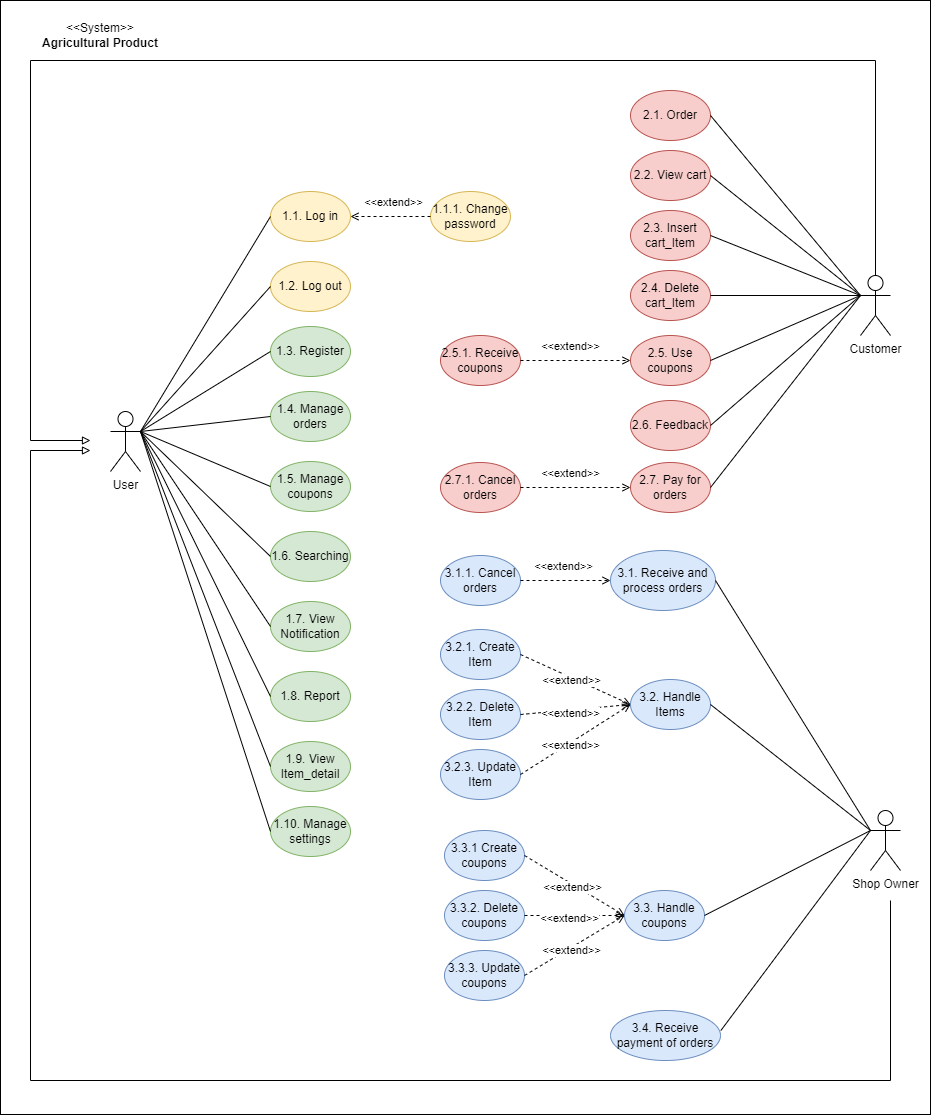
\includegraphics[width=0.5\linewidth]{Images/usecase.png}
                \vspace{1em}
                \caption{Use-case hệ thống}
            \end{figure}
        \newpage
        \subsection{Đặc tả usecase}
            \subsubsection{Đăng nhập}
            \begin{usecase_table}[Use case Đăng nhập]
                    \hline
                    Use Case ID & UC-1.1 \\
                    \hline
                    Use Case Name & Log in \\
                    \hline
                    Actor(s) & Khách hàng, chủ cửa hàng\\
                    \hline
                    Description & Đăng nhập vào hệ thống\\
                    \hline
                    Priority & Cao \\
                    \hline
                    Trigger & Người dùng muốn đăng nhập vào hệ thống \\
                    \hline
                    Pre-Conditions & Tài khoản người dùng đã được tạo sẵn.
                    \newline
                    1. Tài khoản người dùng đã được phân quyền.
                    \newline
                    2. Thiết bị của người dùng đã được kết nối internet.\\
                    \hline
                    Post-Conditions & Người dùng đăng nhập hệ thống thành công.
                    \newline
                    Hệ thống ghi nhận đăng nhập thành công vào Activity Log.\\
                    \hline
                    Basic flow &   
                            1. Hệ thống hiển thị giao diện đăng nhập \newline
                    	2. Người dùng nhập thông tin đăng nhập vào các trường tương ứng trên giao diện và chọn nút đăng nhập\newline
                    	3. Hệ thống kiểm tra thông tin đăng nhập \newline
                    	4. Hệ thống thông báo đăng nhập thành công \newline
                    	5. Hệ thống hiển thị giao diện màn hình chính \\
                    \hline
                    Alternative flow  & Alternative 2.1-1: tại bước 2 \newline
                        	2a. Người dùng chọn phương thức đăng nhập bằng tài khoản của bên thứ ba \newline
                                2a1. Hệ thống chuyển sang màn hình đăng nhập của bên thứ ba\newline
                                2a2. Người dùng nhập tài khoản và chọn lệnh đăng nhập \newline
                                3a. Bên thứ ba xác thực thông tin đăng nhập thành công và cho phép người dùng truy cập ứng dụng \newline
                        	\textit{Tiếp tục bước 4} 
                         \\
                    \hline
                    Exception flow & 	Exception 2.1-1: tại bước 3 \newline
                        	1a. Nếu không tìm thấy tài khoản, sai mật khẩu, hệ thống thông báo cho người dùng \newline
                        	\textit{Quay lại bước 4}  \\
                         \hline
                    Extended points & Change password \\
                    \hline
                    Business Rules	&  BR2.1-1: Thông tin đăng nhập phải được xác thực với cơ sở dữ liệu người dùng để đảm bảo tính chính xác.\\
                    \hline
                    Non-Functional Requirement &
                    NFR2.1-1: \textbf{Bảo mật} - Thông tin đăng nhập phải được bảo vệ một cách an toàn và chỉ có người dùng có quyền truy cập vào tài khoản\\
                    \hline
                \end{usecase_table}
            \newpage
            \subsubsection{Đổi mật khẩu}
            \begin{usecase_table}[Use case Đổi mật khẩu]
                    \hline
                    Use Case ID & UC-1.1.1 \\
                    \hline
                    Use Case Name & Change password \\
                    \hline
                    Actor(s) & Khách hàng, chủ cửa hàng\\
                    \hline
                    Description & Thay đổi mật khẩu của tài khoản\\
                    \hline
                    Priority & Cao \\
                    \hline
                    Trigger & Người dùng quên mật khẩu tài khoản đăng nhập và muốn đăng nhập vào hệ thống \\
                    \hline
                    Pre-Conditions & Tài khoản người dùng đã được tạo sẵn.
                    \newline
                    1. Tài khoản người dùng đã được phân quyền.
                    \newline
                    2. Thiết bị của người dùng đã được kết nối internet khi thực hiện đăng nhập.\\
                    \hline
                    Post-Conditions & Người dùng đổi mật khẩu thành công.
                    \newline
                    Hệ thống ghi nhận lại sự thay đổi mật khẩu vào cơ sở dữ liệu.\\
                    \hline
                    Basic flow &   
                    1. Hệ thống hiển thị giao diện thay đổi mật khẩu \newline
                    2. Người dùng nhập thông tin cần thiết (mật khẩu hiện tại, mật khẩu mới và xác nhận mật khẩu mới) \newline
                    3. Người dùng ấn vào nút "Thay đổi mật khẩu" \newline
                    4. Hệ thống kiểm tra mật khẩu hiện tại \newline
                    5. Hệ thống kiểm tra mật khẩu mới và xác nhận mật khẩu mới để đảm bảo tính hợp lệ \newline
                    6. Hệ thống thông báo đổi mật khẩu thành công \newline
                    7. Hệ thống quay lại trang đăng nhập \\
                    \hline
                    Alternative flow  & 
                    \textbf{Alternative 2.1.1-1}: Tại bước 3 \newline
                    Nếu người dùng muốn hủy bỏ thay đổi mật khẩu: \newline
                    3a. Người dùng ấn vào nút "Quay lại" trên giao diện thay đổi mật khẩu \newline
                    Alternative 2.1.1-2: Tại bước 4 \newline
                    Nếu mật khẩu hiện tại không chính xác: \newline
                    4a. Hệ thống hiển thị thông báo lỗi và yêu cầu người dùng nhập lại mật khẩu\newline
                    \textit{Quay lại bước 2}\newline
                    \textbf{Alternative 2.1.1-3}: Tại bước 5 \newline
                    Nếu mật khẩu không đúng quy đinh hoặc mật khẩu mới và xác nhận mật khẩu mới không khớp: \newline
                    5a. Hệ thống hiển thị thông báo lỗi và yêu cầu người dùng nhập lại thông tin thay đổi mật khẩu\newline
                    \textit{Quay lại bước 2} \\
                    \hline
                    Exception flow & Không \\
                    \hline
                    Business Rules	& \textbf{BR2.1.1-1}: Mật khẩu phải đáp ứng các yêu cầu về độ dài, ký tự đặc biệt, chữ hoa, chữ thường, số, ... \\
                    \hline
                    Non-Functional Requirement & \textbf{NFR2.1.1-1}: \textbf{Bảo mật} - Mật khẩu của người dùng phải được bảo vệ một cách an toàn trong quá trình thay đổi và lưu trữ\\
                    \hline
                \end{usecase_table}
            \subsubsection{Đăng xuất}
            \begin{usecase_table}[Use case Đăng xuất]
                    \hline
                    Use Case ID & UC-1.2 \\
                    \hline
                    Use Case Name & Log out \\
                    \hline
                    Actor(s) & Khách hàng, chủ cửa hàng\\
                    \hline
                    Description & Đăng xuất khỏi hệ thống\\
                    \hline
                    Priority & Cao \\
                    \hline
                    Trigger & Người dùng muốn đăng xuất khỏi hệ thống \\
                    \hline
                    Pre-Conditions & Actor đã đăng nhập và đang ở màn hình chính.\\
                    \hline
                    Post-Conditions & Tài khoản được đăng xuất khỏi hệ thống\\
                    \hline
                    Basic Flow &
                            1. Người dùng ấn vào icon tài khoản trên thanh navbar \newline
                            2. Hệ thống hiển thị một popup nhỏ với nhiều tùy chọn khác nhau cho tài khoản \newline
                    	3. Người dùng chọn đăng xuất \newline
                    	4. Hệ thống xóa phiên làm việc  \newline
                    	5. Hệ thống quay trở lại trang đăng nhập \\
                     \hline
                    Alternative flow  & Alternative 2.2-1: tại bước 3 \newline
                            1a. Nếu người dùng chọn hủy đăng xuất, quay lại màn hình chính \\
                    \hline
                    Exception Flow & Không\\
                    \hline
                    Business Rules	& Không\\
                    \hline
                    Non-Functional Requirement & NFR2.2-1: \textbf{Bảo mật} - Hệ thống phải đảm bảo rằng người dùng được đăng xuất an toàn và thông tin cá nhân của họ không bị lộ khi đăng xuất\newline
                    NFR2.2-1: \textbf{Giao diện người dùng} - Giao diện đăng xuất phải được thiết kế thân thiện, dễ sử dụng và cung cấp trải nghiệm tốt cho người dùng\\
                    \hline
                \end{usecase_table}
            \newpage
            \subsubsection{Đăng ký}
            \begin{usecase_table}[Use case Đăng ký]
                    \hline
                    Use Case ID & UC-1.3 \\
                    \hline
                    Use Case Name & Register \\
                    \hline
                    Actor(s) & Khách hàng, chủ cửa hàng\\
                    \hline
                    Description & Người dùng đăng ký tài khoản mới\\
                    \hline
                    Priority & Cao \\
                    \hline
                    Trigger & Người dùng có nhu cầu muốn tạo tài khoản \\
                    \hline
                    Pre-Conditions & Thiết bị của người dùng đã được kết nối internet khi thực hiện đăng ký tài khoản.\\
                    \hline
                    Post-Conditions & Người dùng đăng ký thành công\\
                    \hline
                    Basic flow & 
                        1. Người dùng truy cập vào trang đăng ký trong hệ thống \newline
                        2. Hệ thống hiển thị giao diện đăng ký tài khoản \newline
                        3. Người dùng nhập thông tin cá nhân vào các trường tương ứng trên giao diện \newline
                        4. Người dùng ấn vào nút "Đăng ký" \newline
                        5. Hệ thống kiểm tra tính hợp lệ của thông tin đăng ký \newline
                        6. Hệ thống gửi email xác thực đến địa chỉ email đã được người dùng cung cấp \newline
                        7. Người dùng kiểm tra hộp thư đến và nhấp vào liên kết xác thực trong email \newline
                        8. Hệ thống xác minh email và thông báo đăng ký thành công\\
                    \hline
                    Alternative flow  & 
                        Alternative 2.3-1: tại bước 3 \newline
                        3a. Người dùng chọn đăng ký bằng tài khoản có sẵn của bên thứ ba \newline
                        3a1. Hệ thống chuyển sang màn hình đăng nhập của bên thứ ba đã chọn \newline
                        3a2. Người dùng nhập đăng nhập vào tài khoản \newline
                        3a3. Bên thứ ba xác nhận lại yêu cầu liên kết tài khoản \newline
                        4a. Người dùng nhấn nút xác nhận liên kết tài khoản \newline
                        5a. Hệ thống thông báo đăng ký thành công \\
                    \hline
                    Exception flow & 	
                        Exception 2.3-1: tại bước 5 \newline
                        5a. Nếu thông tin đăng ký tài khoản không hợp lệ, thông báo cho người dùng \newline
                        \textit{Quay lại bước 3} \\
                    \hline
                    Business Rules	& 
                        BR2.3-1: Mật khẩu phải đáp ứng các yêu cầu về độ dài, ký tự đặc biệt, chữ hoa, chữ thường, số, ...  \\
                    \hline
                    Non-Functional Requirement & 
                        NFR2.3-1: \textbf{Bảo mật} - Hệ thống phải đảm bảo an toàn thông tin cá nhân của người dùng trong quá trình đăng ký \newline
                        NFR2.3-2: \textbf{Giao diện người dùng} - Giao diện đăng ký phải được thiết kế thân thiện, dễ sử dụng và cung cấp trải nghiệm tốt cho người dùng
                    \\
                    \hline
                \end{usecase_table}
            \subsubsection{Quản lý các đơn đặt hàng}
            \begin{usecase_table}[Use case Quản lý các đơn đặt hàng]
                    \hline
                    Use Case ID & UC-1.4 \\
                    \hline
                    Use Case Name & Manage orders \\
                    \hline
                    Actor(s) & Khách hàng, chủ cửa hàng\\
                    \hline
                    Description & Hệ thống sẽ cung cấp cho người dùng danh sách các đơn đặt hàng theo thứ tự từ mới nhất đến cũ nhất \\
                    \hline
                    Priority & Cao \\
                    \hline
                    Trigger & Người dùng muốn xem danh sách các đơn đặt hàng \\
                    \hline
                    Pre-Conditions & Actor đã đăng nhập thành công\\
                    \hline
                    Post-Conditions & Hệ thống trả về danh sách các đơn đặt hàng\\
                    \hline
                    Basic Flow &
                    1. Actor truy cập vào trang quản lý đơn hàng
                    \newline
                    2. Hệ thống hiển thị cho Actor danh sách các đơn đặt hàng theo thứ tự từ mới nhất đến cũ nhất\\
                    \hline
                    Alternative Flow & Không\\
                    \hline
                    Exception Flow & Không\\
                    \hline
                    Business Rules	& BR2.4-1: Chỉ khách hàng và chủ cửa hàng mới có quyền truy cập và quản lý đơn hàng của mình trong hệ thống\\
                    \hline
                    Non-Functional Requirement & 
                    NFR2.4-1: \textbf{Bảo mật} - Hệ thống phải đảm bảo an toàn thông tin đơn hàng và chỉ cho phép người có quyền truy cập chỉnh sửa đơn hàng
                    NFR2.4-2: \textbf{Giao diện người dùng} - Giao diện quản lý đơn hàng phải được thiết kế thân thiện, dễ sử dụng và cung cấp trải nghiệm tốt cho Actor\\
                    \hline
                \end{usecase_table}
            \newpage  
            \subsubsection{Quản lý các phiếu ưu đãi}
            \begin{usecase_table}[Use case Quản lý các phiếu ưu đãi]
                    \hline
                    Use Case ID & UC-1.5 \\
                    \hline
                    Use Case Name & Manage coupons \\
                    \hline
                    Actor(s) & Khách hàng, chủ cửa hàng\\
                    \hline
                    Description & Hệ thống sẽ cung cấp danh sách các phiếu ưu đãi mà người dùng đang sở hữu\\
                    \hline
                    Priority & Cao \\
                    \hline
                    Trigger & Người dùng muốn xem các phiếu ưu đãi mà mình đang sở hữu\\
                    \hline
                    Pre-Conditions & Actor đã đăng nhập thành công\\
                    \hline
                    Post-Conditions & Hệ thống trả về danh sách các phiếu ưu đãi\\
                    \hline
                    Basic Flow &
                    1. Actor truy cập vào trang quản lý phiếu ưu đãi
                    \newline
                    2. Hệ thống hiển thị cho Actor danh sách các phiếu ưu đãi mà actor đang sở hữu.\\
                    \hline
                    Alternative Flow & Không\\
                    \hline
                    Exception Flow & Không\\
                    \hline
                    Business Rules	& BR2.5-1: Chỉ khách hàng và chủ cửa hàng mới có quyền truy cập và quản lý phiếu ưu đãi của mình trong hệ thống\\
                    \hline
                    Non-Functional Requirement & 
                        NFR2.5-1: \textbf{Giao diện người dùng} - Giao diện quản lý phiếu ưu đãi phải được thiết kế thân thiện, dễ sử dụng và cung cấp trải nghiệm tốt cho Actor \\
                    \hline
                \end{usecase_table}
            \newpage    
            \subsubsection{Tìm kiếm}
            \begin{usecase_table}[Use case Tìm kiếm]
                    \hline
                    Use Case ID & UC-1.6 \\
                    \hline
                    Use Case Name & Searching \\
                    \hline
                    Actor(s) & Khách hàng, Chủ cửa hàng\\
                    \hline
                    Description & Hệ thống cung cấp khả năng tìm kiếm sản phẩm hoặc cửa hàng trong hệ thống: tên sản phẩm, danh mục, tên cửa hàng, ....\\
                    \hline
                    Priority & Cao \\
                    \hline
                    Trigger & Người dùng muốn tìm kiếm \\
                    \hline
                    Pre-Conditions & Người dùng đã truy cập thành công vào hệ thống\\
                    \hline
                    Post-Conditions & Hệ thống trả về các kết quả của thông tin cần tìm\\
                    \hline
                    Basic Flow &
                    1. Actor nhập nội dung lên thanh tìm kiếm
                    \newline
                    2. Sau khi nhập nội dung, nhấn Enter hoặc nhấn nút "Tìm kiếm"
                    \newline
                    3. Hệ thống tìm và lọc sản phẩm theo thông tin được cung cấp
                    \newline
                    4. Hệ thống hiển thị cho Actor danh sách các sản phẩm hoặc cửa hàng có liên quan
                    \newline
                    5. Actor chọn sản phẩm hoặc cửa hàng mong muốn\\
                    \hline
                    Alternative Flow & Alternative 2.6-1: tại bước 4 \newline
                    Nếu không có kết quả tìm kiếm \newline
                    4a. Hệ thống hiển thị thông báo không tìm thấy kết quả phù hợp \newline
                    \textit{Quay lại bước 1}\\
                    \hline
                    Exception Flow & Không\\
                    \hline
                    Business Rules	& BR2.6-1: Kết quả tìm kiếm được hiển thị dựa trên thông tin nhập và tùy chọn tìm kiếm ưu tiên của actor (khoảng cách, lượt mua, đánh giá,..)\\
                    \hline
                    Non-Functional Requirement & NFR2.6-1: \textbf{Hiệu suất} - Hệ thống phải xử lý nhanh chóng và hiệu quả yêu cầu tìm kiếm \newline
                    NFR2.6-2: \textbf{Giao diện người dùng} - Giao diện tìm kiếm phải được thiết kế thân thiện, dễ sử dụng và cung cấp trải nghiệm tốt cho người dùng
                    \\
                    \hline
                \end{usecase_table}
            \newpage    
            \subsubsection{Thông báo}
            \begin{usecase_table}[Use case Xem thông báo]
                    \hline
                    Use Case ID & UC-1.7 \\
                    \hline
                    Use Case Name & View Notification \\
                    \hline
                    Actor(s) & Khách hàng, chủ cửa hàng\\
                    \hline
                    Description & Xem danh sách các thông báo về các thông tin liên quan\\
                    \hline  
                    Priority & Cao \\
                    \hline
                    Trigger & Người dùng muốn nhận thông báo \\
                    \hline
                    Pre-Conditions & Actor đã đăng nhập thành công\\
                    \hline
                    Post-Conditions & Hệ thống trả về danh sách các thông báo liên quan đến người dùng.\\
                    \hline
                    Basic Flow &
                    1. Người dùng truy cập vào trang thông báo
                    \newline
                    2. Hệ thống hiển thị danh sách các thông báo mới và cũ cho người dùng
                    \newline
                    3. Người dùng xem nội dung của mỗi thông báo trong danh sách
                    \newline 
                    4. Người dùng kết thúc xem thông báo và đóng danh sách thông báo
                    \\
                    \hline
                    Alternative Flow & Alternative 2.8-1: tại bước 2 \newline
                    Nếu không có thông báo nào: \newline
                    2a. Hệ thống hiển thị thông tin không có thông báo nào \newline
                    \textit{Tiếp tục bước 5}\\
                    \hline
                    Exception Flow & Không\\
                    \hline
                    Business Rules	& BR2.8-1: Người dùng có thể đánh dấu thông báo đã đọc và xóa thông báo không cần thiết\\
                    \hline
                    Non-Functional Requirement & NFR2.8-1: \textbf{Bảo mật} - Hệ thống phải đảm bảo an toàn thông tin của thông báo và chỉ cho phép người dùng có quyền truy cập xem thông báo
                    \\
                    \hline
                \end{usecase_table}
            \newpage    
            \subsubsection{Báo cáo}
            \begin{usecase_table}[Use case Báo cáo]
                    \hline
                    Use Case ID & UC-1.8 \\
                    \hline
                    Use Case Name & Report \\
                    \hline
                    Actor(s) & Khách hàng, Chủ cửa hàng\\
                    \hline
                    Description & Hệ thống cung cấp khả năng báo cáo sự cố kỹ thuật của trang web hoặc báo cáo về tài khoản giả mạo\\
                    \hline
                    Priority & Cao \\
                    \hline
                    Trigger & Người dùng muốn báo cáo về 1 tài khoản hoặc sự cố kỹ thuật của trang web \\
                    \hline
                    Pre-Conditions & Actor đã đăng nhập thành công\\
                    \hline
                    Post-Conditions & Hệ thống trả về báo cáo thành công\\
                    \hline
                    Basic Flow &
                    1. Actor truy cập vào trang báo cáo
                    \newline
                    2. Hệ thống hiển thị giao diện để người dùng nhập thông tin báo cáo
                    \newline
                    3. Người dùng nhập nội dung của bản báo cáo
                    \newline
                    4. Người dùng nhấn nút gửi báo cáo
                    \newline
                    5. Hệ thống ghi nhận nội dung báo cáo và trả về thông báo Báo cáo thành công.\\
                    \hline
                    Alternative Flow & Alternative 2.9-1: tại bước 4\newline
                    4a. Nếu người dùng không muốn gửi bao cáo nữa, có thể nhấn nút "Quay lại" hoặc chuyển hướng sang trang khác\\
                    \hline
                    Exception Flow & Không\\
                    \hline
                    Business Rules	& Không \\
                    \hline
                    Non-Functional Requirement & 
                        NFR2.9-1: \textbf{Giao diện người dùng} - Giao diện báo cáo phải được thiết kế thân thiện, dễ sử dụng và cung cấp trải nghiệm tốt cho người dùng \newline
                        NFR2.9-2: \textbf{Bảo mật} - Hệ thống phải đảm bảo an toàn thông tin của báo cáo và chỉ cho phép những người có liên quan có quyền truy cập xem báo cáo\\
                    \hline
                \end{usecase_table}
            \newpage    
            \subsubsection{Xem chi tiết sản phẩm}
            \begin{usecase_table}[Use case Xem chi tiết sản phẩm]
                    \hline
                    Use Case ID & UC-1.9 \\
                    \hline
                    Use Case Name & View Item\_detail \\
                    \hline
                    Actor(s) & Khách hàng, chủ cửa hàng\\
                    \hline
                    Description & Người dùng có thể xem chi tiết của sản phẩm: tên sản phẩm, nguồn gốc xuất xứ, giá, hình ảnh, mô tả,...\\
                    \hline
                    Priority & Cao \\
                    \hline
                    Trigger & Người dùng muốn xem thông tin chi tiết của sản phẩm \\
                    \hline
                    Pre-Conditions & Người dùng đã truy cập vào nền tảng và tìm thấy thẻ sản phẩm cần xem\\
                    \hline
                    Post-Conditions & Hệ thống trả về thông tin của sản phẩm mà người dùng muốn xem\\
                    \hline
                    Basic Flow &
                    1. Người dùng nhấn chọn một sản phẩm cụ thể
                    \newline
                    2. Hệ thống lấy thông tin của sản phẩm
                    \newline
                    3. Hệ thống hiển thị trang thông tin chi tiết về sản phẩm\\
                    \hline
                    Alternative Flow & Không\\
                    \hline
                    Exception Flow & Không\\
                    \hline
                    Business Rules	& Không\\
                    \hline
                    Non-Functional Requirement & NFR2.11-1: \textbf{Giao diện người dùng} - Giao diện xem chi tiết sản phẩm phải được thiết kế thân thiện, dễ sử dụng và cung cấp trải nghiệm tốt cho người dùng.
                    \\
                    \hline
                \end{usecase_table}
            \newpage
            \subsubsection{Quản lý Cài đặt}
            \begin{usecase_table}[Use case Quản lý cài đặt]
                    \hline
                    Use Case ID & UC-1.10 \\
                    \hline
                    Use Case Name & Manage Setting \\
                    \hline
                    Actor(s) & Khách hàng, chủ cửa hàng\\
                    \hline
                    Description & Hệ thống cung cấp các cài đặt chi tiết mà người dùng có thể tuỳ chọn và thay đổi\\
                    \hline
                    Priority & Cao \\
                    \hline
                    Trigger & Người dùng muốn thay đổi cài đặt  \\
                    \hline
                    Pre-Conditions & Actor đã đăng nhập thành công\\
                    \hline
                    Post-Conditions & Hệ thống thiết lập lại theo cài đặt của người dùng\\
                    \hline
                    Basic Flow &
                    1.Người dùng truy cập vào trang Cài đặt
                    \newline
                    2. Hệ thống hiển thị danh sách các cài đặt mà người dùng có thể tuỳ chọn và thay đổi
                    \newline
                    3. Người dùng thực hiện thay đổi cài đặt
                    \newline
                    4. Người dùng nhấn Lưu thay đổi
                    \newline
                    5. Hệ thống lưu trữ các thay đổi và cập nhật cài đặt mới\\
                    \hline
                    Alternative Flow & Alternative 2.10-1: tại bước 4\newline
                    4a. Nếu người dùng không muốn thay đổi cài đặt nữa, có thể nhấn vào nút "Hủy" hoặc chuyển hướng sang trang khác
                    \\
                    \hline
                    Exception Flow & Không\\
                    \hline
                    Business Rules	& Không\\
                    \hline
                    Non-Functional Requirement & NFR2.10-1: \textbf{Giao diện người dùng} - Giao diện quản lý cài đặt phải được thiết kế thân thiện, dễ sử dụng và cung cấp trải nghiệm tốt cho người dùng \newline
                    NFR2.10-2:  \textbf{Đồng bộ hóa} - Hệ thống phải đồng bộ với các nền tảng và thiết bị khác nhau để cài đặt được áp dụng đồng bộ trên tất cả thiết bị của cùng một người dùng 
                    \\
                    \hline
                \end{usecase_table}
            \newpage    
            
            \subsubsection{Đặt hàng}
            \begin{usecase_table}[Use case Đặt hàng]
                    \hline
                    Use Case ID & UC-2.1 \\
                    \hline
                    Use Case Name & Order \\
                    \hline
                    Actor(s) & Khách hàng\\
                    \hline
                    Description & Đặt hàng\\
                    \hline
                    Priority & Cao \\
                    \hline
                    Trigger & Người dùng muốn mua sản phẩm \\
                    \hline
                    Pre-Conditions & Actor đã đăng nhập thành công\\
                    \hline
                    Post-Conditions & Hệ thống lên đơn hàng và gửi đến chủ cửa hàng tương ứng\\
                    \hline
                    Basic Flow &
                    1. Khách hàng chọn sản phẩm muốn mua trong giỏ hàng
                    \newline
                    2. Khách hàng xác nhận các thông tin khác liên quan đến việc thanh toán  và thông tin giao hàng
                    \newline
                    3. Hệ thống xác nhận thông tin đặt hàng và tính toán tổng số tiền phải thanh toán
                    \newline
                    4. Khách hàng bấm nút đặt hàng
                    \newline
                    5. Hệ thống xác nhận và xử lý thanh toán
                    \newline
                    6. Hệ thống hiển thị xác nhận đơn hàng cho khách hàng, bao gồm thông tin chi tiết về đơn hàng, số lượng, giá cả, phương thức thanh toán, và địa chỉ giao hàng\\
                    \hline
                    Alternative Flow & Alternative 3.1-1: tại bước 1\newline
                    Nếu sản phẩm không còn hàng hoặc không có đủ số lượng\newline
                    1a. Hệ thống hiển thị thông báo cho khách hàng biết rằng sản phẩm đã hết hàng hoặc không có đủ số lượng
                    \\
                    \hline
                    Exception Flow & Không\\
                    \hline
                    Business Rules	& BR3.1-1: Vị trí giao hàng phải được xác định trên map để chắc chắn có tồn tại\newline
                    BR3.1-2: Nếu chọn thanh toán trả trước, phải hoàn tất thanh toán trong 24 giờ\\
                    \hline
                    Non-Functional Requirement & 
                    NFR3.1-1: \textbf{Giao diện người dùng} - Giao diện đặt hàng phải được thiết kế thân thiện, dễ sử dụng và cung cấp trải nghiệm tốt cho khách hàng\newline
                    NFR3.1-2: \textbf{Bảo mật} - Thông tin thanh toán và thông tin khách hàng phải được bảo vệ an toàn và không bị lộ ra ngoài \newline
                    NFR3.1-3: \textbf{Khả dụng (Availability)} - Hệ thống cần có khả năng hoạt động liên tục và sẵn sàng sử dụng để khách hàng có thể đặt hàng bất kỳ lúc nào
                    \\
                    \hline
                \end{usecase_table}
            \newpage    

            \newpage    
            \subsubsection{Xem giỏ hàng}
            \begin{usecase_table}[Use case Xem giỏ hàng]
                    \hline
                    Use Case ID & UC-2.2 \\
                    \hline
                    Use Case Name & View cart \\
                    \hline
                    Actor(s) & Khách hàng\\
                    \hline
                    Description & Người dùng có thể xem danh sách các món hàng đã được thêm vào giỏ hàng của mình\\
                    \hline
                    Priority & Cao \\
                    \hline
                    Trigger & Người dùng muốn xem giỏ hàng\\
                    \hline
                    Pre-Conditions & 
                        $-$ Actor đã đăng nhập thành công \newline 
                        $-$ Actor đã thêm sản phẩm vào giỏ hàng
                    \\
                    \hline
                    Post-Conditions & Hệ thống trả về danh sách các món hàng trong giỏ hàng\\
                    \hline
                    Basic Flow &
                    1. Actor chọn biểu tượng giỏ hàng Giỏ hàng trên thanh navbar
                    \newline
                    2. Hệ thống lấy thông tin về giỏ hàng
                    \newline
                    3. Hệ thống hiển thị cho Actor danh sách các món hàng có trong giỏ hàng.\\
                    \hline
                    Alternative Flow & Alternative 3.3-1: tại bước 3\newline
                    3a. Nếu giỏ hàng trống, hệ thống hiển thị trang xem giỏ hàng với thông báo rằng giỏ hàng trống
                    \\
                    \hline
                    Exception Flow & Không\\
                    \hline
                    Business Rules	& Không\\
                    \hline
                    Non-Functional Requirement & NFR3.3-1: \textbf{Giao diện người dùng} - Giao diện xem giỏ hàng phải được thiết kếthân thiện, dễ sử dụng và cung cấp trải nghiệm tốt cho khách hàng
                    \\
                    \hline
                \end{usecase_table}
            \newpage    
            \subsubsection{Thêm vào giỏ hàng}
            \begin{usecase_table}[Use case Thêm vào giỏ hàng]
                    \hline
                    Use Case ID & UC-2.3 \\
                    \hline
                    Use Case Name & Insert cart\_Item \\
                    \hline
                    Actor(s) & Khách hàng\\
                    \hline
                    Description & Khách hàng có thể thêm 1 sản phẩn bất kì vào giỏ hàng của mình\\
                    \hline
                    Priority & Cao \\
                    \hline
                    Trigger & Người dùng muốn thêm sản phẩm vào giỏ hàng \\
                    \hline
                    Pre-Conditions & Actor đã đăng nhập thành công\\
                    \hline
                    Post-Conditions & Hệ thống ghi nhận sản phẩm vào giỏ hàng của người dùng\\
                    \hline
                    Basic Flow &
                    1. Actor chọn một sản phẩm muốn thêm vào giỏ hàng
                    \newline
                    2. Actor nhấn Thêm vào giỏ hàng
                    \newline
                    3. Hệ thống ghi nhận sản phẩm vào giỏ hàng của actor
                    \newline 
                    4. Hệ thống cập nhật tổng số lượng sản phẩm trên icon giỏ hàng của actor\\
                    \hline
                    Alternative Flow & Alternative 3.4-1: tại bước 3\newline
                    3a. Hệ thống hiển thị thông báo cho người dùng biết rằng sản phẩm không còn đủ số lượng\newline
                    3a1. Người dùng có thể điều chỉnh số lượng sản phẩm hoặc tiếp tục mua sắm
                    \\
                    \hline
                    Exception Flow & Không\\
                    \hline
                    Business Rules & BR3.4-1: Sản phẩm chỉ có thể được thêm vào giỏ hàng nếu số lượng sản phẩm đủ trong kho\\
                    \hline
                    Non-Functional Requirement & NFR3.4-1: \textbf{Giao diện người dùng} - Giao diện thêm sản phẩm vào giỏ hàng phải được thiết kế thân thiện, dễ sử dụng và cung cấp trải nghiệm tốt cho người dùng
                    \\
                    \hline
                \end{usecase_table}
            \newpage    
            \subsubsection{Xoá khỏi giỏ hàng}
            \begin{usecase_table}[Use case Xoá khỏi giỏ hàng]
                    \hline
                    Use Case ID & UC-2.4 \\
                    \hline
                    Use Case Name & Delete cart\_Item \\
                    \hline
                    Actor(s) & Khách hàng\\
                    \hline
                    Description & Xoá sản phẩm khỏi giỏ hàng\\
                    \hline
                    Priority & Cao \\
                    \hline
                    Trigger & Người dùng muốn xoá sản phẩm không cần thiết nữa ra khỏi giỏ hàng \\
                    \hline
                    Pre-Conditions & Actor đã đăng nhập thành công\\
                    \hline
                    Post-Conditions & Hệ thống cập nhật lại giỏ hàng sau khi đã xoá \\
                    \hline
                    Basic Flow &
                    1. Actor chọn Giỏ hàng
                    \newline
                    2. Actor di chuyển tới mục sản phẩm muốn xoá
                    \newline
                    3. Actor nhấn biểu tượng thùng rác.
                    \newline
                    4. Hệ thống cập nhật lại giỏ hàng sau khi xoá
                    \newline
                    5. Hệ thống hiển thị xoá thành công.
                    \\
                    \hline
                    Alternative Flow & Không\\
                    \hline
                    Exception Flow & Không\\
                    \hline
                    Business Rules	& Không\\
                    \hline
                    Non-Functional Requirement & NFR3.5-1: \textbf{Giao diện người dùng} - Giao diện xóa sản phẩm trong giỏ hàng phải được thiết kế thân thiện, dễ sử dụng và cung cấp trải nghiệm tốt cho người dùng
                    \\
                    \hline
                \end{usecase_table}
           \newpage     
            \subsubsection{Sử dụng phiếu ưu đãi}
            \begin{usecase_table}[Use case Sử dụng phiếu ưu đãi]
                    \hline
                    Use Case ID & UC-2.5 \\
                    \hline
                    Use Case Name & Use coupons \\
                    \hline
                    Actor(s) & Khách hàng\\
                    \hline
                    Description & Khách hàng sử dụng phiếu ưu đãi để được ưu đãi lúc thanh toán\\
                    \hline
                    Priority & Cao \\
                    \hline
                    Trigger & Người dùng muốn được ưu đãi khi thanh toán \\
                    \hline
                    Pre-Conditions & Actor đang chọn các món hàng để tạo đơn đặt hàng\\
                    \hline
                    Post-Conditions & Đơn đặt hàng của người dùng được áp dụng phiếu ưu đãi và được ưu đãi\\
                    \hline
                    Basic Flow &
                    1. Actor chọn mục Sử dụng phiếu ưu đãi
                    \newline
                    2. Actor chọn phiếu ưu đãi phù hợp
                    \newline
                    3. Hệ thống xem xét phiếu ưu đãi có hợp lệ hay không
                    \newline
                    4. Hệ thống chấp nhận phiếu ưu đãi, đơn hàng được ưu đãi
                    \newline
                    5. Actor nhấn đặt hàng
                    \newline
                    6. Hệ thống ghi nhận phiếu ưu đãi đã được sử dụng và loại bỏ khỏi kho phiếu ưu đãi.\\
                    \hline
                    Alternative Flow & Alternative 3.6-1: tại bước 4\newline
                    Nếu phiếu ưu đãi không hợp lệ:\newline
                    4a. Hệ thống hiển thị thông báo lỗi cho người dùng, cho biết mã phiếu ưu đãi không hợp lệ\newline
                    4a1. Người dùng có thể thử lại hoặc tiếp tục mua sắm mà không sử dụng phiếu ưu đãi\newline

                    Alternative 3.6-2: tại bước 46\newline
                    Nếu tại thời điểm đặt hàng phiếu ưu đãi đã hết lượt sử dụng\newline
                    6b. Hệ thống hiển thị thông báo lỗi cho người dùng, cho biết mã phiếu ưu đãi đã hết lượt sử dụng\newline
                    6b1. Người dùng có thể thử lại hoặc tiếp tục mua sắm mà không sử dụng phiếu ưu đãi
                    \\
                    \hline
                    Exception Flow & Không\\
                    \hline
                    Extended points & Nhận phiếu ưu đãi\\
                    \hline
                    Business Rules	& BR3.6-1: Phiếu ưu đãi chỉ có thể được sử dụng khi người dùng đã đăng nhập thành công\newline
                    BR3.6-2: Mã phiếu ưu đãi phải hợp lệ và chưa hết hạn\\
                    \hline
                    Non-Functional Requirement & NFR3.6-1: \textbf{Khả năng mở rộng} - Hệ thống phải có khả năng mở rộng để xử lý việc sử dụng phiếu ưu đãi cho hàng ngàn khách hàng cùng một lúc mà không ảnh hưởng đến hiệu suất \newline
                    NFR3.6-1: \textbf{Giao diện người dùng} - Giao diện sử dụng phiếu ưu đãi phải được thiết kế thân thiện, dễ sử dụng và cung cấp trải nghiệm tốt cho người dùng
                    \\
                    \hline
                \end{usecase_table}           
            \subsubsection{Nhận phiếu ưu đãi}
            \begin{usecase_table}[Use case Nhận phiếu ưu đãi]
                    \hline
                    Use Case ID & UC-2.5.1 \\
                    \hline
                    Use Case Name & Receive coupons \\
                    \hline
                    Actor(s) & Khách hàng\\
                    \hline
                    Description & Khách hàng có thể lưu phiếu ưu đãi trong lúc đang xem thông tin các sản phẩm.\\
                    \hline
                    Priority & Cao \\
                    \hline
                    Trigger & phiếu ưu đãi hấp dẫn hiện lên trong lúc người dùng đang tìm kiếm sản phẩm \\
                    \hline
                    Pre-Conditions & Actor đang xem thông tin các sản phẩm\\
                    \hline
                    Post-Conditions & Hệ thống ghi nhận phiếu ưu đãi vừa lưu vào kho phiếu ưu đãi của người dùng\\
                    \hline
                    Basic Flow &
                    1. Actor chọn một sản phẩm bất kì để xem thông tin chi tiết
                    \newline
                    2. Actor lướt xem sản phẩm
                    \newline
                    3. Hệ thống hiển thị các phiếu ưu đãi đang có của cửa hàng đó.
                    \newline
                    4. Người dùng nhấn Lưu để lưu phiếu ưu đãi vào kho phiếu của mình.
                    \\
                    \hline
                    Alternative Flow & Không\\
                    \hline
                    Exception Flow & Không\\
                    \hline
                    Business Rules	& BR3.6.1-1: Người dùng chỉ có thể nhận được phiếu ưu đãi khi đã đăng nhập thành công.\\
                    \hline
                    Non-Functional Requirement & NFR3.6.1-1: \textbf{Tính nhất quán} - Hệ thống phải đảm bảo tính nhất quán khi gửi và nhận phiếu ưu đãi, đảm bảo rằng phiếu ưu đãi chỉ được gửi và nhận một lần duy nhất \newline
                    NFR3.6.1-2: \textbf{Khả năng mở rộng} - Hệ thống phải có khả năng mở rộng để xử lý việc nhận và gửi phiếu ưu đãi cho hàng ngàn người dùng cùng một lúc mà không ảnh hưởng đến hiệu suất
                    \\
                    \hline
                \end{usecase_table}               
            \subsubsection{Đánh giá}
            \begin{usecase_table}[Use case Đánh giá]
                    \hline
                    Use Case ID & UC-2.6 \\
                    \hline
                    Use Case Name & Feedback \\
                    \hline
                    Actor(s) & Khách hàng\\
                    \hline
                    Description & Khách hàng có thể đánh giá trải nghiệm của mình khi mua 1 món hàng\\
                    \hline
                    Priority & Cao \\
                    \hline
                    Trigger & Người dùng muốn đánh giá sản phẩm  \\
                    \hline
                    Pre-Conditions & Actor đã mua hàng thành công\\
                    \hline
                    Post-Conditions & Hệ thống ghi nhận đánh giá sản phẩm của khách hàng\\
                    \hline
                    Basic Flow &
                    1. Actor chọn Đơn hàng đã được giao thành công
                    \newline
                    2. Actor chọn phần Đánh giá sản phẩm
                    \newline
                    3. Actor nhập nội dung đánh giá
                    \newline
                    4. Hệ thống ghi nhận đánh giá
                    \newline
                    5. Hệ thống thông báo đánh giá thành công   
                    \\
                    \hline
                    Alternative Flow & Không\\
                    \hline
                    Exception Flow & Không\\
                    \hline
                    Business Rules	& BR3.7-1: Người dùng chỉ có thể đánh giá khi đơn hàng đã được giao thành công
                    BR3.7-2: Các trường thông tin bắt buộc trong phản hồi phải được điền đầy đủ\\
                    \hline
                    Non-Functional Requirement & NFR3.7-1: \textbf{Tính nhất quán} - Hệ thống phải đảm bảo tính nhất quán trong việc ghi nhận và theo dõi phản hồi từ người dùng
                    \newline
                    NFR3.7-2: \textbf{Giao diện người dùng} - Giao diện gửi phản hồi phải được thiết kế thân thiện, dễ sử dụng và cung cấp trải nghiệm tốt cho người dùng
                    \\
                    \hline
                \end{usecase_table}
            \newpage
            \subsubsection{Thanh toán}
            \begin{usecase_table}[Use case Thanh toán]
                    \hline
                    Use Case ID & UC-2.7 \\
                    \hline
                    Use Case Name & Pay for orders \\
                    \hline
                    Actor(s) & Khách hàng\\
                    \hline
                    Description & Người dùng có thể thanh toán các đơn hàng đã đặt trên hệ thống bằng các phương thức thanh toán khác nhau: thanh toán bằng COD, thanh toán bằng ví điện tử,....\\
                    \hline
                    Priority & Cao \\
                    \hline
                    Trigger & Người dùng muốn thanh toán cho đơn hàng \\
                    \hline
                    Pre-Conditions & 
                    $-$ Actor đã đăng nhập thành công\newline
                    $-$ Actor đang chọn các món hàng để tạo đơn đặt hàng\\
                    \hline
                    Post-Conditions & Trạng thái thanh toán của đơn hàng được cập nhật trong hệ thống\\
                    \hline
                    Basic Flow &
                    1. Người dùng chọn một trong các phương thức thanh toán
                    \newline
                    2. Hệ thống ghi nhận thông tin phương thức thanh toán
                    \newline
                    3. Hệ thống gửi yêu cầu thanh toán đến Cổng thanh toán (Payment Gateway) \newline
                    4. Cổng thanh toán xử lý yêu cầu thanh toán và chuyển hướng người dùng đến trang thanh toán của phương thức thanh toán được chọn \newline
                    5. Người dùng hoàn tất thanh toán trên trang thanh toán của phương thức thanh toán\newline
                    6. Cổng thanh toán xác nhận kết quả thanh toán và chuyển hướng người dùng trở lại hệ thống \newline
                    7. Hệ thống hiển thị thông báo thanh toán thành công và cập nhật trạng thái thanh toán của đơn hàng\\
                    \hline
                    Alternative Flow & Alternative 3.8-1: tại bước 2\newline
                    Nếu thông tin về phương thức thanh toán của người dùng chưa được lưu trữ từ trước: \newline
                    2a. Hệ thống yêu cầu người dùng nhập thông tin thanh toán\newline
                    2a1. Người dùng nhập thông tin thanh toán tương ứng và nhấn xác nhận\newline
                    2a2. Hệ thống yêu cầu người dùng xác thực lại phương thức thanh toán\newline
                    2a3. Người dùng cung cấp thông tin xác thực theo yêu cầu\newline
                    2a4. Hệ thống xác thực lại phương thức thanh toán \newline

                    Alternative 3.8-1: tại bước 3\newline
                    Nếu người dùng chọn các phương thức thanh toán COD: \newline
                    3b. Hệ thống xác nhận phương thức thanh toán của khách hàng \newline
                    4b. Hệ thống cập nhật trạng thái thanh toán của đơn hàng\\
                    \hline
                    Exception Flow & Không\\
                    \hline
                    Business Rules	& BR3.8-1: Đối với các phương thức thanh toán trả trước, phương thức phải được xác thực trước khi được chọn \\
                    \hline
                    Non-Functional Requirement & NFR3.8-1: \textbf{Giao diện người dùng} - Giao diện người dùng phải được thiết kế thân thiện, dễ sử dụng và cung cấp trải nghiệm tốt cho người dùng trong quá trình chọn phương thức thanh toán
                    \newline
                    NFR3.8-2: \textbf{Bảo mật} - Hệ thống phải đảm bảo an toàn thông tin, bao gồm phương thức thanh toán, và không cho phép truy cập trái phép
                    \\
                    \hline
                \end{usecase_table}
            \newpage    
            \subsubsection{Huỷ đơn đặt hàng}
            \begin{usecase_table}[Use case Huỷ đơn đặt hàng]
                    \hline
                    Use Case ID & UC-2.7.1 \\
                    \hline
                    Use Case Name & Cancel orders \\
                    \hline
                    Actor(s) & Khách hàng\\
                    \hline
                    Description & Khách hàng có thể hủy đơn đặt hàng chưa nhận\\
                    \hline
                    Priority & Cao \\
                    \hline
                    Trigger & Khách hàng muốn hủy đơn đặt hàng chưa nhận\\
                    \hline
                    Pre-Conditions & Actor đã đăng nhập thành công\\
                    \hline
                    Post-Conditions & Đơn đặt hàng được huỷ thành công và thông báo về việc huỷ đặt đơn hàng được thông báo cho khách hàng\\
                    \hline
                    Basic Flow &
                    1. Khách hàng chọn tùy chọn "Hủy đơn hàng" ở đơn hàng đang trong tiến tình
                    \newline
                    2. Khách hàng chọn lý do hủy đơn đặt hàng theo yêu cầu của hệ thống
                    \newline
                    3. Hệ thống hiển thị xác nhận yêu cầu hủy đơn đặt hàng và yêu cầu khách hàng xác nhận hành động này
                    \newline
                    4. Khách hàng xác nhận yêu cầu hủy đơn đặt hàng
                    \newline
                    5. Hệ thống hủy đơn đặt hàng và thông báo cho khách hàng về việc hủy thành công
                    \\
                    \hline
                    Alternative Flow & Alternative 3.8.3-1: tại bước 4 \newline
                    Nếu người dùng từ chối xác nhận huỷ đơn đặt hàng:\newline
                    4a. Hệ thống hiển thị thông báo rằng quá trình huỷ đơn đặt hàng bị hủy bỏ
                    4a1. Quá trình huỷ đơn đặt hàng kết thúc
                    \\
                    
                    \hline
                    Exception Flow & Exception 3.8.3-1: tại bước 1\newline
                    Nếu đơn hàng đã được gửi đi hoặc đang trong quá trình vận chuyển: \newline
                    1a. Hệ thống hiển thị thông báo lỗi rằng không thể huỷ đơn đặt hàng trong khi đơn hàng đang trong quá trình vận chuyển\newline
                    \textit{Usecase kết thúc}\\
                    \hline
                    Business Rules & BR3.8.3-1: Chỉ được hủy đơn hàng trước khi đơn hàng đã được gửi đi hoặc đang trong quá trình vận chuyển\\
                    \hline
                    Non-Functional Requirement & NFR3.8.3-1: \textbf{Giao diện người dùng} - Giao diện người dùng phải được thiết kế thân thiện, dễ sử dụng và cung cấp trải nghiệm tốt cho người dùng trong quá trình huỷ đơn hàng
                    \\
                    \hline
                \end{usecase_table}    
            \newpage
            
            \subsubsection{Nhận và xử lý đơn đặt hàng}
            \begin{usecase_table}[Use case Nhận và xử lý đơn hàng]
                    \hline
                    Use Case ID & UC-3.1 \\
                    \hline
                    Use Case Name & Receive and process orders \\
                    \hline
                    Actor(s) & Chủ cửa hàng\\
                    \hline
                    Description & Chủ cửa hàng nhận và xử lý các đơn hàng từ khách hàng\\
                    \hline
                    Priority & Cao \\
                    \hline
                    Trigger & Chủ cửa hàng nhận được đơn hàng từ khách hàng \\
                    \hline
                    Pre-Conditions & Chủ cửa hàng đã đăng nhập vào hệ thống.\\
                    \hline
                    Post-Conditions & Các đơn hàng đã được chủ cửa hàng nhận và xử lý thành công\\
                    \hline
                    Basic Flow &
                    1. Chủ cửa hàng truy cập vào trang quản lý đơn hàng trong hệ thống
                    \newline
                    2. Hệ thống hiển thị danh sách các đơn hàng đang chờ xử lý
                    \newline
                    3. Chủ cửa hàng chọn một đơn hàng để xem thông tin chi tiết
                    \newline
                    4. Hệ thống hiển thị thông tin chi tiết về đơn hàng
                    \newline
                    5. Chủ cửa hàng xem xét thông tin đơn hàng và quyết định xử lý đơn hàng theo các hành động có sẵn (chấp nhận đơn hàng, từ chối đơn hàng hoặc liên hệ với khách hàng để yêu cầu thêm thông tin)
                    \newline
                    6. Sau khi hoàn tất xử lý đơn hàng, chủ cửa hàng cập nhật trạng thái của đơn hàng thành "Đã xử lý" và thông báo cho khách hàng về trạng thái và thông tin vận chuyển của đơn hàng
                    \\
                    \hline
                    Alternative Flow & Không\\
                    \hline
                    Exception Flow & Không\\
                    \hline
                    Business Rules	& BR4.1-1: Chủ cửa hàng chỉ có quyền nhận và xử lý đơn hàng từ khách hàng \newline
                    BR4.1-2: Các đơn hàng phải được xử lý theo trình tự thời gian nhận được.\\
                    \hline
                    Non-Functional Requirement & NFR4.1-1: \textbf{Bảo mật} - Hệ thống phải bảo vệ thông tin đơn hàng và thông tin khách hàng khỏi truy cập trái phép và đảm bảo tính bảo mật của dữ liệu\newline
                    NFR4.1-3: \textbf{Khả năng mở rộng} - Hệ thống phải hỗ trợ xử lý nhiều đơn hàng cùng một lúc và có khả năng mở rộng để đáp ứng tải cao trong tương lai
                    \\
                    \hline
                \end{usecase_table}
            \newpage    
            \subsubsection{Huỷ đơn hàng}
            \begin{usecase_table}[Use case Huỷ đơn hàng]
                    \hline
                    Use Case ID & UC-3.1.1 \\
                    \hline
                    Use Case Name & Cancel orders \\
                    \hline
                    Actor(s) & Chủ cửa hàng\\
                    \hline
                    Description & Chủ cửa hàng hủy các đơn hàng đã được nhận từ khách hàng\\
                    \hline
                    Priority & Cao \\
                    \hline
                    Trigger & Chủ cửa hàng muốn hủy đơn hàng \\
                    \hline
                    Pre-Conditions & $-$ Chủ cửa hàng đã đăng nhập vào hệ thống\newline
                    $-$ Đơn hàng đã được chủ cửa hàng nhận và chưa được xử lý hoặc giao hàng\\
                    \hline
                    Post-Conditions & Đơn hàng đã được hủy bởi chủ cửa hàng\\
                    \hline
                    Basic Flow &
                    1. Chủ cửa hàng truy cập vào trang quản lý đơn hàng trong hệ thống
                    \newline
                    2. Hệ thống hiển thị danh sách các đơn hàng đang chờ xử lý
                    \newline
                    3. Chủ cửa hàng chọn một đơn hàng để xem thông tin chi tiết
                    \newline
                    4. Hệ thống hiển thị thông tin chi tiết về đơn hàng
                    \newline
                    5. Chủ cửa hàng cập nhật trạng thái của đơn hàng thành "Đã hủy" và ghi rõ lý do hủy
                    \newline
                    6. Hệ thống xác nhận yêu cầu hủy đơn của chủ cửa hàng
                    \newline
                    6. Hệ thống thông báo cho khách hàng biết về việc hủy đơn hàng và cung cấp thông tin về việc hoàn trả tiền nếu có
                    \\
                    \hline
                    Alternative Flow & Không\\
                    \hline
                    Exception Flow & Không\\
                    \hline
                    Business Rules	& BR4.1.1-1: Chủ cửa hàng chỉ có quyền hủy các đơn hàng chưa được xử lý hoặc giao hàng\newline
                    BR4.1.1-2: Đơn hàng đã bị hủy không thể được khôi phục\\
                    \hline
                    Non-Functional Requirement & NFR4.1.1-1: \textbf{Tính nhất quán} - Hệ thống phải đảm bảo tính nhất quán trong việc cập nhật trạng thái và thông báo hủy đơn hàng cho khách hàng
                    \newline
                    NFR4.1.1-1: \textbf{Bảo mật} - Hệ thống phải đảm bảo tính bảo mật của thông tin đơn hàng và thông tin khách hàng trong quá trình hủy đơn hàng
                    \\
                    \hline
                \end{usecase_table}
            \newpage    
            \subsubsection{Quản lý sản phẩm}
            \begin{usecase_table}[Use case Quản lý sản phẩm]
                    \hline
                    Use Case ID & UC-3.2 \\
                    \hline
                    Use Case Name & Handle Items \\
                    \hline
                    Actor(s) & Chủ cửa hàng\\
                    \hline
                    Description & Chủ cửa hàng quản lý sản phẩm trong cửa hàng\\
                    \hline
                    Priority & Cao \\
                    \hline
                    Trigger & Chủ cửa hàng muốn tạo sản phẩm mới\\
                    \hline
                    Pre-Conditions & Chủ cửa hàng đã đăng nhập vào hệ thống\\
                    \hline
                    Post-Conditions & Sản phẩm mới được thêm, xóa, sửa trong hệ thống\\
                    \hline
                    Basic Flow &
                    1. Chủ cửa hàng truy cập vào trang quản lý sản phẩm
                    \newline
                    2. Hệ thống hiển thị danh sách các sản phẩm hiện có trong cửa hàng
                    \newline
                    3. Chủ cửa hàng chọn tạo sản phẩm mới, thay đổi thông tin hoặc xóa sản phẩm
                    \newline
                    4. Chủ cửa hàng tiến hành lưu thay đổi
                    \newline
                    5. Hệ thống kiểm tra tính hợp lệ của thông tin thay đổi
                    \newline
                    6. Hệ thống thông báo cho chủ cửa hàng biết kết quả của thao tác quản lý sản phẩm
                    \\
                    \hline
                    Alternative Flow & Không
                    \\
                    \hline
                    Exception Flow & Exception 4.2-1: Nếu tài khoản của chủ cửa hàng bị vô hiệu hóa và không có quyền truy cập hoặc thực hiện thao tác quản lý sản phẩm, hệ thống sẽ hiển thị thông báo lỗi tương ứng và quá trình sẽ kết thúc\\
                    \hline
                    Business Rules	& BR4.21-1: Chủ cửa hàng chỉ có quyền quản lý sản phẩm trong cửa hàng của mình\newline
                    BR4.2-2: Sản phẩm phải có giá trị và thuộc tính hợp lệ\\
                    \hline
                    Non-Functional Requirement & NFR4.2-1: \textbf{Giao diện người dùng} - Giao diện người dùng của quy trình quản lý sản phẩm phải được thiết kế một cách trực quan và thân thiện
                    \newline
                    NFR4.2-2: \textbf{Tính mở rộng} - Hệ thống phải có khả năng mở rộng để hỗ trợ việc quản lý hàng nghìn sản phẩm trong cửa hàng mà không gây ảnh hưởng đến hiệu suất hoặc sự ổn định của hệ thống
                    \\
                    \hline
                \end{usecase_table}  
            \subsubsection{Tạo sản phẩm}
            \begin{usecase_table}[Use case Tạo sản phẩm]
                    \hline
                    Use Case ID & UC-3.2.1 \\
                    \hline
                    Use Case Name & Create Item \\
                    \hline
                    Actor(s) & Chủ cửa hàng\\
                    \hline
                    Description & Chủ cửa hàng tạo sản phẩm mới để thêm vào cửa hàng\\
                    \hline
                    Priority & Cao \\
                    \hline
                    Trigger & Chủ cửa hàng muốn tạo sản phẩm mới\\
                    \hline
                    Pre-Conditions & Chủ cửa hàng đã đăng nhập vào hệ thống\\
                    \hline
                    Post-Conditions & Sản phẩm mới được tạo trong hệ thống\\
                    \hline
                    Basic Flow &
                    1. Chủ cửa hàng truy cập vào trang quản lý sản phẩm
                    \newline
                    2. Hệ thống hiển thị danh sách các sản phẩm hiện có trong cửa hàng
                    \newline
                    3. Chủ cửa hàng chọn tạo sản phẩm mới
                    \newline
                    4. Hệ thống hiển thị form để chủ cửa hàng nhập thông tin chi tiết về sản phẩm
                    \newline
                    5. Chủ cửa hàng nhập đầy đủ thông tin chi tiết về sản phẩm
                    \newline
                    6. Chủ cửa hàng tiến hành lưu sản phẩm mới
                    \newline
                    7. Hệ thống kiểm tra tính hợp lệ của thông tin và tạo sản phẩm mới
                    \newline
                    8. Hệ thống thông báo cho chủ cửa hàng biết về việc tạo sản phẩm thành công và cập nhật sản phẩm lên nền tảng
                    \\
                    \hline
                    Alternative Flow & Alternative 4.2-1: tại bước 7\newline
                    7a.Nếu thông tin nhập vào không hợp lệ, hệ thống hiển thị thông báo lỗi và yêu cầu chủ cửa hàng nhập lại thông tin đúng\newline
                    \textit{Quay lại bước 5}
                    \\
                    \hline
                    Exception Flow & Exception 4.2-1: Nếu tài khoản của chủ cửa hàng bị vô hiệu hóa và không có quyền truy cập hoặc thực hiện thao tác quản tạo sản phẩm, hệ thống sẽ hiển thị thông báo lỗi tương ứng và quá trình tạo sản phẩm mới sẽ kết thúc\\
                    \hline
                    Business Rules	& BR4.21-1: Chủ cửa hàng chỉ có quyền tạo sản phẩm trong cửa hàng của mình\newline
                    BR4.2-2: Tên sản phẩm phải là duy nhất trong cửa hàng\newline
                    BR4.2-3: Sản phẩm phải có giá trị và thuộc tính hợp lệ\\
                    \hline
                    Non-Functional Requirement & NFR4.2-1: \textbf{Giao diện người dùng} - Giao diện người dùng của quy trình tạo sản phẩm phải được thiết kế một cách trực quan và thân thiện, giúp chủ cửa hàng dễ dàng nhập thông tin và tạo sản phẩm
                    \newline
                    NFR4.2-2: \textbf{Tính mở rộng} - Hệ thống phải có khả năng mở rộng để hỗ trợ việc tạo hàng ngàn sản phẩm trong cửa hàng mà không gây ảnh hưởng đến hiệu suất hoặc sự ổn định của hệ thống
                    \\
                    \hline
                \end{usecase_table}    
            \subsubsection{Xoá sản phẩm}
            \begin{usecase_table}[Use case Xoá sản phẩm]
                    \hline
                    Use Case ID & UC-3.2.2 \\
                    \hline
                    Use Case Name & Delete Item \\
                    \hline
                    Actor(s) & Chủ cửa hàng\\
                    \hline
                    Description & Chủ cửa hàng xóa một sản phẩm khỏi cửa hàng\\
                    \hline
                    Priority & Cao \\
                    \hline
                    Trigger & Chủ cửa hàng muốn xóa một sản phẩm khỏi cửa hàng \\
                    \hline
                    Pre-Conditions & Chủ cửa hàng đã đăng nhập vào hệ thống.\\
                    \hline
                    Post-Conditions & Sản phẩm được xóa khỏi cửa hàng và không còn hiển thị trong danh sách sản phẩm\\
                    \hline
                    Basic Flow &
                    1. Chủ cửa hàng truy cập vào trang quản lý sản phẩm trong hệ thống
                    \newline
                    2. Hệ thống hiển thị danh sách các sản phẩm hiện có trong cửa hàng
                    \newline
                    3. Chủ cửa hàng nhấn chọn icon thùng rác trên sản phẩm cần xóa
                    \newline
                    4. Hệ thống hiển thị thông tin về sản phẩm và yêu cầu xác nhận xóa
                    \newline
                    5. Chủ cửa hàng xác nhận xóa sản phẩm
                    \newline
                    6. Hệ thống xóa sản phẩm khỏi cửa hàng
                    \newline
                    7. Hệ thống thông báo cho chủ cửa hàng biết về việc xóa sản phẩm thành công
                    \\
                    \hline
                    Alternative Flow & Alternative 4.2.1-1: tại bước 5\newline
                    5a. Nếu chủ cửa hàng không xác nhận xóa sản phẩm, quá trình xóa sản phẩm kết thúc và sản phẩm không bị xóa khỏi cửa hàng\\
                    \hline
                    Exception Flow & Exception 4.2.1-1: Nếu tài khoản của chủ cửa hàng bị vô hiệu hóa và không có quyền truy cập hoặc thực hiện thao tác xóa sản phẩm, hệ thống sẽ hiển thị thông báo lỗi tương ứng và quá trình xóa sản phẩm sẽ kết thúc\\
                    \hline
                    Business Rules	& BR4.2.1-1: Chủ cửa hàng chỉ có quyền xóa sản phẩm trong cửa hàng của mình\\
                    \hline
                    Non-Functional Requirement & NFR4.2.1-1: \textbf{Giao diện người dùng} - Giao diện người dùng của quy trình xóa sản phẩm phải được thiết kế một cách trực quan và thân thiện, giúp chủ cửa hàng dễ dàng xóa sản phẩm
                    \\
                    \hline
                \end{usecase_table}
            \newpage  
            \subsubsection{Cập nhật sản phẩm}
            \begin{usecase_table}[Use case Cập nhật sản phẩm]
                    \hline
                    Use Case ID & UC-3.2.3 \\
                    \hline
                    Use Case Name & Update Item \\
                    \hline
                    Actor(s) & Chủ cửa hàng\\
                    \hline
                    Description & Chủ cửa hàng cập nhật thông tin của một sản phẩm trong cửa hàng\\
                    \hline
                    Priority & Cao \\
                    \hline
                    Trigger & Chủ cửa hàng muốn cập nhật thông tin của một sản phẩm trong cửa hàng \\
                    \hline
                    Pre-Conditions & Chủ cửa hàng đã đăng nhập vào hệ thống\\
                    \hline
                    Post-Conditions & Thông tin của sản phẩm được cập nhật thành công và hiển thị đúng trong danh sách sản phẩm\\
                    \hline
                    Basic Flow &
                    1. Chủ cửa hàng truy cập vào trang quản lý sản phẩm trong hệ thống
                    \newline
                    2. Hệ thống hiển thị danh sách các sản phẩm hiện có trong cửa hàng
                    \newline
                    3. Chủ cửa hàng chọn sản phẩm cần cập nhật thông tin
                    \newline
                    4. Hệ thống hiển thị thông tin chi tiết về sản phẩm và cho phép chỉnh sửa các thông tin
                    \newline
                    5. Chủ cửa hàng cập nhật thông tin sản phẩm
                    \newline
                    6. Chủ cửa hàng xác nhận hoàn tất cập nhật thông tin sản phẩm
                    \newline
                    7. Hệ thống kiểm tra tính hợp lệ của thông tin và cập nhật thông tin sản phẩm trong cửa hàng
                    \newline
                    8. Hệ thống thông báo cho chủ cửa hàng biết về việc cập nhật thông tin sản phẩm thành công
                    \\
                    \hline
                    Alternative Flow & Alternative 4.2.2-1: tại bước 6\newline
                    6a.Nếu chủ cửa hàng không xác nhận hoàn tất cập nhật thông tin sản phẩm, quá trình cập nhật thông tin kết thúc và thông tin sản phẩm không thay đổi\newline
                    
                    Alternative 4.2.2-2: tại bước 7\newline
                    7a. Nếu kiểm tra thấy thông tin cập nhật không hợp lệ, hệ thống sẽ hủy cập nhật và thông báo cho chủ cửa hàng\\
                    \hline
                    Exception Flow & Exception 4.2.2-1: Nếu tài khoản của chủ cửa hàng bị vô hiệu hóa và không có quyền truy cập hoặc thực hiện thao tác cập nhật sản phẩm, hệ thống sẽ hiển thị thông báo lỗi tương ứng và quá trình cập nhật sản phẩm sẽ kết thúc\\
                    \hline
                    Business Rules	& BR4.2.2-1: Chủ cửa hàng chỉ có quyền cập nhật thông tin sản phẩm trong cửa hàng của mình \\
                    \hline
                    Non-Functional Requirement & NFR4.2.2-1: \textbf{Giao diện người dùng} - Giao diện người dùng của quy trình cập nhật sản phẩm phải được thiết kế một cách trực quan và thân thiện, giúp chủ cửa hàng dễ dàng nhập thông tin và cập nhật sản phẩm
                    \\
                    \hline
                \end{usecase_table}
            \subsubsection{Quản lý phiếu ưu đãi}
                \begin{usecase_table}[Use case Quản lý phiếu ưu đãi]
                    \hline
                    Use Case ID & UC-3.3 \\
                    \hline
                    Use Case Name & Handle Items \\
                    \hline
                    Actor(s) & Chủ cửa hàng\\
                    \hline
                    Description & Chủ cửa hàng quản lý phiếu ưu đãi trong cửa hàng\\
                    \hline
                    Priority & Cao \\
                    \hline
                    Trigger & Chủ cửa hàng muốn tạo phiếu ưu đãi mới\\
                    \hline
                    Pre-Conditions & Chủ cửa hàng đã đăng nhập vào hệ thống\\
                    \hline
                    Post-Conditions & Phiếu ưu đãi mới được thêm, xóa, sửa trong hệ thống\\
                    \hline
                    Basic Flow &
                    1. Chủ cửa hàng truy cập vào trang quản lý phiếu ưu đãi
                    \newline
                    2. Hệ thống hiển thị danh sách các phiếu ưu đãi hiện có trong cửa hàng
                    \newline
                    3. Chủ cửa hàng chọn tạo phiếu ưu đãi mới, thay đổi thông tin hoặc xóa phiếu ưu đãi
                    \newline
                    4. Chủ cửa hàng tiến hành lưu thay đổi
                    \newline
                    5. Hệ thống kiểm tra tính hợp lệ của thông tin thay đổi
                    \newline
                    6. Hệ thống thông báo cho chủ cửa hàng biết kết quả của thao tác quản lý phiếu ưu đãi
                    \\
                    \hline
                    Alternative Flow & Không
                    \\
                    \hline
                    Exception Flow & Exception 4.2-1: Nếu tài khoản của chủ cửa hàng bị vô hiệu hóa và không có quyền truy cập hoặc thực hiện thao tác quản lý phiếu ưu đãi, hệ thống sẽ hiển thị thông báo lỗi tương ứng và quá trình sẽ kết thúc\\
                    \hline
                    Business Rules	& BR4.21-1: Chủ cửa hàng chỉ có quyền quản lý phiếu ưu đãi trong cửa hàng của mình\newline
                    BR4.2-2: Phiếu ưu đãi phải có giá trị và thuộc tính hợp lệ\\
                    \hline
                    Non-Functional Requirement & NFR4.2-1: \textbf{Giao diện người dùng} - Giao diện người dùng của quy trình quản lý phiếu ưu đãi phải được thiết kế một cách trực quan và thân thiện
                    \newline
                    NFR4.2-2: \textbf{Tính mở rộng} - Hệ thống phải có khả năng mở rộng để hỗ trợ việc quản lý hàng nghìn phiếu ưu đãi trong cửa hàng mà không gây ảnh hưởng đến hiệu suất hoặc sự ổn định của hệ thống
                    \\
                    \hline
                \end{usecase_table}  
            \subsubsection{Tạo phiếu ưu đãi}
            \begin{usecase_table}[Use case Tạo phiếu ưu đãi]
                    \hline
                    Use Case ID & UC-3.3.1 \\
                    \hline
                    Use Case Name & Create coupons \\
                    \hline
                    Actor(s) & Chủ cửa hàng\\
                    \hline
                    Description & Chủ cửa hàng tạo một phiếu ưu đãi để áp dụng cho sản phẩm trong cửa hàng\\
                    \hline
                    Priority & Cao \\
                    \hline
                    Trigger & Chủ cửa hàng muốn tạo một phiếu ưu đãi mới \\
                    \hline
                    Pre-Conditions & Chủ cửa hàng đã đăng nhập vào hệ thống\\
                    \hline
                    Post-Conditions & phiếu ưu đãi mới được tạo thành công và có thể sử dụng để áp dụng cho sản phẩm\\
                    \hline
                    Basic Flow &
                    1. Chủ cửa hàng truy cập vào trang quản lý phiếu ưu đãi trong hệ thống
                    \newline
                    2. Hệ thống hiển thị danh sách các phiếu ưu đãi hiện có của cửa hàng
                    \newline
                    3. Chủ cửa hàng chọn tạo phiếu ưu đãi mới
                    \newline
                    4. Hệ thống yêu cầu chủ cửa hàng cung cấp thông tin cho phiếu ưu đãi
                    \newline
                    5. Chủ cửa hàng cung cấp thông tin cho phiếu ưu đãi theo yêu cầu
                    \newline
                    6. Chủ cửa hàng xác nhận hoàn tất tạo phiếu ưu đãi
                    \newline
                    7. Hệ thống kiểm tra tính hợp lệ của thông tin và tạo phiếu ưu đãi mới
                    \newline
                    8. Hệ thống thông báo cho chủ cửa hàng biết về việc tạo phiếu ưu đãi thành công và cập nhật lên nền tảng
                    \\
                    \hline
                    Alternative Flow & Alternative 4.3-1: tại bước 6\newline
                    6a. Nếu chủ cửa hàng không xác nhận hoàn tất tạo phiếu ưu đãi, quá trình tạo phiếu ưu đãi kết thúc và phiếu ưu đãi không được tạo\\
                    \hline
                    Exception Flow & Exception 4.3-1: Nếu tài khoản của chủ cửa hàng bị vô hiệu hóa và không có quyền truy cập hoặc thực hiện thao tác tạo phiếu ưu đãi, hệ thống sẽ hiển thị thông báo lỗi tương ứng và quá trình tạo phiếu ưu đãi sẽ kết thúc\\
                    \hline
                    Business Rules	& BR4.3-1: Chủ cửa hàng chỉ có quyền tạo phiếu ưu đãi trong cửa hàng của mình\newline
                    BR4.3-2: Mã phiếu ưu đãi phải là duy nhất trong cửa hàng\\
                    \hline
                    Non-Functional Requirement & NFR4.3-1: \textbf{Giao diện người dùng} - Giao diện người dùng của quy trình tạo phiếu ưu đãi phải được thiết kế một cách trực quan và thân thiện, giúp chủ cửa hàng dễ dàng nhập thông tin và tạo phiếu ưu đãi \newline
                    NFR4.3-2: \textbf{Tính mở rộng} - Hệ thống phải có khả năng mở rộng để hỗ trợ việc tạo hàng ngàn phiếu ưu đãi trong cửa hàng mà không gây ảnh hưởng đến hiệu suất hoặc sự ổn định của hệ thống
                    \\
                    \hline
                \end{usecase_table}
            \newpage     
            \subsubsection{Xoá phiếu ưu đãi}
            \begin{usecase_table}[Use case Xóa phiếu ưu đãi]
                    \hline
                    Use Case ID & UC-3.3.2 \\
                    \hline
                    Use Case Name & Delete coupons \\
                    \hline
                    Actor(s) & Chủ cửa hàng\\
                    \hline
                    Description & Chủ cửa hàng xóa một phiếu ưu đãi khỏi cửa hàng\\
                    \hline
                    Priority & Cao \\
                    \hline
                    Trigger & Chủ cửa hàng muốn xóa một phiếu ưu đãi khỏi cửa hàng \\
                    \hline
                    Pre-Conditions & Chủ cửa hàng đã đăng nhập vào hệ thống.\\
                    \hline
                    Post-Conditions & phiếu ưu đãi được xóa khỏi cửa hàng và không còn hiển thị trong danh sách phiếu ưu đãi\\
                    \hline
                    Basic Flow &
                    1. Chủ cửa hàng truy cập vào trang quản lý phiếu ưu đãi trong hệ thống
                    \newline
                    2. Hệ thống hiển thị danh sách các phiếu ưu đãi hiện có trong cửa hàng
                    \newline
                    3. Chủ cửa hàng nhấn chọn icon thùng rác trên phiếu ưu đãi cần xóa
                    \newline
                    4. Hệ thống hiển thị thông tin về phiếu ưu đãi và yêu cầu xác nhận xóa
                    \newline
                    5. Chủ cửa hàng xác nhận xóa phiếu ưu đãi
                    \newline
                    6. Hệ thống xóa phiếu ưu đãi khỏi cửa hàng
                    \newline
                    7. Hệ thống thông báo cho chủ cửa hàng biết về việc xóa phiếu ưu đãi thành công
                    \\
                    \hline
                    Alternative Flow & Alternative 4.3.1-1: tại bước 5\newline
                    5a. Nếu chủ cửa hàng không xác nhận xóa phiếu ưu đãi, quá trình xóa phiếu ưu đãi kết thúc và phiếu ưu đãi không bị xóa khỏi cửa hàng\\
                    \hline
                    Exception Flow & Exception 4.3.1-1: Nếu tài khoản của chủ cửa hàng bị vô hiệu hóa và không có quyền truy cập hoặc thực hiện thao tác xóa phiếu ưu đãi, hệ thống sẽ hiển thị thông báo lỗi tương ứng và quá trình xóa phiếu ưu đãi sẽ kết thúc\\
                    \hline
                    Business Rules	& BR4.3.1-1: Chủ cửa hàng chỉ có quyền xóa phiếu ưu đãi trong cửa hàng của mình\\
                    \hline
                    Non-Functional Requirement & NFR4.3.1-1: \textbf{Giao diện người dùng} - Giao diện người dùng của quy trình xóa phiếu ưu đãi phải được thiết kế một cách trực quan và thân thiện, giúp chủ cửa hàng dễ dàng xóa phiếu ưu đãi
                    \\
                    \hline
                \end{usecase_table}
            \subsubsection{Cập nhật phiếu ưu đãi}
            \begin{usecase_table}[Use case Cập nhật phiếu ưu đãi]
                    \hline
                    Use Case ID & UC-3.3.3 \\
                    \hline
                    Use Case Name & Update coupons \\
                    \hline
                    Actor(s) & Chủ cửa hàng\\
                    \hline
                    Description & Chủ cửa hàng cập nhật thông tin của một phiếu ưu đãi trong cửa hàng\\
                    \hline
                    Priority & Cao \\
                    \hline
                    Trigger & Chủ cửa hàng muốn cập nhật thông tin của một phiếu ưu đãi trong cửa hàng \\
                    \hline
                    Pre-Conditions & Chủ cửa hàng đã đăng nhập vào hệ thống\\
                    \hline
                    Post-Conditions & Thông tin của phiếu ưu đãi được cập nhật thành công và hiển thị đúng trong danh sách phiếu ưu đãi\\
                    \hline
                    Basic Flow &
                    1. Chủ cửa hàng truy cập vào trang quản lý phiếu ưu đãi trong hệ thống
                    \newline
                    2. Hệ thống hiển thị danh sách các phiếu ưu đãi hiện có trong cửa hàng
                    \newline
                    3. Chủ cửa hàng chọn phiếu ưu đãi cần cập nhật thông tin
                    \newline
                    4. Hệ thống hiển thị thông tin chi tiết về phiếu ưu đãi và cho phép chỉnh sửa các thông tin
                    \newline
                    5. Chủ cửa hàng cập nhật thông tin phiếu ưu đãi
                    \newline
                    6. Chủ cửa hàng xác nhận hoàn tất cập nhật thông tin phiếu ưu đãi
                    \newline
                    7. Hệ thống kiểm tra tính hợp lệ của thông tin và cập nhật thông tin phiếu ưu đãi trong cửa hàng
                    \newline
                    8. Hệ thống thông báo cho chủ cửa hàng biết về việc cập nhật thông tin phiếu ưu đãi thành công
                    \\
                    \hline
                    Alternative Flow & Alternative 4.2.2-1: tại bước 6\newline
                    6a.Nếu chủ cửa hàng không xác nhận hoàn tất cập nhật thông tin phiếu ưu đãi, quá trình cập nhật thông tin kết thúc và thông tin phiếu ưu đãi không thay đổi\newline
                    
                    Alternative 4.2.2-2: tại bước 7\newline
                    7a. Nếu kiểm tra thấy thông tin cập nhật không hợp lệ, hệ thống sẽ hủy cập nhật và thông báo cho chủ cửa hàng\\
                    \hline
                    Exception Flow & Exception 4.2.2-1: Nếu tài khoản của chủ cửa hàng bị vô hiệu hóa và không có quyền truy cập hoặc thực hiện thao tác cập nhật phiếu ưu đãi, hệ thống sẽ hiển thị thông báo lỗi tương ứng và quá trình cập nhật phiếu ưu đãi sẽ kết thúc\\
                    \hline
                    Business Rules	& BR4.2.2-1: Chủ cửa hàng chỉ có quyền cập nhật thông tin phiếu ưu đãi trong cửa hàng của mình \\
                    \hline
                    Non-Functional Requirement & NFR4.2.2-1: \textbf{Giao diện người dùng} - Giao diện người dùng của quy trình cập nhật phiếu ưu đãi phải được thiết kế một cách trực quan và thân thiện, giúp chủ cửa hàng dễ dàng nhập thông tin và cập nhật phiếu ưu đãi
                    \\
                    \hline
                \end{usecase_table}             
            \subsubsection{Nhận tiền thanh toán từ các đơn hàng}
            \begin{usecase_table}[Use case Nhận tiền thanh toán từ các đơn hàng]
                    \hline
                    Use Case ID & UC-3.4 \\
                    \hline
                    Use Case Name & Receive payments of orders \\
                    \hline
                    Actor(s) & Chủ cửa hàng\\
                    \hline
                    Description & Chủ cửa hàng nhận tiền thanh toán từ các đơn hàng của khách hàng\\
                    \hline
                    Priority & Cao \\
                    \hline
                    Trigger & Khách hàng hoàn tất thanh toán cho đơn hàng \\
                    \hline
                    Pre-Conditions & $-$ Chủ cửa hàng đã đăng nhập vào hệ thống\newline
                    $-$ Đơn hàng đã được khách hàng đặt và thanh toán thành công\\
                    \hline
                    Post-Conditions & Tiền thanh toán được nhận thành công và đơn hàng được cập nhật trạng thái thanh toán trong hệ thống\\
                    \hline
                    Basic Flow &
                    1. Hệ thống ghi nhận thanh toán thành công từ khách hàng cho một đơn hàng
                    \newline
                    2. Hệ thống tự động chuyển tiền thanh toán nhận được vào tài khoản của chủ cửa hàng
                    \newline
                    3. Hệ thống cập nhật đơn hàng với trạng thái thanh toán thành công
                    \newline
                    4. Hệ thống thông báo cho chủ cửa hàng biết về việc nhận tiền thanh toán thành công
                    \\
                    \hline
                    Alternative Flow & Không\\
                    \hline
                    Exception Flow & Không\\
                    \hline
                    Business Rules	& BR4.4-1:  Tiền thanh toán chỉ được chuyển vào tài khoản của chủ cửa hàng sau khi khách hàng hoàn tất thanh toán cho đơn hàng\\
                    \hline
                    Non-Functional Requirement & NFR4.4-1: \textbf{Bảo mật} - Hệ thống phải đảm bảo tính bảo mật và an toàn trong việc chuyển tiền vào tài khoản của chủ cửa hàng
                    \\
                    \hline
                \end{usecase_table}
            \newpage    
\chapter{Thiết kế hệ thống}
    \label{chap:thiet-ke-he-thong}
    \section{Mô hình hoá cơ sở dữ liệu}
\subsection{Mô hình hóa cơ sở dữ liệu mức khái niệm}
    \begin{figure}[H]
        \centering
        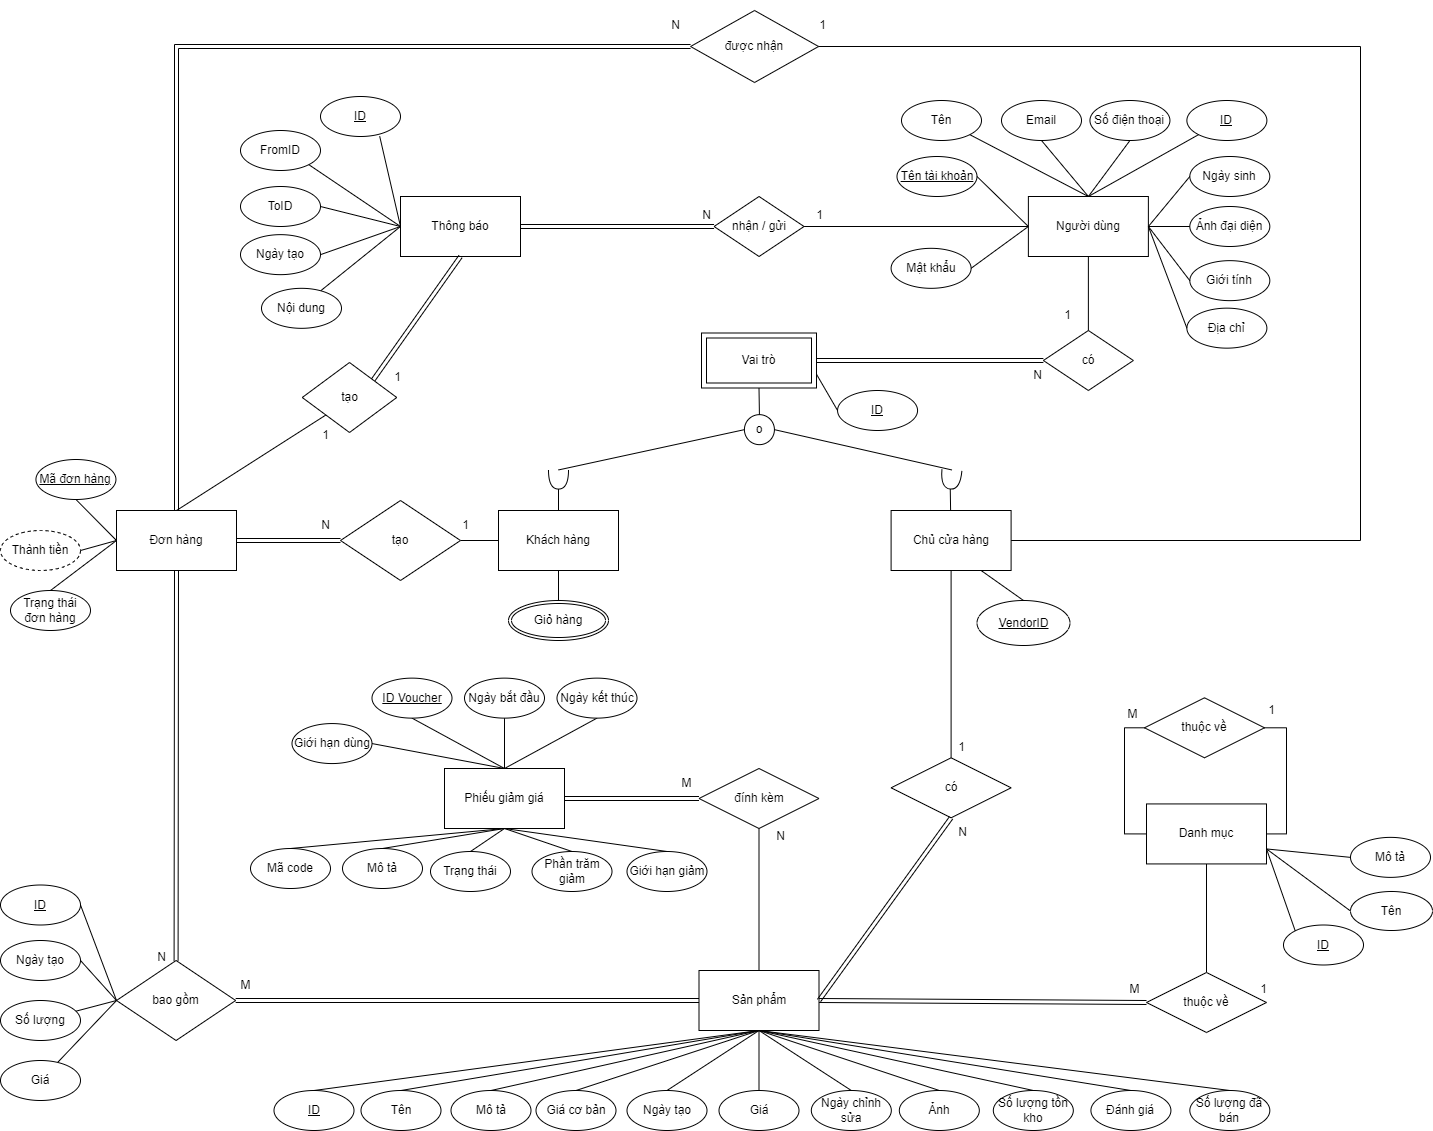
\includegraphics[width=1.1\linewidth]{Images/ERD.png}
        \vspace{1em}
        \caption{Lược đồ thực thể mối liên kết}
    \end{figure}
\subsection{Mô hình hoá cơ sở dữ liệu mức luận lý}
    \begin{figure}[H]
        \centering
        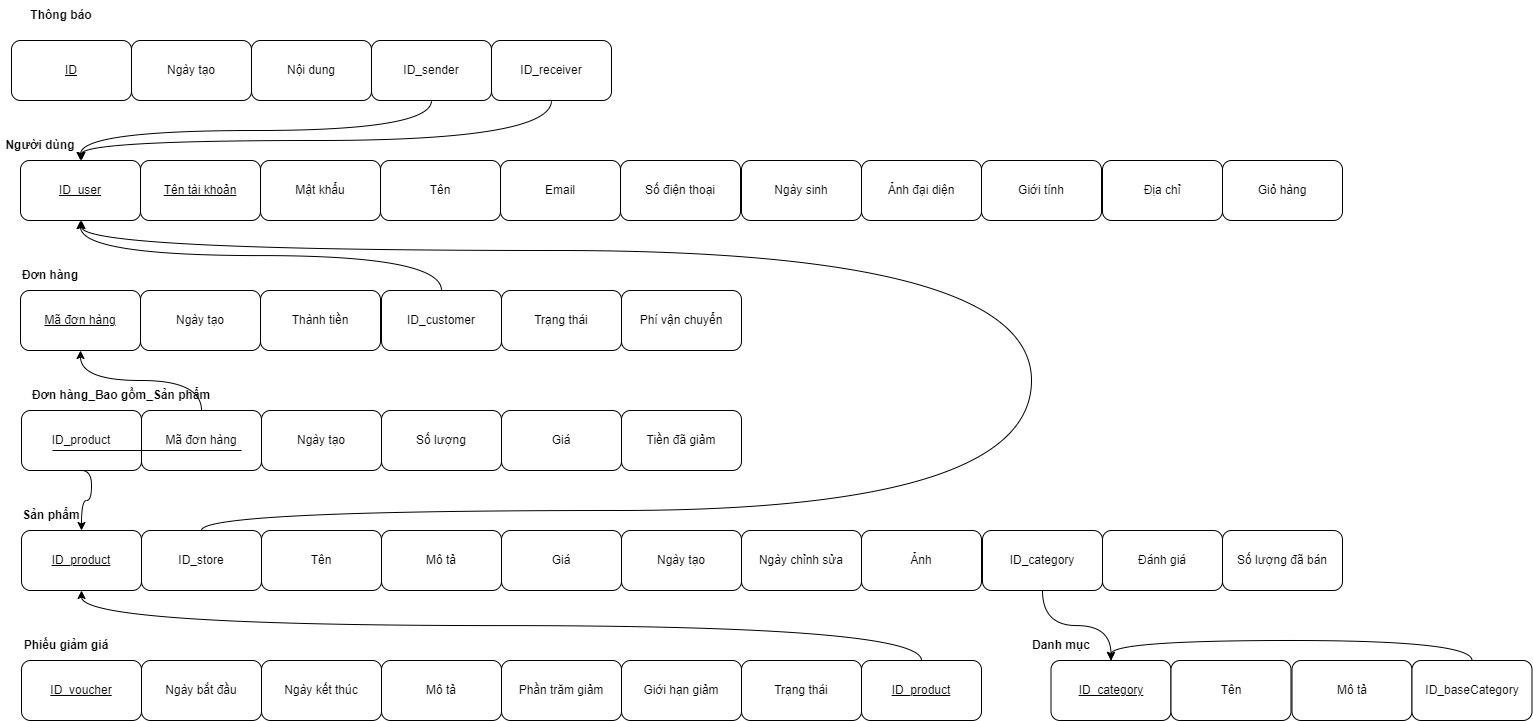
\includegraphics[width=1.1\linewidth]{Images/mapping.png}
        \vspace{1em}
        \caption{Mô hình dữ liệu quan hệ}
    \end{figure}
    \section{Kiến trúc hệ thống}
    \begin{figure}[h]
        \centering
        \includegraphics[width=0.6\linewidth]{Images/Roadside.png}
        \caption{Kiến trúc hệ thống}
    \end{figure}

% \section{Kiến trúc mạng}
% \begin{figure}[h]
%         \centering
%         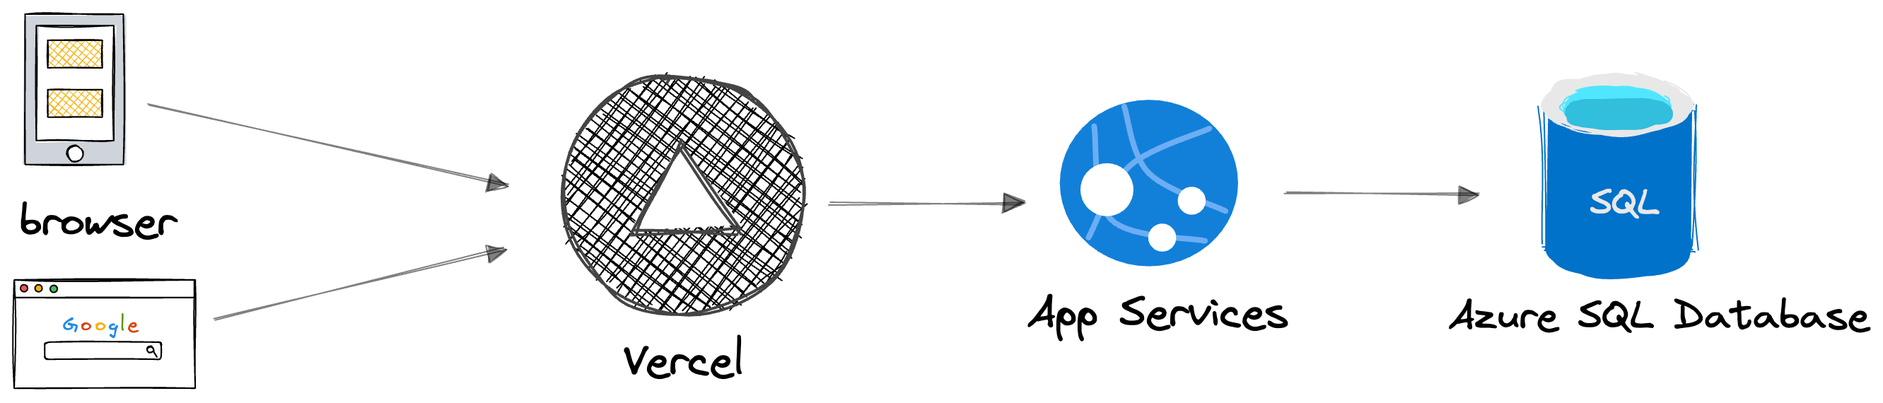
\includegraphics[width=0.8\linewidth]{Images/network.png}
%         \vspace{1em}
%         \caption{Kiến trúc mạng}
%         \label{fig:enter-label}
%     \end{figure}

% Kiến trúc này được triển khai để kết nối giữa người dùng cuối, nền tảng triển khai ứng dụng, và cơ sở dữ liệu. Các thành phần chính trong kiến trúc bao gồm:
% \begin{itemize}
%     \item \textbf{Browser (Trình duyệt):} Trình duyệt web và các thiết bị di động là điểm bắt đầu, nơi người dùng tương tác với ứng dụng web. Người dùng truy cập vào ứng dụng thông qua giao diện web, thực hiện các thao tác như đăng nhập, tìm kiếm, và quản lý thông tin.
%     \item \textbf{Vercel:} Vercel là nền tảng triển khai ứng dụng được sử dụng trong hệ thống này. Nó đảm bảo việc phân phối nội dung tĩnh và động một cách nhanh chóng và hiệu quả. Vercel chịu trách nhiệm triển khai và quản lý mã nguồn của ứng dụng web, đảm bảo rằng các yêu cầu từ phía người dùng được xử lý kịp thời và hiệu quả. Vercel nhận các yêu cầu từ trình duyệt, xử lý chúng và tương tác với các dịch vụ back-end để lấy dữ liệu cần thiết.
%     \item \textbf{App Services:} App Services đóng vai trò là server của hệ thống. Nó thực hiện các logic nghiệp vụ của ứng dụng, tương tác với cơ sở dữ liệu để xử lý và lưu trữ dữ liệu cần thiết. Các dịch vụ này chịu trách nhiệm xử lý các yêu cầu từ Vercel, thực hiện các tác vụ như xác thực người dùng, xử lý dữ liệu, và thực thi các quy trình nghiệp vụ của ứng dụng. App Services kết nối trực tiếp với cơ sở dữ liệu Azure SQL Database để truy xuất và cập nhật dữ liệu.
%     \item \textbf{Azure SQL Database:} Azure SQL Database là cơ sở dữ liệu chính của hệ thống. Nó chịu trách nhiệm lưu trữ và quản lý tất cả dữ liệu cần thiết cho ứng dụng. Cơ sở dữ liệu này đảm bảo tính toàn vẹn và bảo mật của dữ liệu, cung cấp khả năng truy xuất dữ liệu nhanh chóng và hiệu quả cho các dịch vụ ứng dụng. Dữ liệu từ App Services được lưu trữ và truy vấn trực tiếp từ Azure SQL Database, đảm bảo rằng mọi thông tin được lưu giữ an toàn và có thể truy cập nhanh chóng khi cần thiết.
    
% \end{itemize}

% Kiến trúc này đảm bảo rằng các thành phần trong hệ thống hoạt động cùng nhau một cách nhịp nhàng và hiệu quả. Trình duyệt và thiết bị di động của người dùng tương tác với Vercel, nền tảng triển khai ứng dụng, để gửi và nhận dữ liệu. Vercel đóng vai trò trung gian, chuyển tiếp các yêu cầu đến App Services, nơi thực hiện các logic nghiệp vụ và xử lý dữ liệu. App Services sau đó tương tác với Azure SQL Database để truy xuất và lưu trữ dữ liệu cần thiết, đảm bảo rằng hệ thống hoạt động mượt mà, hiệu quả và an toàn.\\

% Kiến trúc này không chỉ đảm bảo khả năng mở rộng và linh hoạt cho ứng dụng mà còn cung cấp một môi trường bảo mật và hiệu quả cho việc quản lý và xử lý dữ liệu. Sự kết hợp giữa các công nghệ hiện đại như Vercel, Azure App Services, và Azure SQL Database tạo ra một hệ thống mạnh mẽ, đáng tin cậy và dễ dàng bảo trì trong tương lai.

\section{API Endpoints}

\subsection{App Settings}

\subsubsection*{/api/settings - GET}
\begin{tabular}{|>{\raggedright\arraybackslash}p{3cm}|p{12cm}|}
\hline
\textbf{Operation} & GET \\
\hline
\textbf{Description} & Retrieve application settings. \\
\hline
\textbf{Responses} & 200: Success \\
\hline
\end{tabular}

\subsubsection*{/api/settings - POST}
\begin{tabular}{|>{\raggedright\arraybackslash}p{3cm}|p{12cm}|}
\hline
\textbf{Operation} & POST \\
\hline
\textbf{Description} & Create new application setting. \\
\hline
\textbf{Request Body} & AppSettings schema (JSON) \\
\hline
\textbf{Responses} & 200: Success \\
\hline
\end{tabular}

\subsubsection*{/api/settings - DELETE}
\begin{tabular}{|>{\raggedright\arraybackslash}p{3cm}|p{12cm}|}
\hline
\textbf{Operation} & DELETE \\
\hline
\textbf{Description} & Delete a specific setting based on ID. \\
\hline
\textbf{Parameters} & id: string (required) \\
\hline
\textbf{Responses} & 200: Success \\
\hline
\end{tabular}

\subsubsection*{/api/settings/update - POST}
\begin{tabular}{|>{\raggedright\arraybackslash}p{3cm}|p{12cm}|}
\hline
\textbf{Operation} & POST \\
\hline
\textbf{Description} & Update multiple settings in a single request. \\
\hline
\textbf{Request Body} & Array of AppSettings schema (JSON) \\
\hline
\textbf{Responses} & 200: Success \\
\hline
\end{tabular}

\subsection{Authentication}

\subsubsection*{/api/auth/signup - POST}
\begin{tabular}{|>{\raggedright\arraybackslash}p{3cm}|p{12cm}|}
\hline
\textbf{Operation} & POST \\
\hline
\textbf{Description} & Register a new account. \\
\hline
\textbf{Request Body} & Account schema (JSON) \\
\hline
\textbf{Responses} & 200: Success \\
\hline
\end{tabular}

\subsubsection*{/api/auth/login - POST}
\begin{tabular}{|>{\raggedright\arraybackslash}p{3cm}|p{12cm}|}
\hline
\textbf{Operation} & POST \\
\hline
\textbf{Description} & Authenticate a user and return a token. \\
\hline
\textbf{Request Body} & LoginInfo schema (JSON) \\
\hline
\textbf{Responses} & 200: Success \\
\hline
\end{tabular}

\subsubsection*{/api/auth/logout - POST}
\begin{tabular}{|>{\raggedright\arraybackslash}p{3cm}|p{12cm}|}
\hline
\textbf{Operation} & POST \\
\hline
\textbf{Description} & Log out a user and invalidate the session token. \\
\hline
\textbf{Responses} & 200: Success \\
\hline
\end{tabular}

\subsection{Orders}

\subsubsection*{/api/orders - GET}
\begin{tabular}{|>{\raggedright\arraybackslash}p{3cm}|p{12cm}|}
\hline
\textbf{Operation} & GET \\
\hline
\textbf{Description} & Retrieve all orders. \\
\hline
\textbf{Responses} & 200: Success \\
\hline
\end{tabular}

\subsubsection*{/api/orders - POST}
\begin{tabular}{|>{\raggedright\arraybackslash}p{3cm}|p{12cm}|}
\hline
\textbf{Operation} & POST \\
\hline
\textbf{Description} & Create a new order. \\
\hline
\textbf{Request Body} & Orders schema (JSON) \\
\hline
\textbf{Responses} & 200: Success \\
\hline
\end{tabular}

\subsubsection*{/api/orders - DELETE}
\begin{tabular}{|>{\raggedright\arraybackslash}p{3cm}|p{12cm}|}
\hline
\textbf{Operation} & DELETE \\
\hline
\textbf{Description} & Delete a specific order based on ID. \\
\hline
\textbf{Parameters} & id: string (required) \\
\hline
\textbf{Responses} & 200: Success \\
\hline
\end{tabular}

\subsubsection*{/api/orders/voucher - GET}
\begin{tabular}{|>{\raggedright\arraybackslash}p{3cm}|p{12cm}|}
\hline
\textbf{Operation} & GET \\
\hline
\textbf{Description} & Retrieve all vouchers associated with orders. \\
\hline
\textbf{Responses} & 200: Success \\
\hline
\end{tabular}

\subsubsection*{/api/orders/voucher - DELETE}
\begin{tabular}{|>{\raggedright\arraybackslash}p{3cm}|p{12cm}|}
\hline
\textbf{Operation} & DELETE \\
\hline
\textbf{Description} & Delete a voucher based on the given ID. \\
\hline
\textbf{Parameters} & id: string (required) \\
\hline
\textbf{Responses} & 200: Success \\
\hline
\end{tabular}

\subsubsection*{/api/orders/items - GET}
\begin{tabular}{|>{\raggedright\arraybackslash}p{3cm}|p{12cm}|}
\hline
\textbf{Operation} & GET \\
\hline
\textbf{Description} & Retrieve all items in all orders. \\
\hline
\textbf{Responses} & 200: Success \\
\hline
\end{tabular}

\subsubsection*{/api/orders/items - DELETE}
\begin{tabular}{|>{\raggedright\arraybackslash}p{3cm}|p{12cm}|}
\hline
\textbf{Operation} & DELETE \\
\hline
\textbf{Description} & Delete an item from an order based on the given ID. \\
\hline
\textbf{Parameters} & id: string (required) \\
\hline
\textbf{Responses} & 200: Success \\
\hline
\end{tabular}

\subsubsection*{/api/orders/update - POST}
\begin{tabular}{|>{\raggedright\arraybackslash}p{3cm}|p{12cm}|}
\hline
\textbf{Operation} & POST \\
\hline
\textbf{Description} & Update multiple orders in a single request. \\
\hline
\textbf{Request Body} & Array of Orders schema (JSON) \\
\hline
\textbf{Responses} & 200: Success \\
\hline
\end{tabular}

\subsection{Products}

\subsubsection*{/api/products - GET}
\begin{tabular}{|>{\raggedright\arraybackslash}p{3cm}|p{12cm}|}
\hline
\textbf{Operation} & GET \\
\hline
\textbf{Description} & Retrieve all products with details. \\
\hline
\textbf{Responses} & 200: Success, returns an array of products. \\
\hline
\end{tabular}

\subsubsection*{/api/products - POST}
\begin{tabular}{|>{\raggedright\arraybackslash}p{3cm}|p{12cm}|}
\hline
\textbf{Operation} & POST \\
\hline
\textbf{Description} & Create a new product entry with detailed specifications. \\
\hline
\textbf{Request Body} & Products schema (JSON) \\
\hline
\textbf{Responses} & 200: Success, product created. \\
\hline
\end{tabular}

\subsubsection*{/api/products - DELETE}
\begin{tabular}{|>{\raggedright\arraybackslash}p{3cm}|p{12cm}|}
\hline
\textbf{Operation} & DELETE \\
\hline
\textbf{Description} & Delete a specific product based on product ID. \\
\hline
\textbf{Parameters} & id: string (required) \\
\hline
\textbf{Responses} & 200: Success, product deleted. \\
\hline
\end{tabular}

\subsubsection*{/api/products/search - GET}
\begin{tabular}{|>{\raggedright\arraybackslash}p{3cm}|p{12cm}|}
\hline
\textbf{Operation} & GET \\
\hline
\textbf{Description} & Search for products by name. \\
\hline
\textbf{Parameters} & name: string (required) \\
\hline
\textbf{Responses} & 200: Success, returns matching products. \\
\hline
\end{tabular}

\subsubsection*{/api/products/{id} - GET}
\begin{tabular}{|>{\raggedright\arraybackslash}p{3cm}|p{12cm}|}
\hline
\textbf{Operation} & GET \\
\hline
\textbf{Description} & Retrieve detailed information about a product by ID. \\
\hline
\textbf{Parameters} & id: string (required) \\
\hline
\textbf{Responses} & 200: Success, returns product details. \\
\hline
\end{tabular}

\subsubsection*{/api/products/categories - GET}
\begin{tabular}{|>{\raggedright\arraybackslash}p{3cm}|p{12cm}|}
\hline
\textbf{Operation} & GET \\
\hline
\textbf{Description} & Retrieve all product categories. \\
\hline
\textbf{Responses} & 200: Success, returns categories array. \\
\hline
\end{tabular}

\subsubsection*{/api/products/categories - DELETE}
\begin{tabular}{|>{\raggedright\arraybackslash}p{3cm}|p{12cm}|}
\hline
\textbf{Operation} & DELETE \\
\hline
\textbf{Description} & Delete a specific category based on category ID. \\
\hline
\textbf{Parameters} & id: string (required) \\
\hline
\textbf{Responses} & 200: Success, category deleted. \\
\hline
\end{tabular}

\subsubsection*{/api/products/prices - GET}
\begin{tabular}{|>{\raggedright\arraybackslash}p{3cm}|p{12cm}|}
\hline
\textbf{Operation} & GET \\
\hline
\textbf{Description} & Retrieve pricing information for all products. \\
\hline
\textbf{Responses} & 200: Success, returns prices array. \\
\hline
\end{tabular}

\subsubsection*{/api/products/prices - DELETE}
\begin{tabular}{|>{\raggedright\arraybackslash}p{3cm}|p{12cm}|}
\hline
\textbf{Operation} & DELETE \\
\hline
\textbf{Description} & Delete pricing information based on price ID. \\
\hline
\textbf{Parameters} & id: string (required) \\
\hline
\textbf{Responses} & 200: Success, price information deleted. \\
\hline
\end{tabular}

\subsubsection*{/api/products/update - POST}
\begin{tabular}{|>{\raggedright\arraybackslash}p{3cm}|p{12cm}|}
\hline
\textbf{Operation} & POST \\
\hline
\textbf{Description} & Update multiple product entries in a single request. \\
\hline
\textbf{Request Body} & Array of Products schema (JSON) \\
\hline
\textbf{Responses} & 200: Success, products updated. \\
\hline
\end{tabular}

% \subsection{Stripe Integration}

% \subsubsection*{/api/stripe/customer/add - POST}
% \begin{tabular}{|>{\raggedright\arraybackslash}p{3cm}|p{12cm}|}
% \hline
% \textbf{Operation} & POST \\
% \hline
% \textbf{Description} & Adds a new customer to Stripe with credit card details. \\
% \hline
% \textbf{Request Body} & Includes Email, Name, and Credit Card details (Name, Number, Expiration, CVC). \\
% \hline
% \textbf{Responses} & 200: Success, returns the created Stripe customer object. \\
% \hline
% \end{tabular}

% \subsubsection*{/api/stripe/payment/add - POST}
% \begin{tabular}{|>{\raggedright\arraybackslash}p{3cm}|p{12cm}|}
% \hline
% \textbf{Operation} & POST \\
% \hline
% \textbf{Description} & Processes a payment via Stripe for a customer. \\
% \hline
% \textbf{Request Body} & AddStripePayment schema, includes customer ID, receipt email, and payment details. \\
% \hline
% \textbf{Responses} & 200: Success, returns the Stripe payment object. \\
% \hline
% \end{tabular}

% \subsubsection*{/api/stripe/create-checkout-session - POST}
% \begin{tabular}{|>{\raggedright\arraybackslash}p{3cm}|p{12cm}|}
% \hline
% \textbf{Operation} & POST \\
% \hline
% \textbf{Description} & Creates a Stripe checkout session for handling payments on the client side. \\
% \hline
% \textbf{Request Body} & CreateCheckoutSessionStripeRequest schema, includes product and pricing details. \\
% \hline
% \textbf{Responses} & 200: Success, returns session details for client-side handling. \\
% \hline
% \end{tabular}

\subsection{Users}

\subsubsection*{/api/users - GET}
\begin{tabular}{|>{\raggedright\arraybackslash}p{3cm}|p{12cm}|}
\hline
\textbf{Operation} & GET \\
\hline
\textbf{Description} & Retrieve a list of all users. \\
\hline
\textbf{Responses} & 200: Success, returns an array of user objects. \\
\hline
\end{tabular}

\subsubsection*{/api/users/update - POST}
\begin{tabular}{|>{\raggedright\arraybackslash}p{3cm}|p{12cm}|}
\hline
\textbf{Operation} & POST \\
\hline
\textbf{Description} & Update multiple user profiles in a single request. \\
\hline
\textbf{Request Body} & Array of Users schema (JSON), allowing batch updates. \\
\hline
\textbf{Responses} & 200: Success, users updated. \\
\hline
\end{tabular}

\subsubsection*{/api/users/account - GET}
\begin{tabular}{|>{\raggedright\arraybackslash}p{3cm}|p{12cm}|}
\hline
\textbf{Operation} & GET \\
\hline
\textbf{Description} & Retrieve account details for the logged-in user. \\
\hline
\textbf{Responses} & 200: Success, returns user account details. \\
\hline
\end{tabular}

\subsubsection*{/api/users/account - DELETE}
\begin{tabular}{|>{\raggedright\arraybackslash}p{3cm}|p{12cm}|}
\hline
\textbf{Operation} & DELETE \\
\hline
\textbf{Description} & Delete a user account based on the given ID. \\
\hline
\textbf{Parameters} & id: string, UUID (required) \\
\hline
\textbf{Responses} & 200: Success, account deleted. \\
\hline
\end{tabular}

% Add more tables for other endpoints as needed


    
    
\section{Hiện thực}
\label{chap:Implementation}
$\indent$Giao diện hệ thống sử dụng màu chủ đạo là xanh lá với trên nền trắng. Màu trắng đại diện cho sự tinh khiết, sạch sẽ và thanh lịch, trong khi màu xanh lá tượng trưng cho sự tươi mới và sự sống. Màu xanh lá có thể tạo được cảm giác tươi mát và gắn kết với sản phẩm nông nghiệp. Sự kết hợp giữa màu xanh lá và trắng tạo ra một cảm giác tự nhiên, tươi mới và gợi nhớ về một môi trường xanh mát. Nó cũng tạo ra một sự tương phản mạnh mẽ, thu hút sự chú ý của khách truy cập và tạo nên một trải nghiệm trực quan dễ nhìn.

\subsection{Header - Footer}
$\indent$Trên đầu mỗi trang đều có một thanh header để điều hướng sang các trang khác như trang chủ, giỏ hàng, thông tin người dùng,...
    \begin{figure}[H]
        \begin{center}
        
\includegraphics[width=1\linewidth]{Images/UI/header.png}
        \end{center}
        \caption{Header}
    \end{figure}

Cuối mỗi trang sẽ có footer hiển thị một số thông tin về sàn cũng như một số link chuyển hướng nhanh sang các nghiệp vụ khác mà san cung cấp.
\begin{figure}[h]
    \centering
    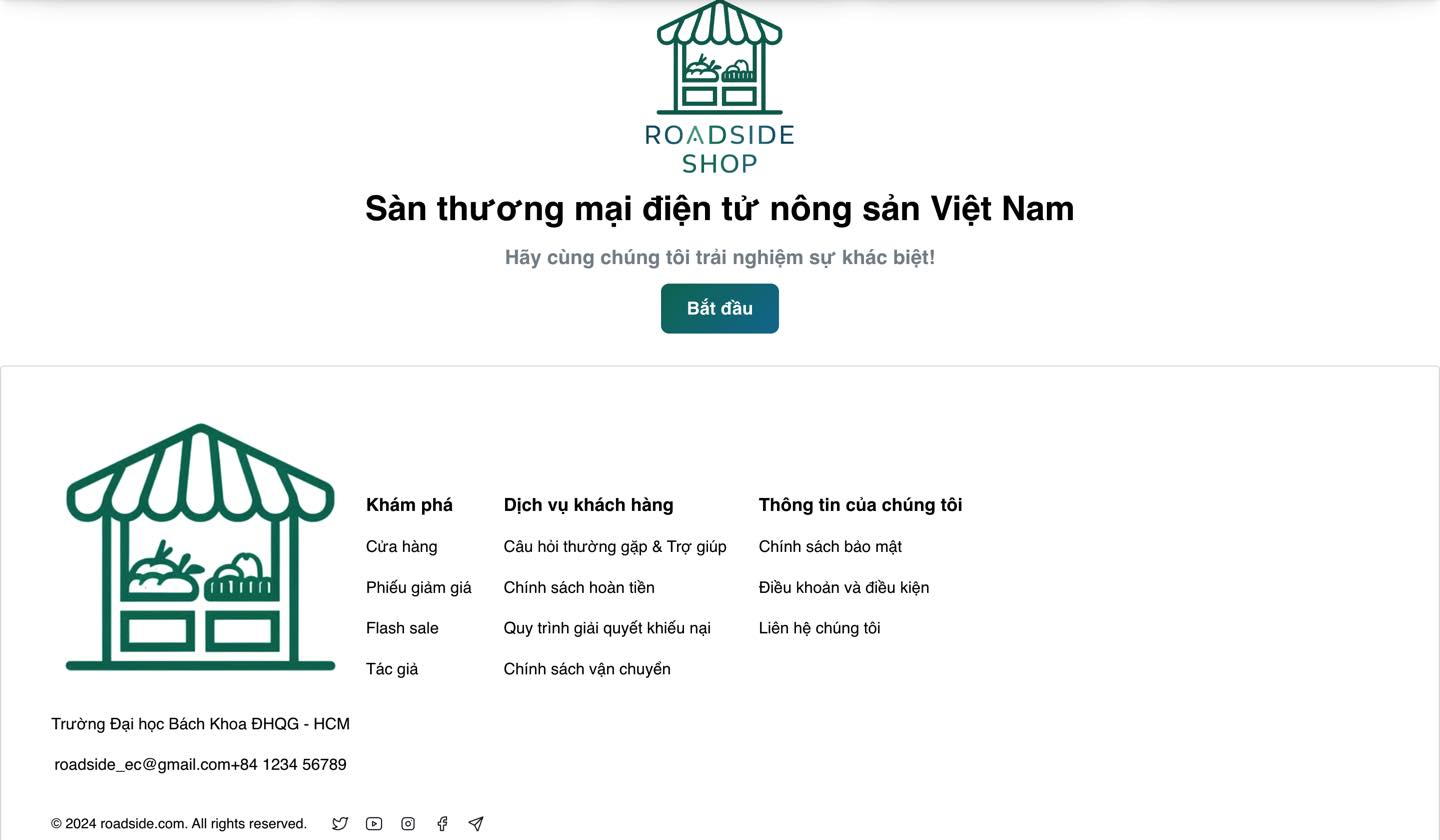
\includegraphics[width=1\linewidth]{Images/UI/footer.png}
    \vspace{1em}
    \caption{Footer}
\end{figure}
\subsection{Đăng nhập - Đăng ký}
$\indent$Trang đăng nhập được thiết kế để người dùng có thể đăng nhập vào tài khoản của họ. Giao diện bao gồm một form đăng nhập với hai trường nhập liệu cho tên người dùng và mật khẩu, cùng với nút "Đăng nhập". Trang cũng cung cấp liên kết "Quên mật khẩu" để người dùng khôi phục mật khẩu nếu cần, và liên kết "Đăng ký" để chuyển hướng người dùng đến trang đăng ký.
    \begin{figure}[H]
        \begin{center}
        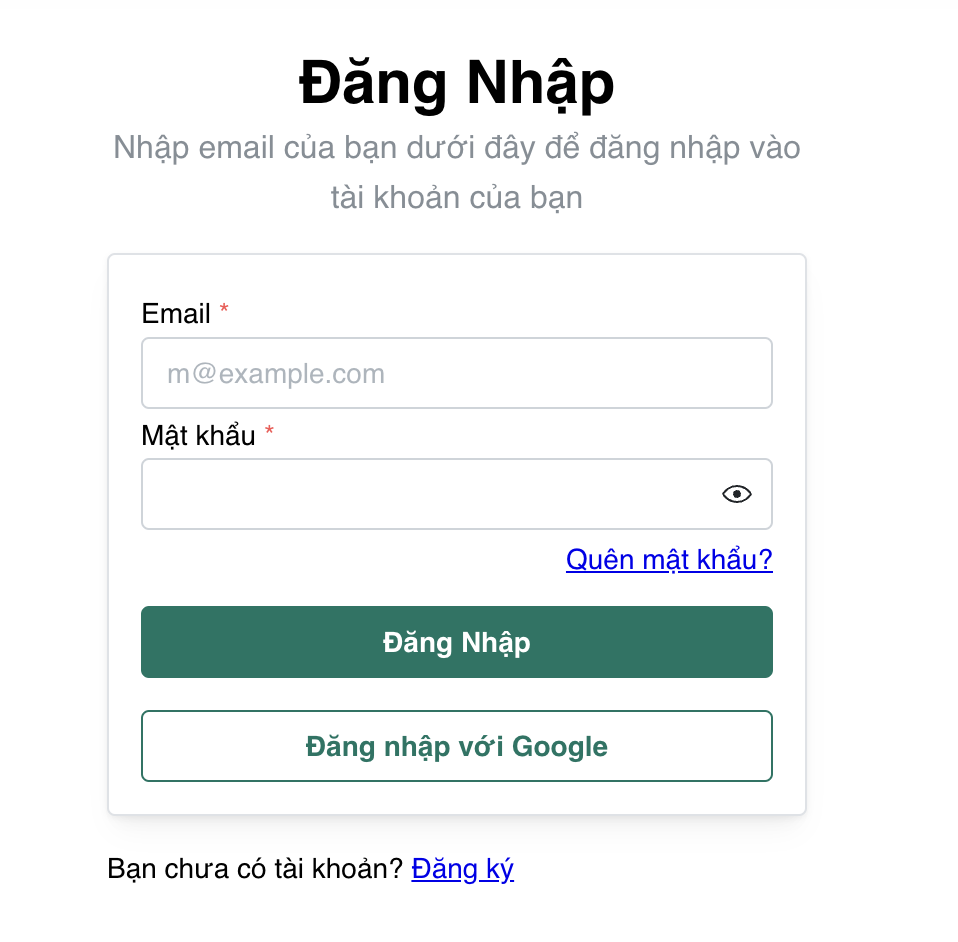
\includegraphics[width=0.6\linewidth]{Images/UI/signin.png}
        \end{center}
        \caption{Trang đăng nhập}
    \end{figure}
Trang đăng ký cho phép người dùng tạo một tài khoản mới trên hệ thống. Trang có cấu trúc tương tự với trang đăng nhập, bao gồm form đăng ký với các trường nhập liệu cho tên người dùng, địa chỉ email, mật khẩu và xác nhận mật khẩu, cùng với nút "Đăng ký". Ngoài ra, trang cũng cung cấp liên kết "Đăng nhập" để người dùng có thể chuyển hướng đến trang đăng nhập.
\begin{figure}[h]
    \centering
    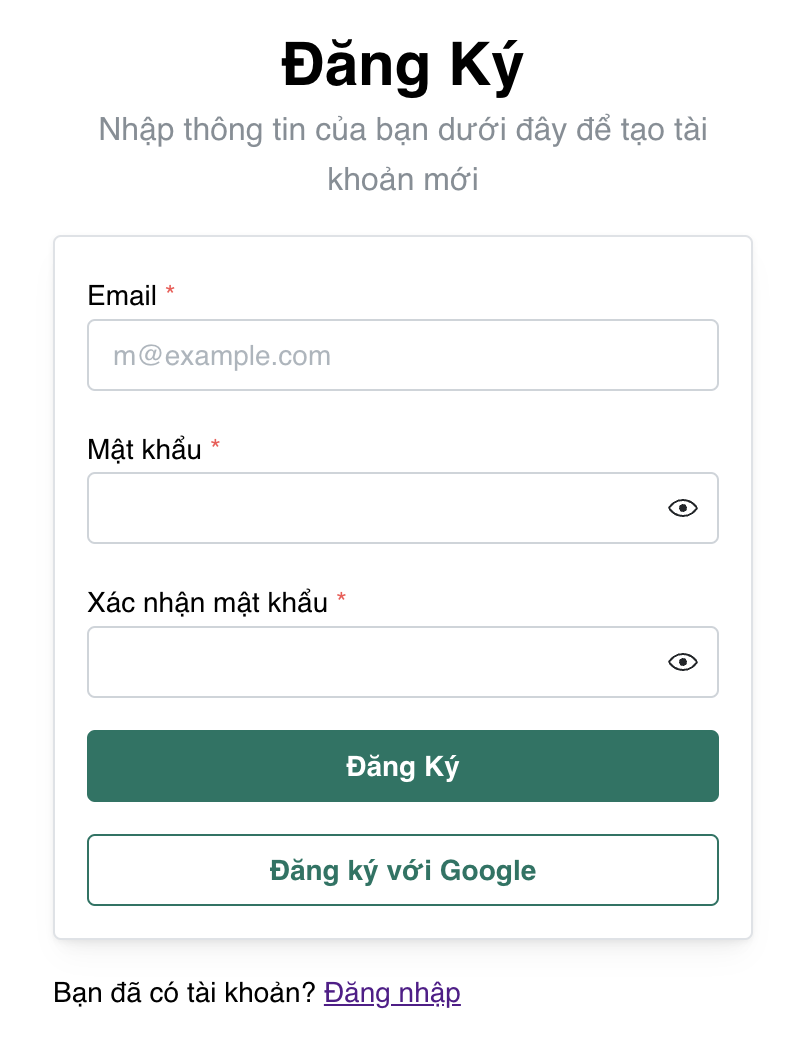
\includegraphics[width=0.5\linewidth]{Images/UI/signup.png}
    \vspace{1em}
    \caption{Trang đăng ký}
\end{figure}

\newpage
\subsection{Trang chủ}
$\indent$Trang chủ hiển thị thông tin tổng quan về các loại danh mục sản phẩm và danh sách các sản phẩm nông sản.     
\begin{figure}[H]
    \centering
    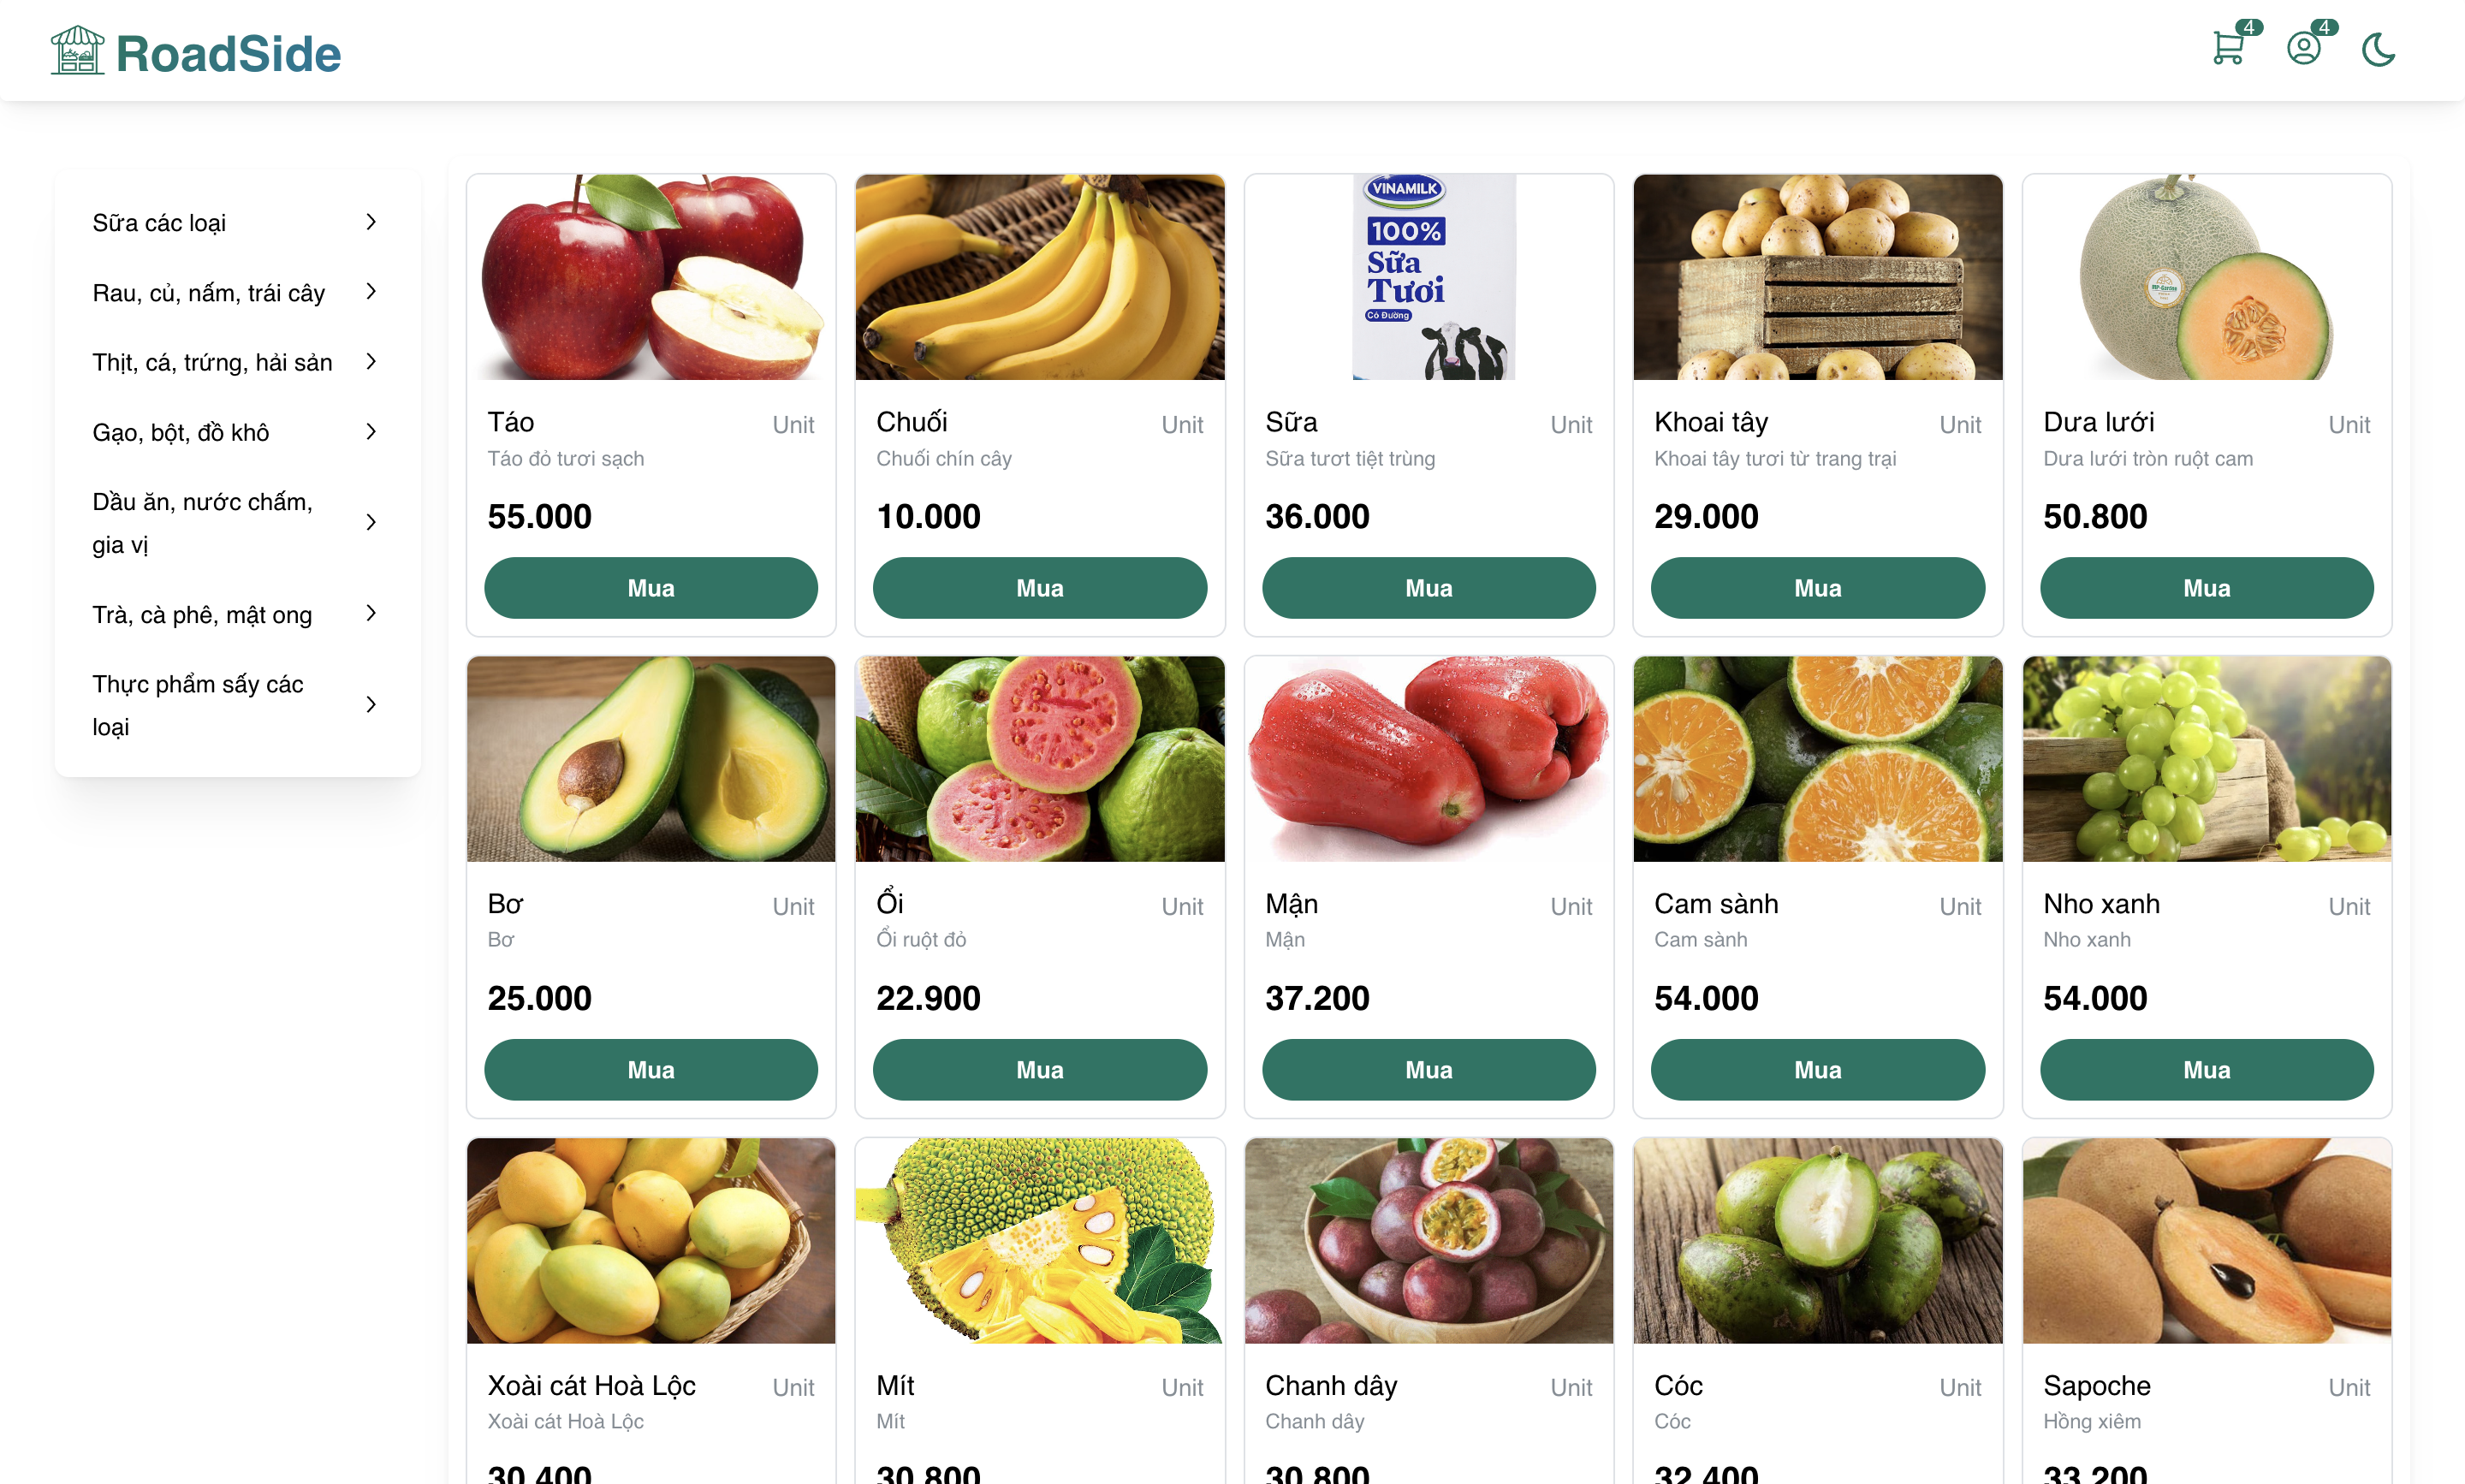
\includegraphics[scale=0.3] {Images/UI/Homepage.png}
    \vspace{2em}
    \caption{Trang chủ}
\end{figure}


Phía bên trái là danh mục các loại sản phẩm được phân loại theo từng đặc trưng riêng.
\begin{figure}[H]
    \centering
    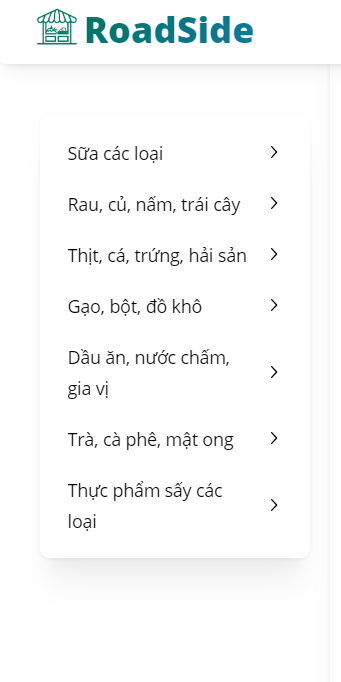
\includegraphics[scale=0.7] {Images/UI/category1.png}
    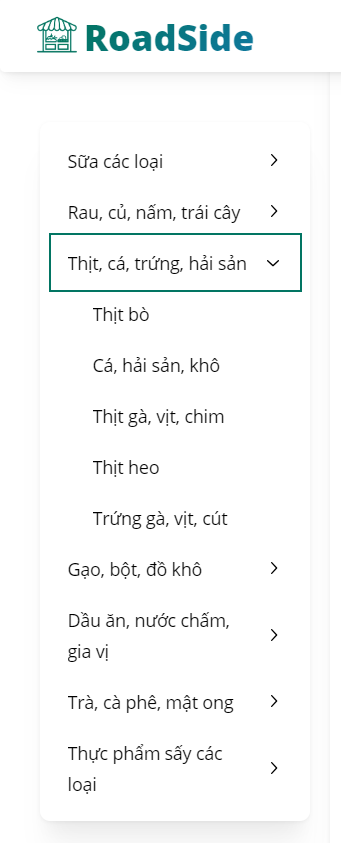
\includegraphics[scale=0.7] {Images/UI/category2.png}
    \vspace{1em}
    \caption{Danh mục sản phẩm}
\end{figure}

Sau khi chọn loại sản phẩm cần mua, danh sách các sản phẩm đã được phân loại sẽ hiện ra ở bên phải.
\begin{figure}[H]
    \centering
    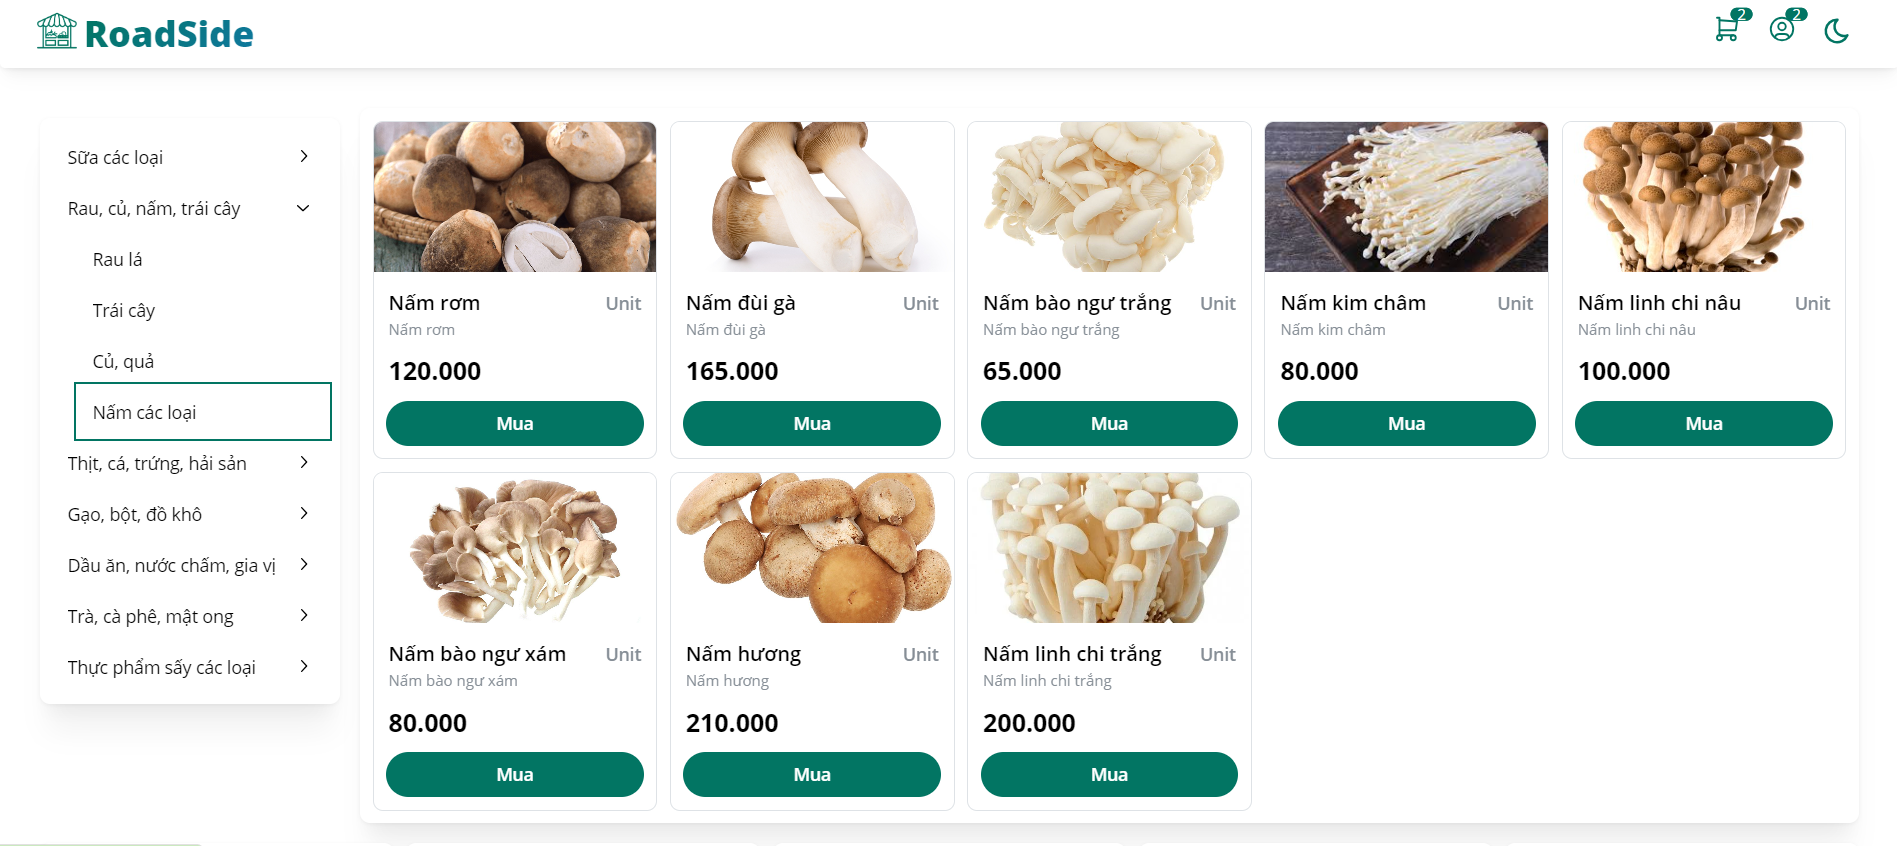
\includegraphics[width=1\linewidth] {Images/UI/product_category.png}
\end{figure}
\begin{figure}[H]
    \centering
    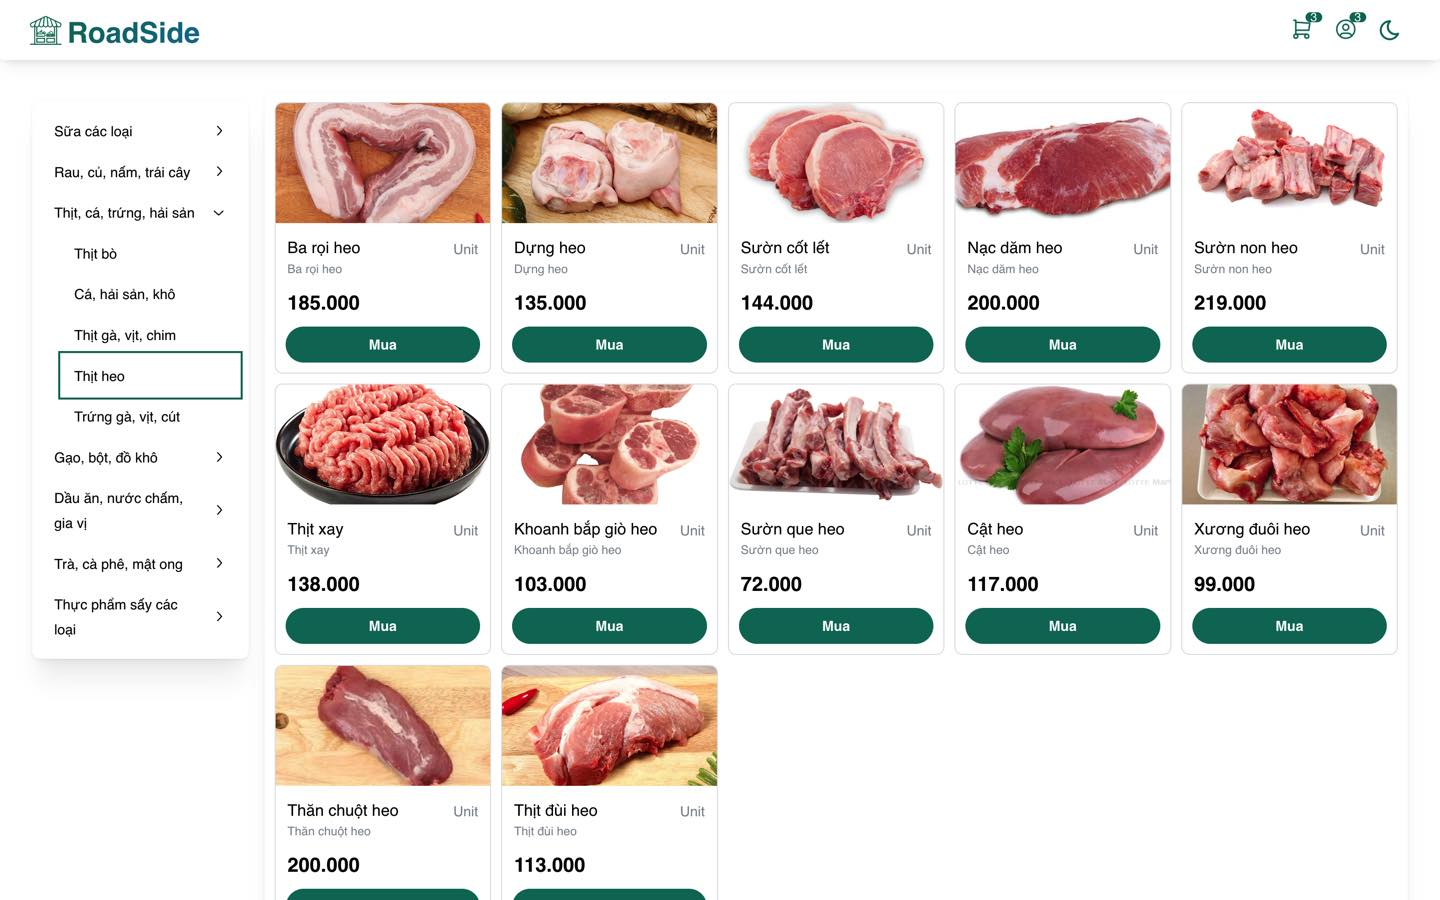
\includegraphics[width=1\linewidth] {Images/UI/categories2.png}
\end{figure}
\begin{figure}[H]
    \centering
    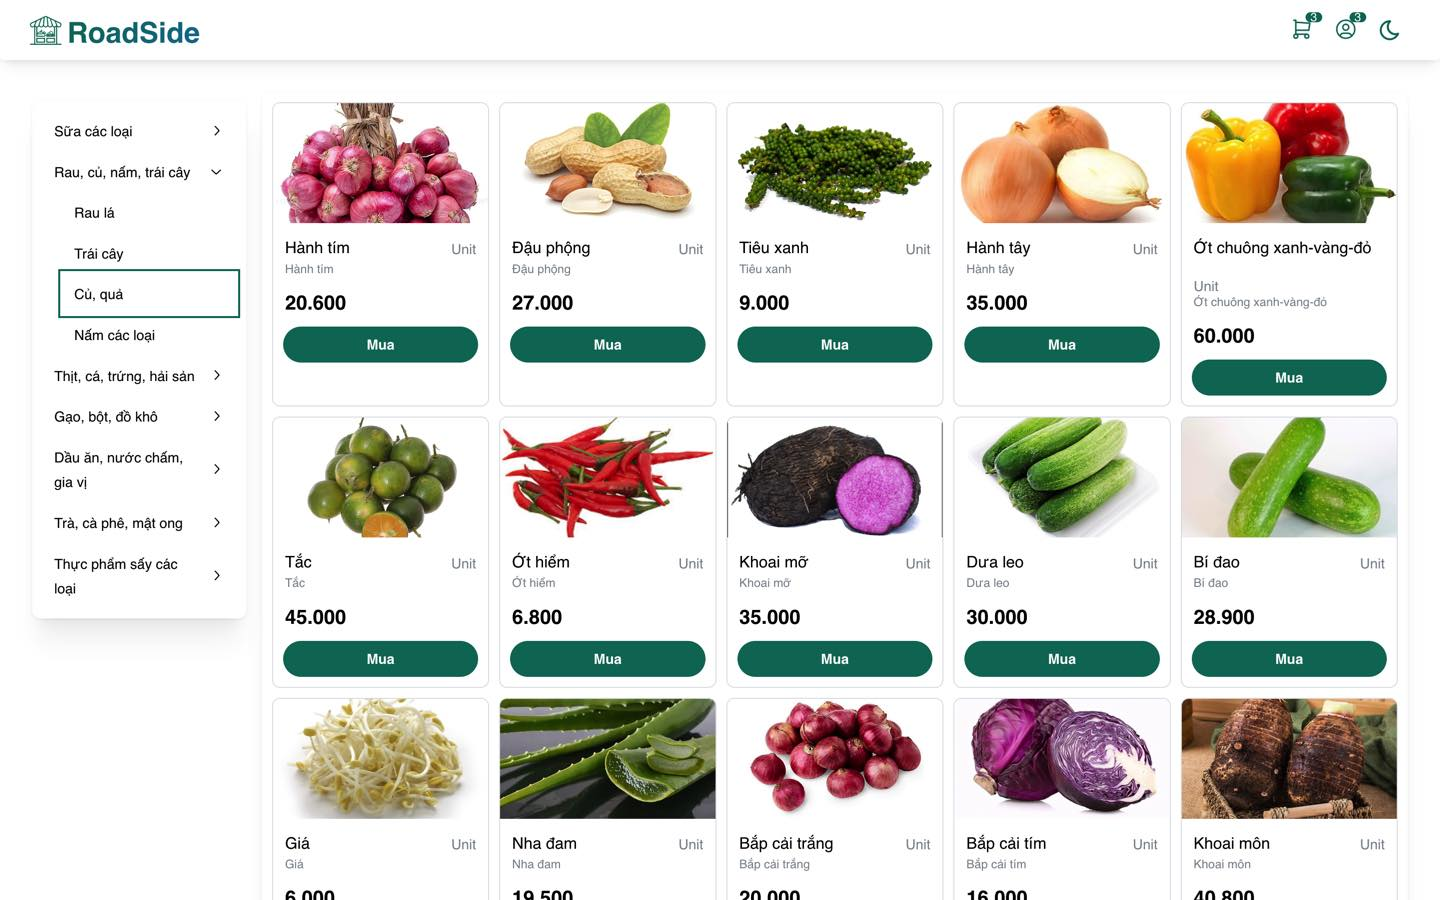
\includegraphics[width=1\linewidth] {Images/UI/categories3.png}
\end{figure}
\begin{figure}[H]
    \centering
    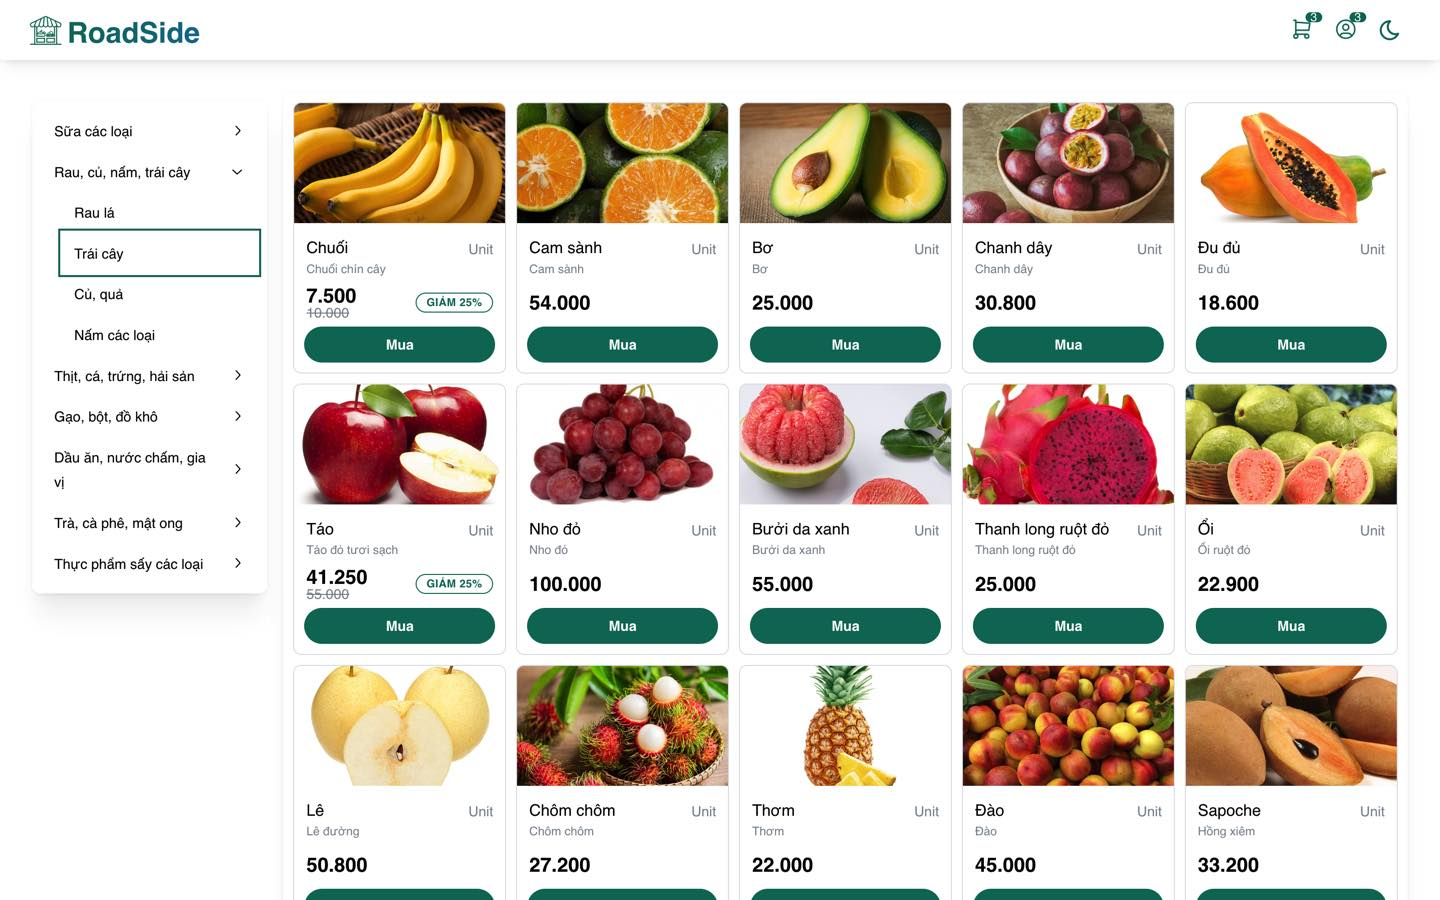
\includegraphics[width=1\linewidth] {Images/UI/categories4.png}
\end{figure}
\begin{figure}[H]
    \centering
    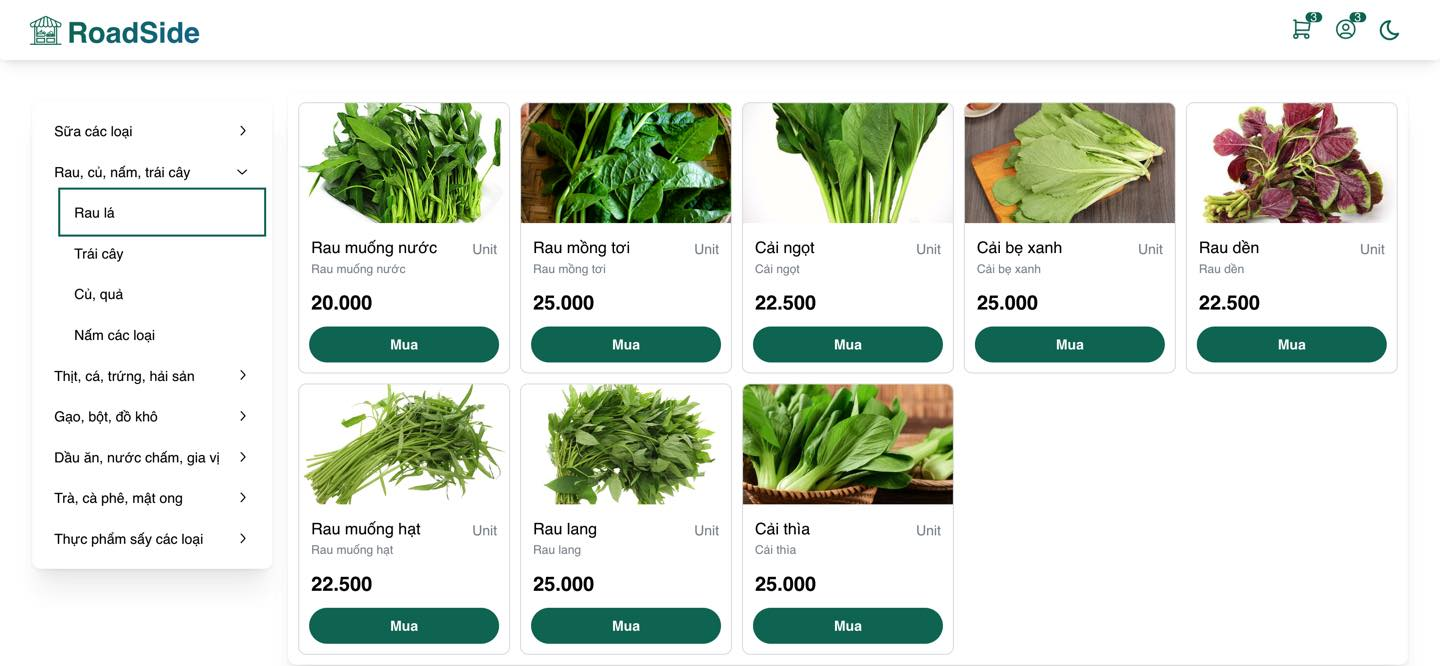
\includegraphics[width=1\linewidth] {Images/UI/categories6.png}
    \vspace{1em}
    \caption{Phân loại sản phẩm theo danh mục}
\end{figure}
\subsection{Thông tin sản phẩm}
$\indent$Ở trang chủ mỗi sản phẩm sẽ được hiển thị dưới dạng một thẻ sản phẩm, bao gồm các thông tin cơ bản như tên, giá, hình ảnh mô tả và giá giảm (nếu có).
\begin{figure}[H]
    \centering
    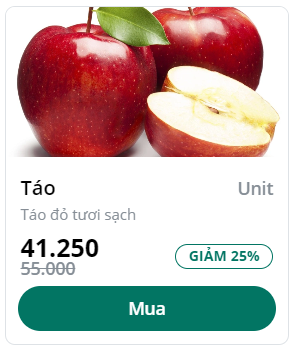
\includegraphics[scale=1] {Images/UI/product_card.png}
    \vspace{1em}
    \caption{Thẻ sản phẩm}
\end{figure}

Nếu bấm vào thẻ sản phẩm, sẽ được chuyển hướng đến trang xem thông tin chi tiết của sản phẩm đó.
\begin{figure}[H]
    \centering
    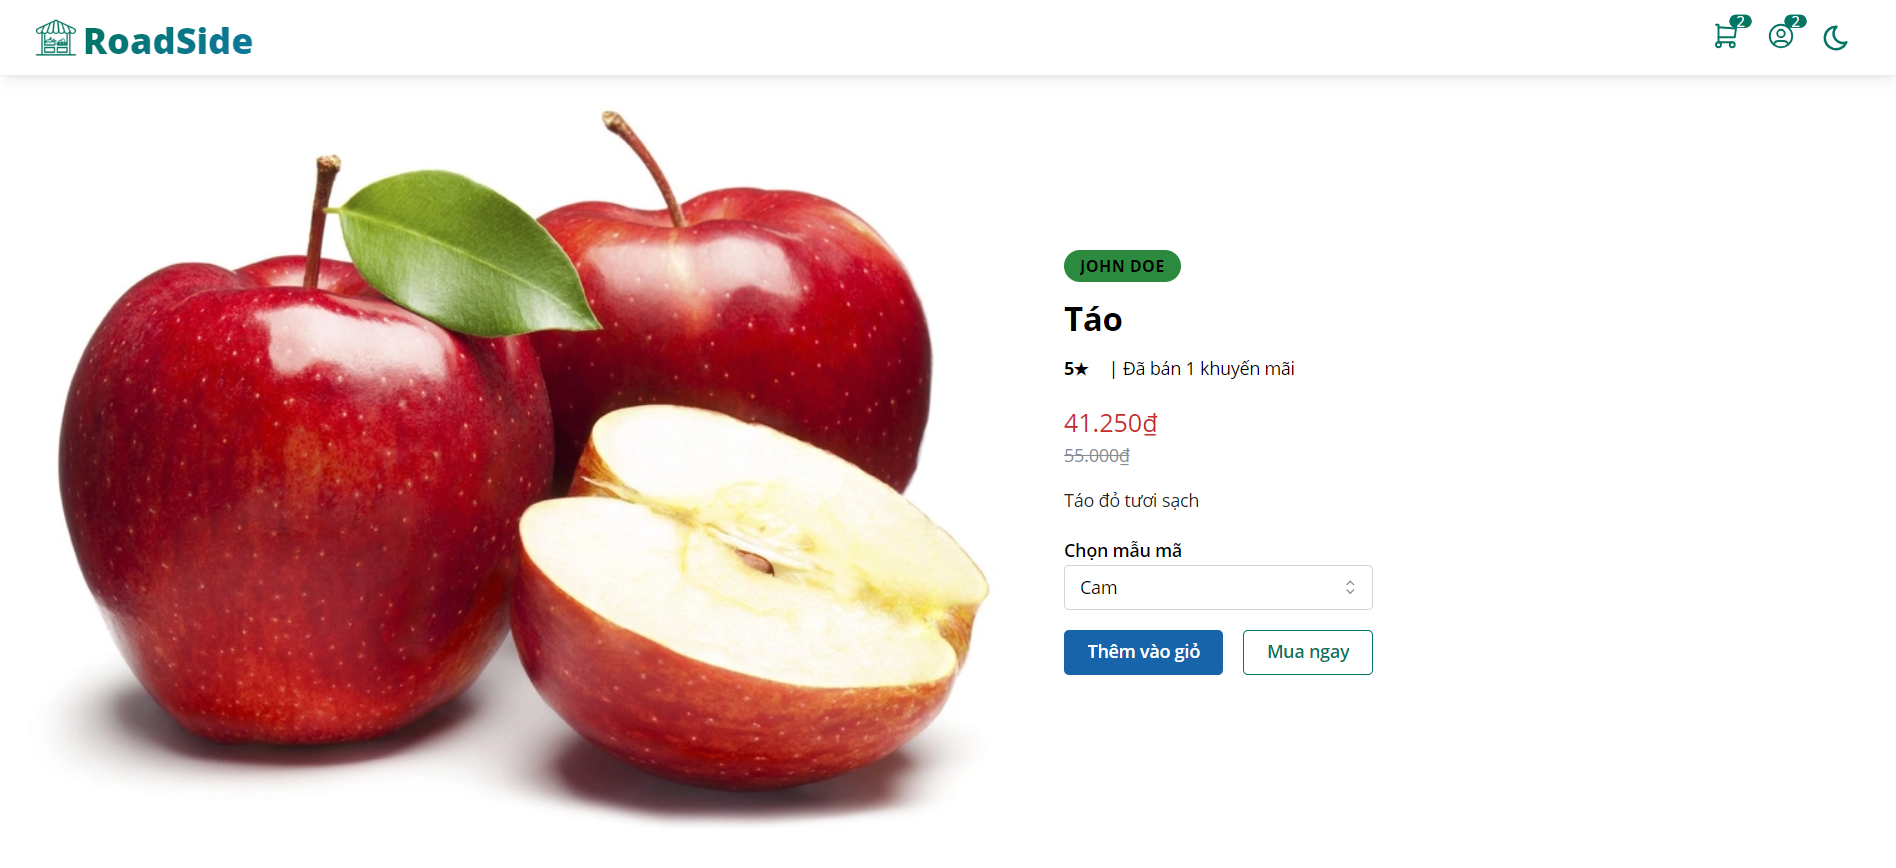
\includegraphics[width=1\linewidth] {Images/UI/product_details.png}
    \vspace{1em}
    \caption{Trang thông tin sản phẩm chi tiết}
\end{figure}

\subsection{Đặt hàng}
Sau khi đăng nhập vào hệ thống, nếu nhấn vào biểu tượng giỏ hàng trên thanh navbar, trang giỏ hàng sẽ hiện ra. Khách hàng có thể xem thông tin về các sản phẩm mà người dùng đã thêm vào giỏ hàng, bao gồm thông tin về tên, hình ảnh, giá và số lượng. Ở đây người dùng có thể xem lại và điều chỉnh các mục trong giỏ hàng trước khi đặt hàng. Người dùng có thể thay đổi số lượng hoặc xóa sản phẩm khỏi giỏ hàng.
    \begin{figure}[H]
        \centering
        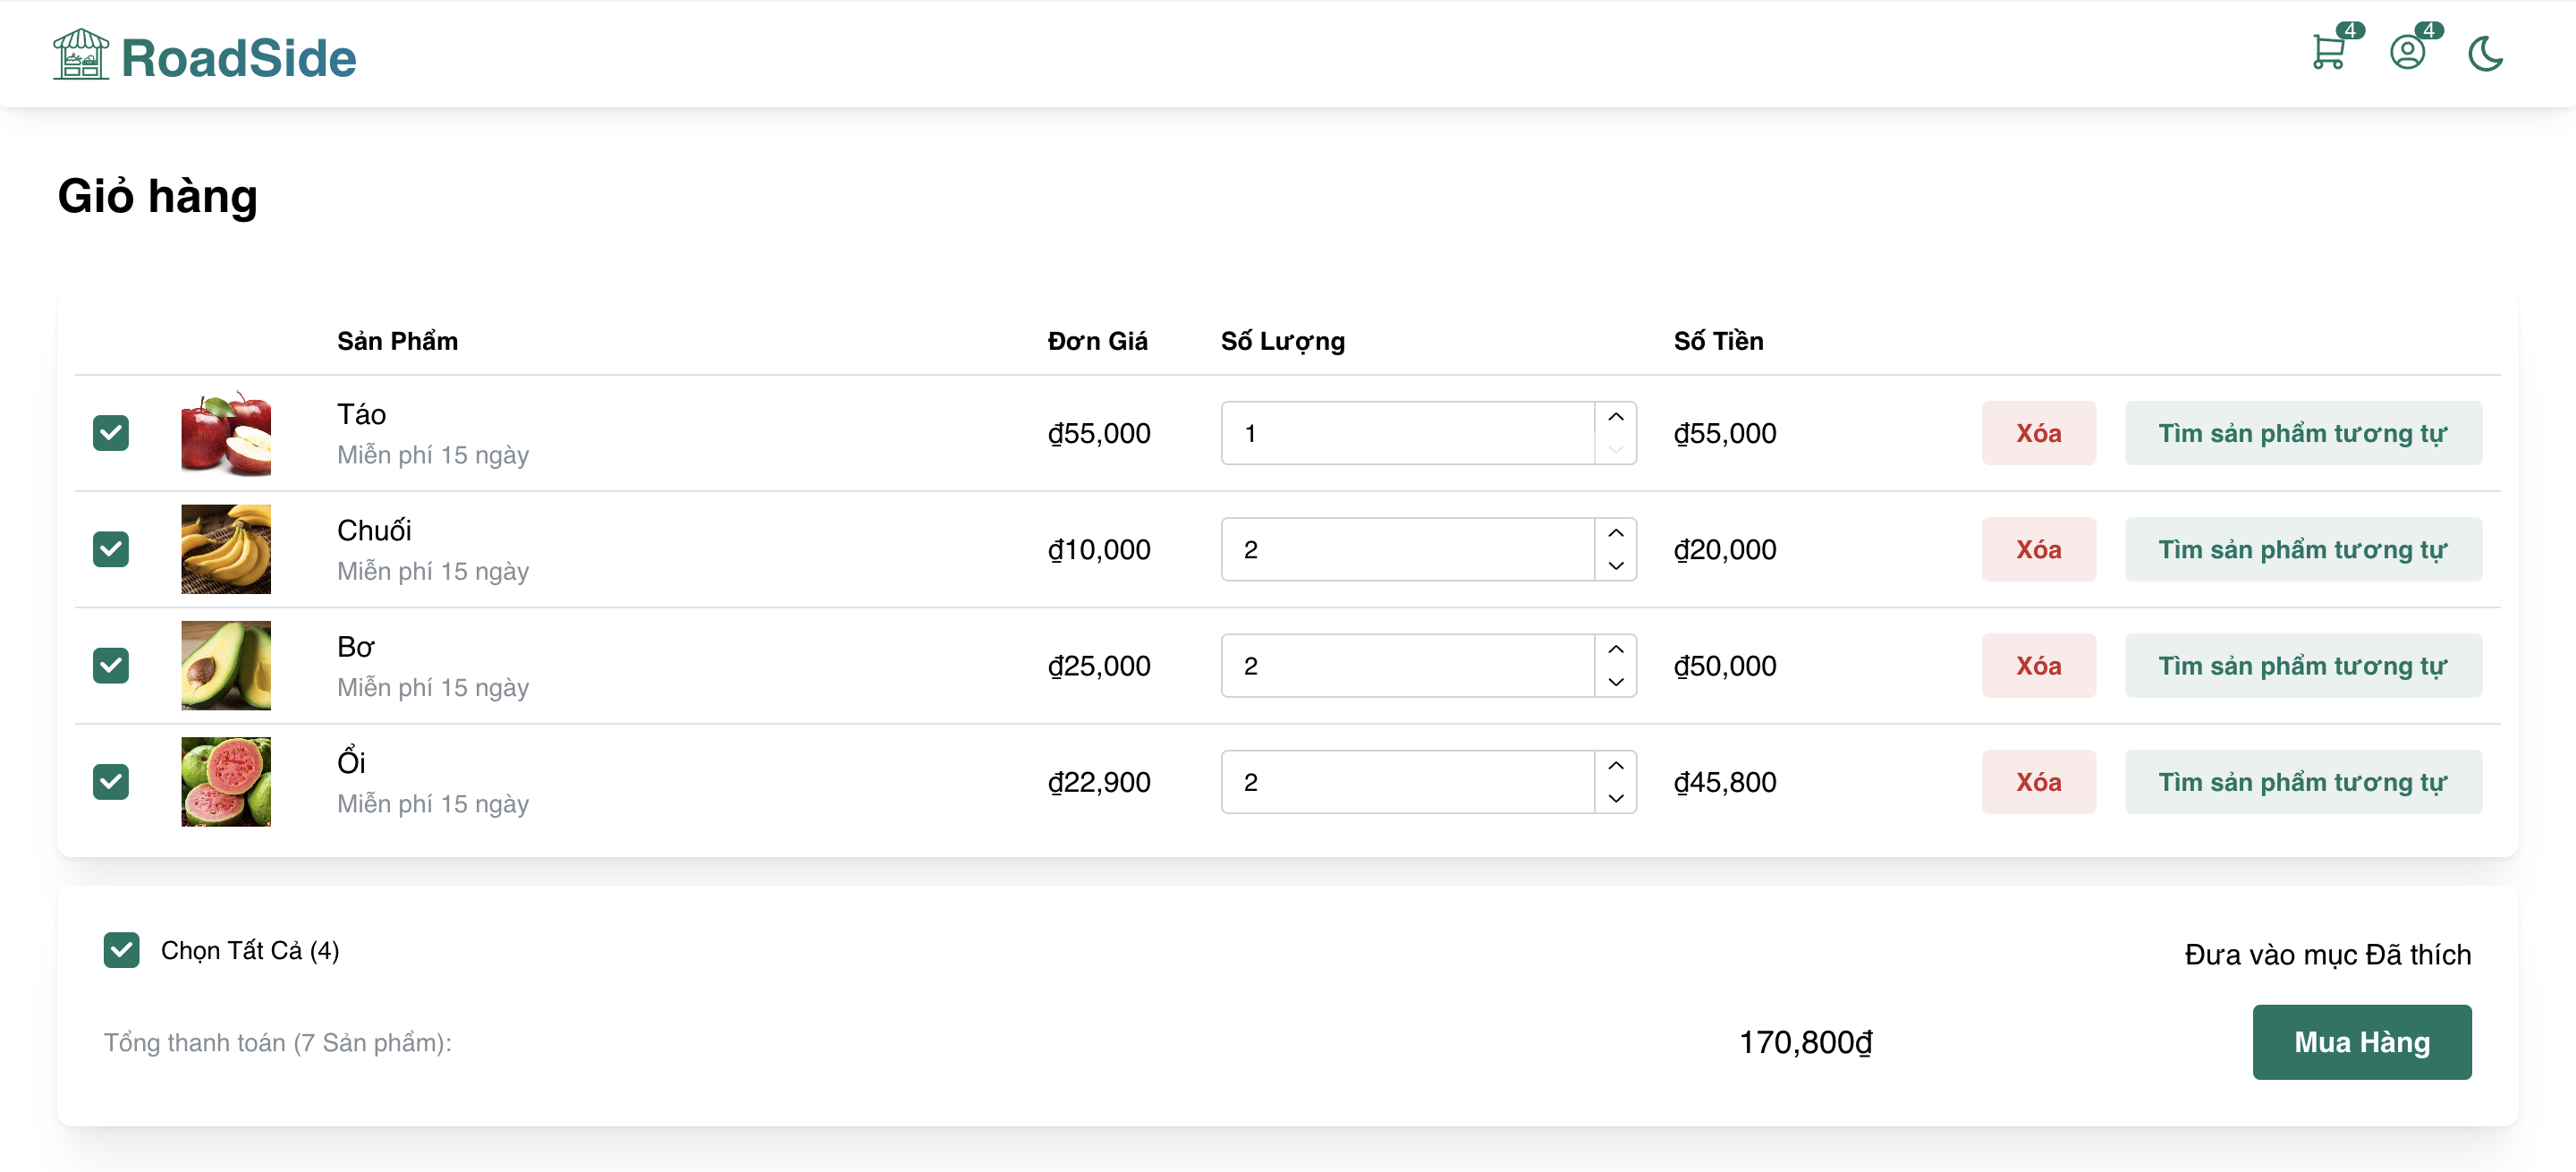
\includegraphics[width=1\linewidth] {Images/UI/cart.png}
        \vspace{1em}
        \caption{Giỏ hàng}
    \end{figure}

Bấm nút "Đặt hàng" để tiến hành tạo đơn hàng, một modal được hiện lên để xác nhận lại thông tin đặt hàng và phương thức thanh toán.

    \begin{figure}[H]
        \begin{center}
        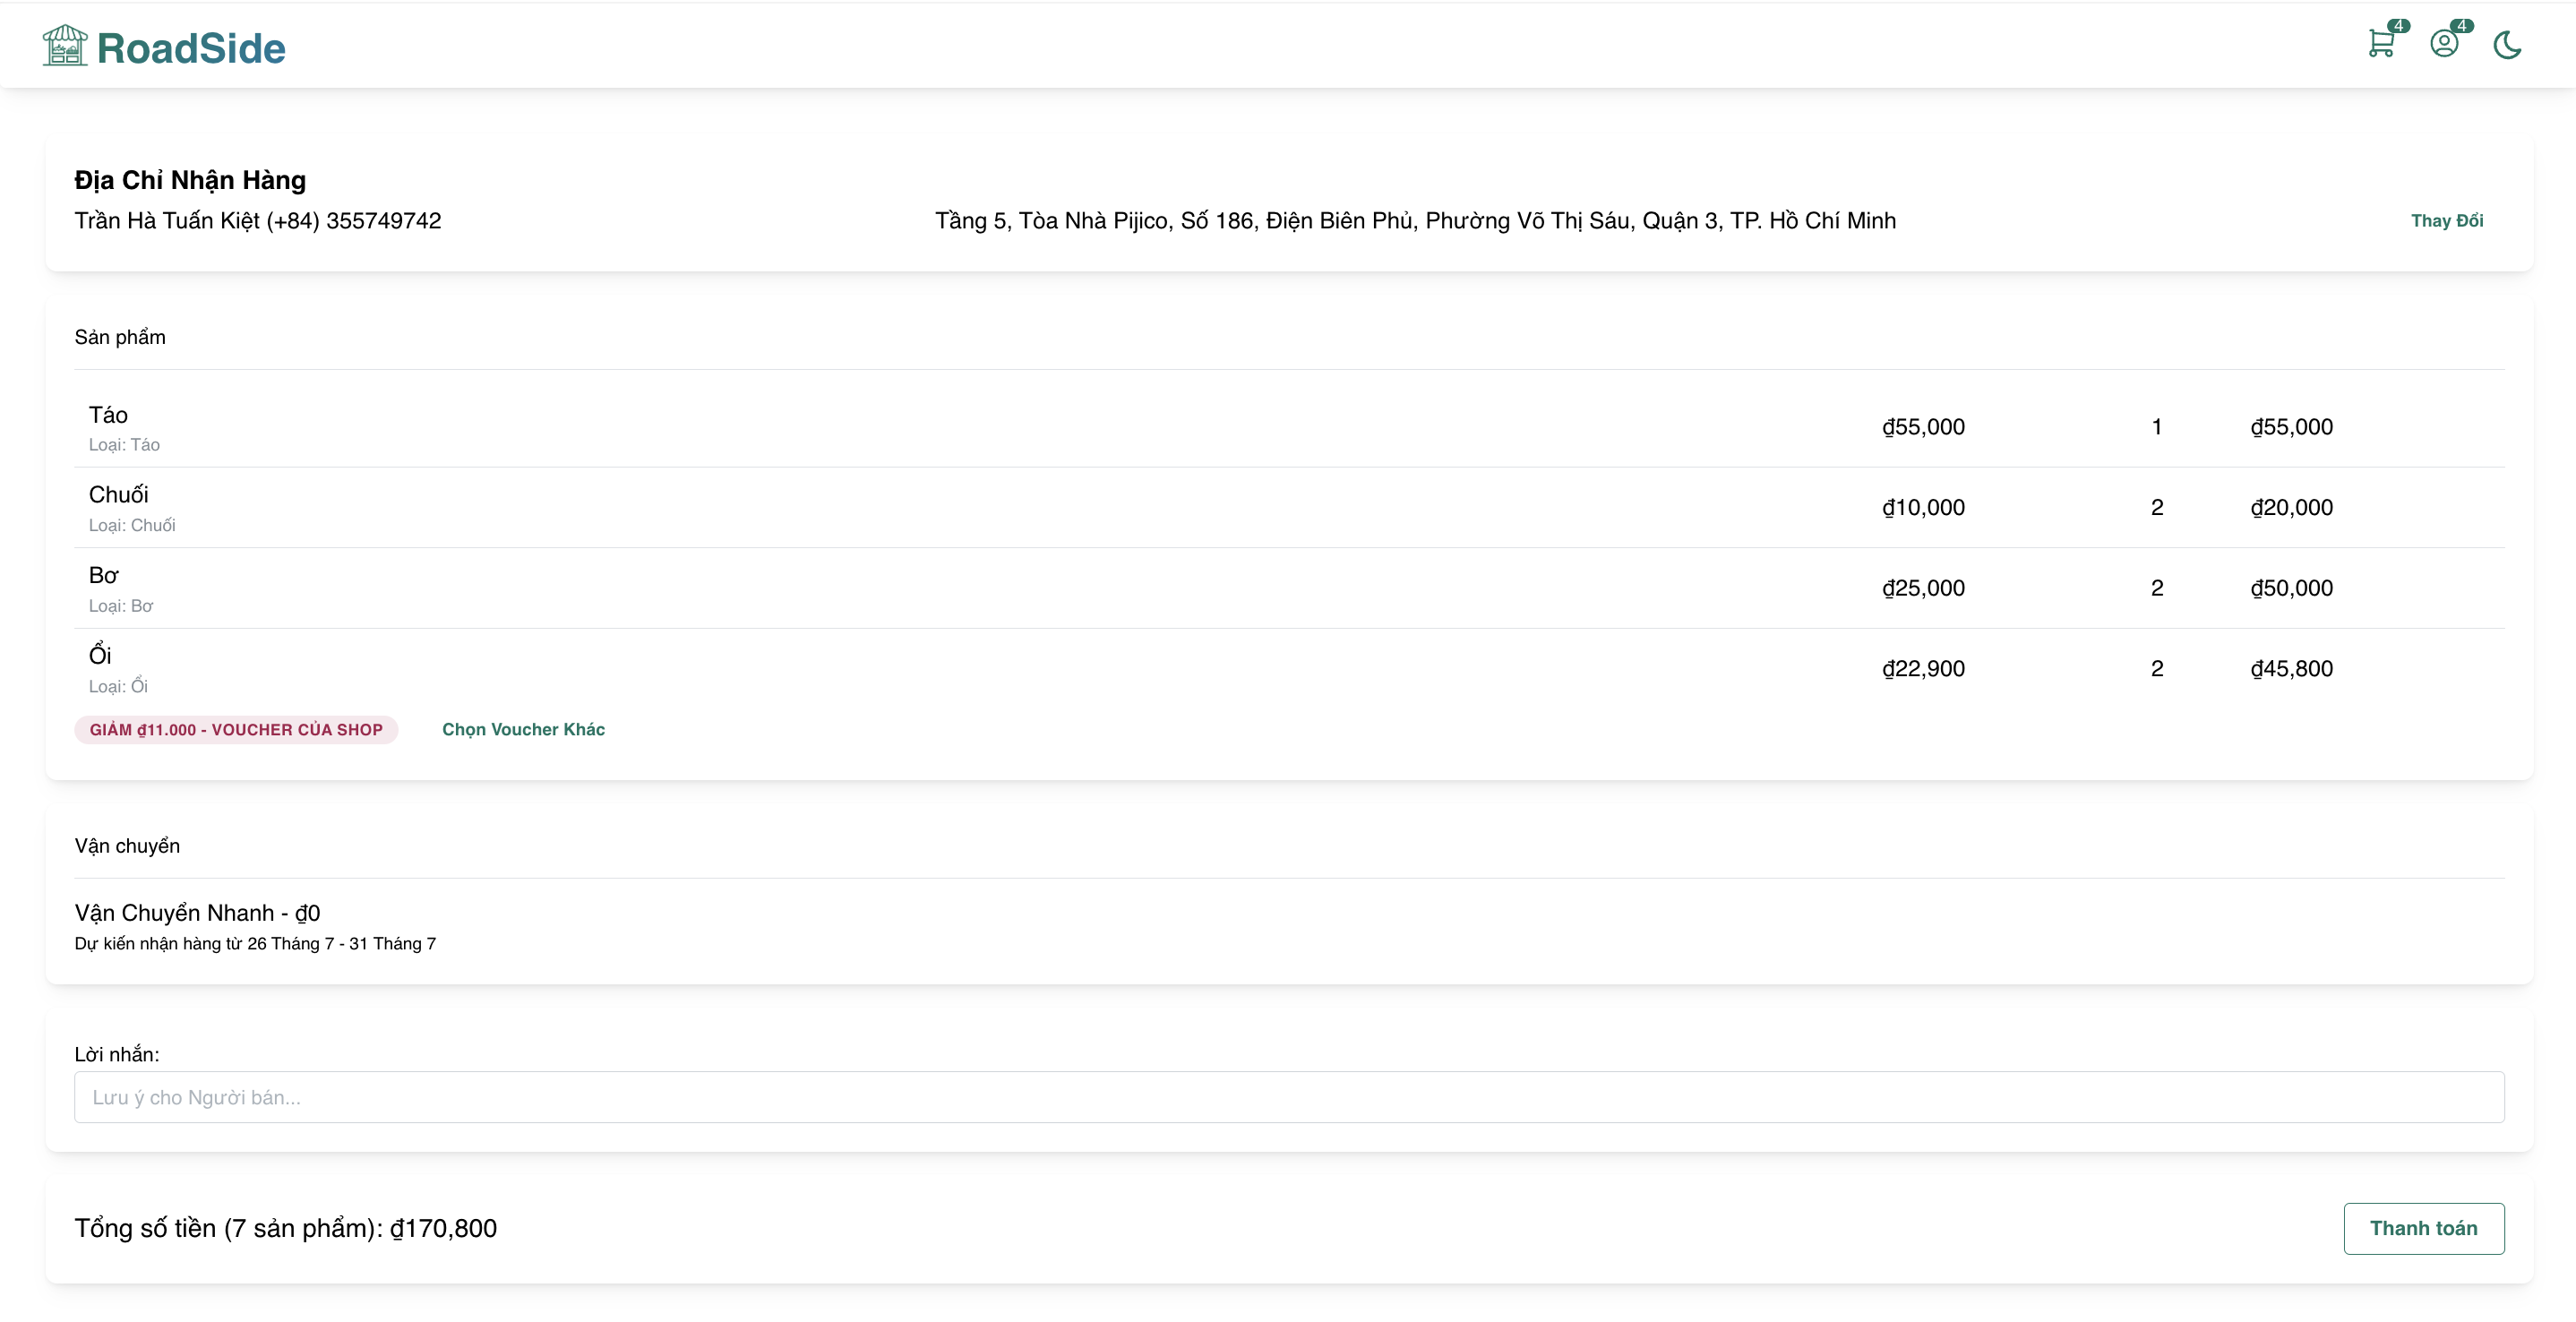
\includegraphics[scale=0.3] {Images/UI/orderform.png}
        \end{center}
        \caption{Form xác nhận đơn hàng}
    \end{figure}
Sau khi tiến hành đặt hàng và thanh toán thành công sẽ hiện thông báo đặt hàng thành công.
\subsection{Chỉnh sửa thông tin cá nhân}
Sau khi đăng nhập, người dùng có thể nhấn vào biểu tượng hình người trên thanh header để truy cập trang thông tin người dùng. Đây là nơi mà người dùng có thể quản lý và cập nhật thông tin cá nhân của họ. Trang này cung cấp cho người dùng một giao diện để xem và chỉnh sửa thông tin cá nhân, giúp tạo ra trải nghiệm cá nhân hóa cho khách hàng.

    \begin{figure}[H]
        \centering
        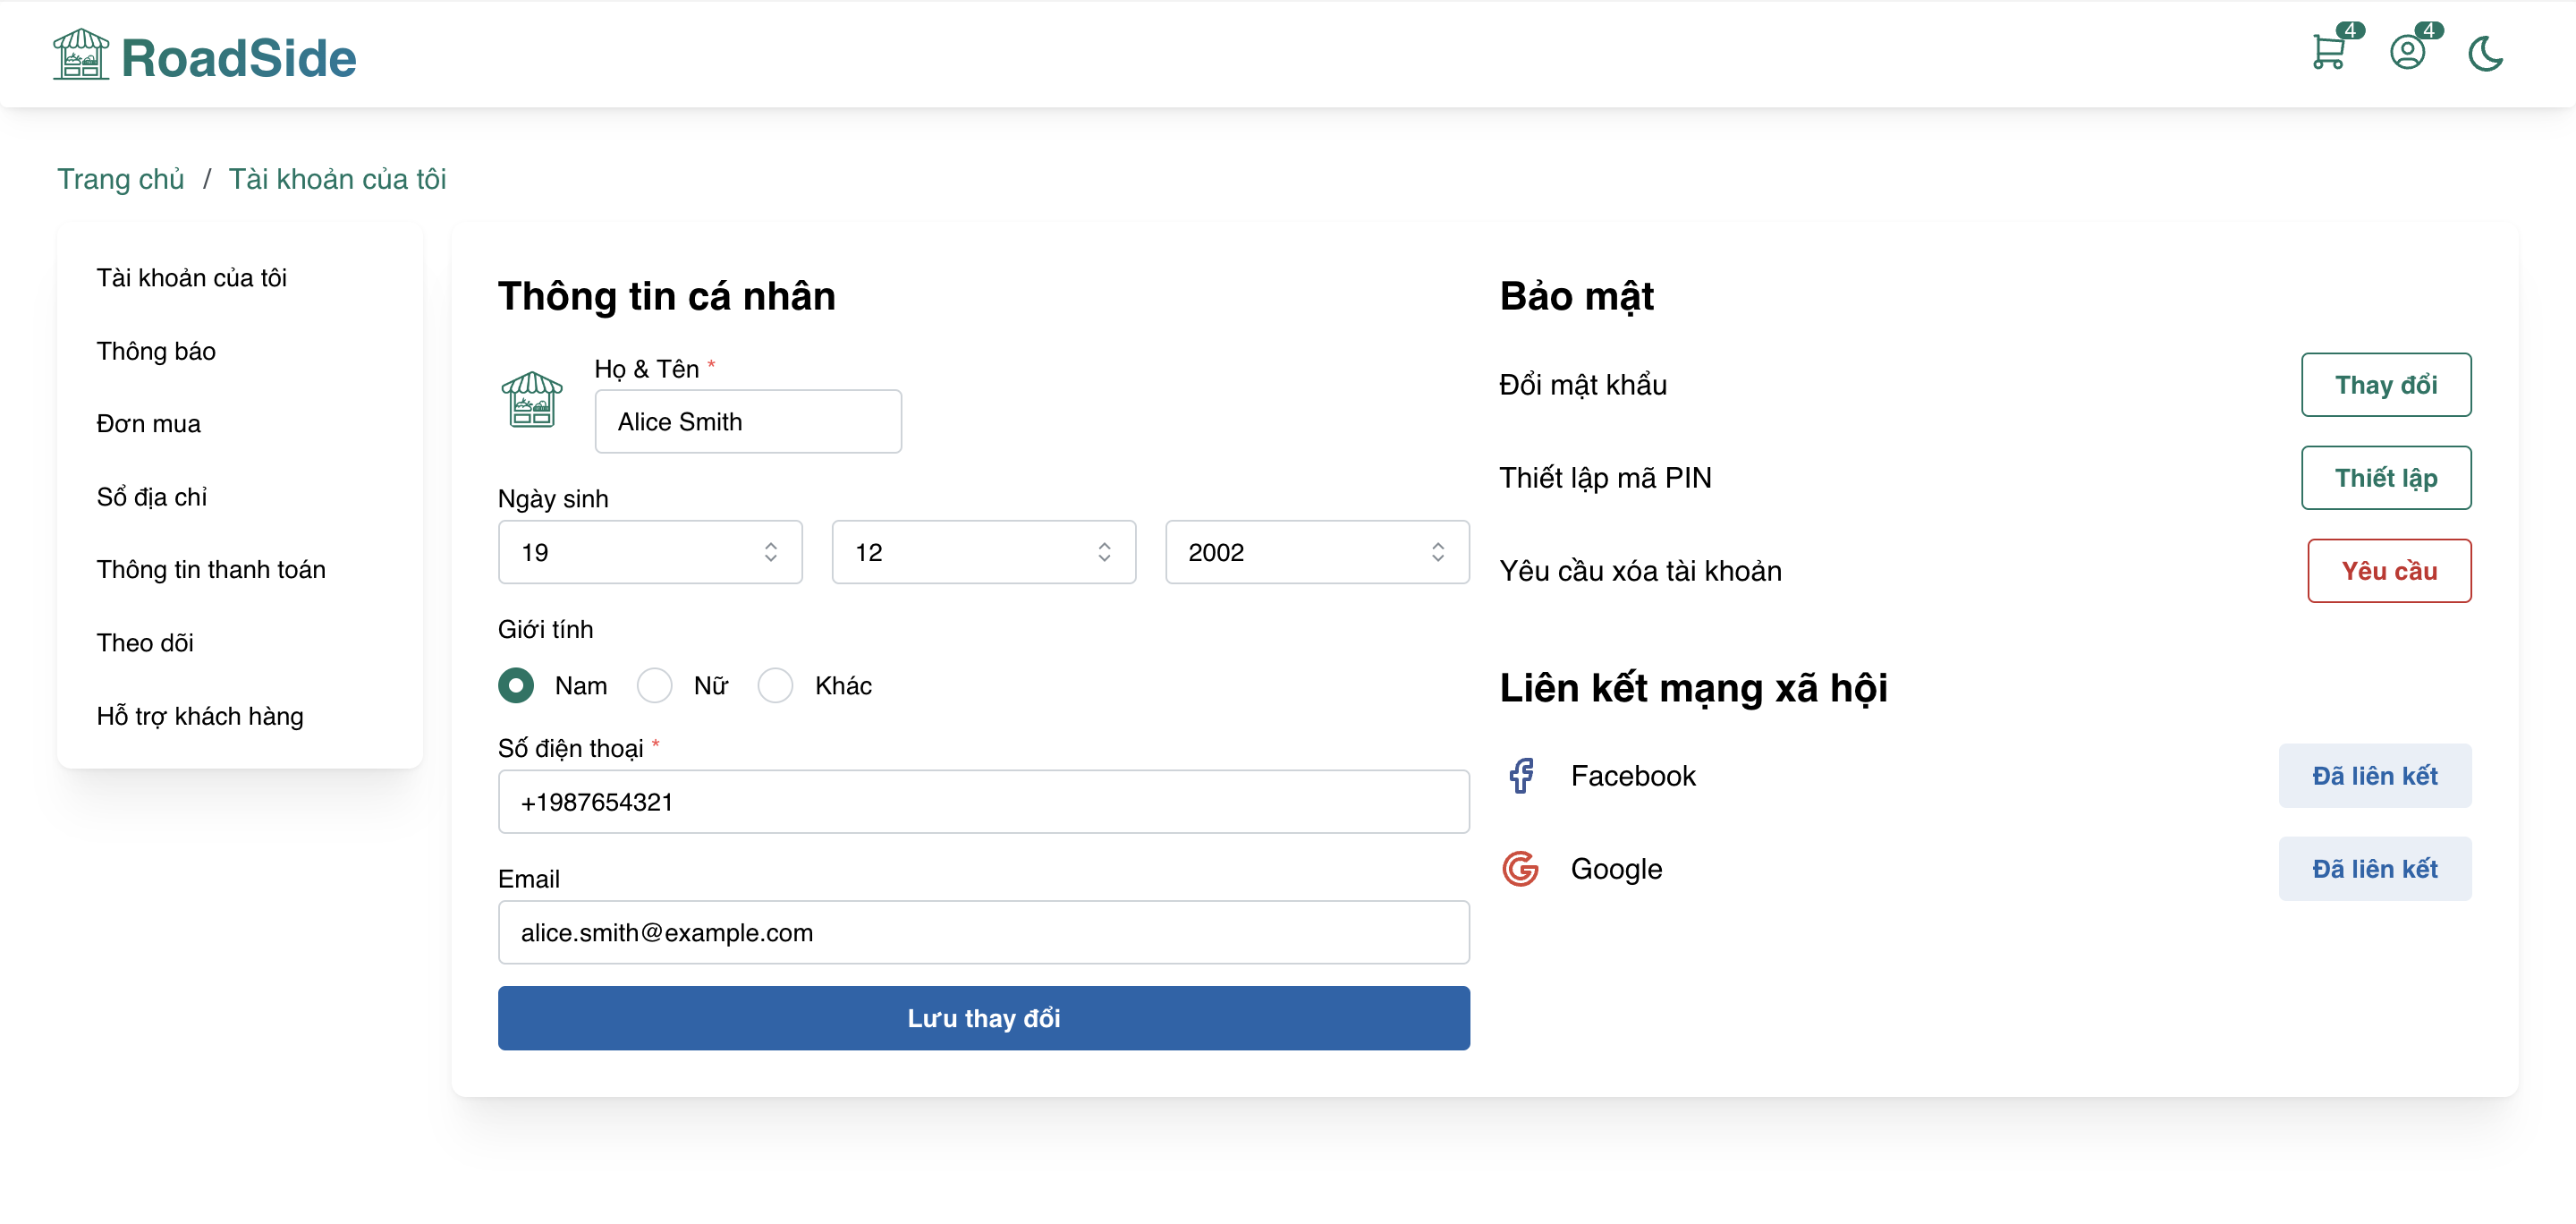
\includegraphics[scale=0.3] {Images/UI/info profile.png}
        \vspace{1em}
        \caption{Trang thông tin người dùng}
    \end{figure}
Trang thông tin người dùng cũng cung cấp khả năng thay đổi mật khẩu. Điều này cho phép người dùng cập nhật mật khẩu của mình một cách an toàn và bảo mật.

Người dùng cũng có thể thiết lập nhiều địa chỉ cho tài khoản của mình.  

\begin{figure}[H]
    \centering
    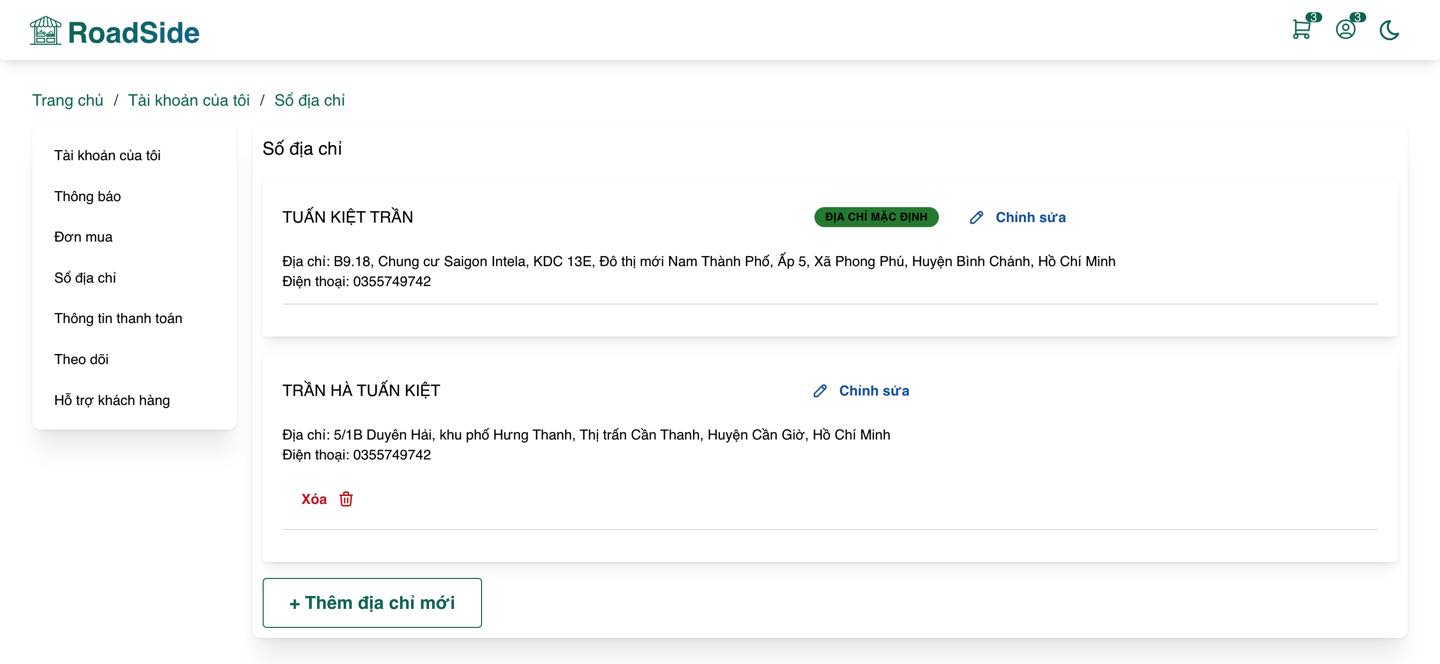
\includegraphics[scale=0.3] {Images/UI/address2.png}
    \vspace{1em}
    \caption{Địa chỉ người dùng}
\end{figure}
Với mỗi đơn hàng được đặt thành công, hệ thống sẽ gửi thông báo đến khách hàng và chủ cửa hàng, người dùng có thể xem thông báo chi tiết ở trang thông báo nằm trong phần thông tin người dùng này.
\begin{figure}[H]
    \centering
    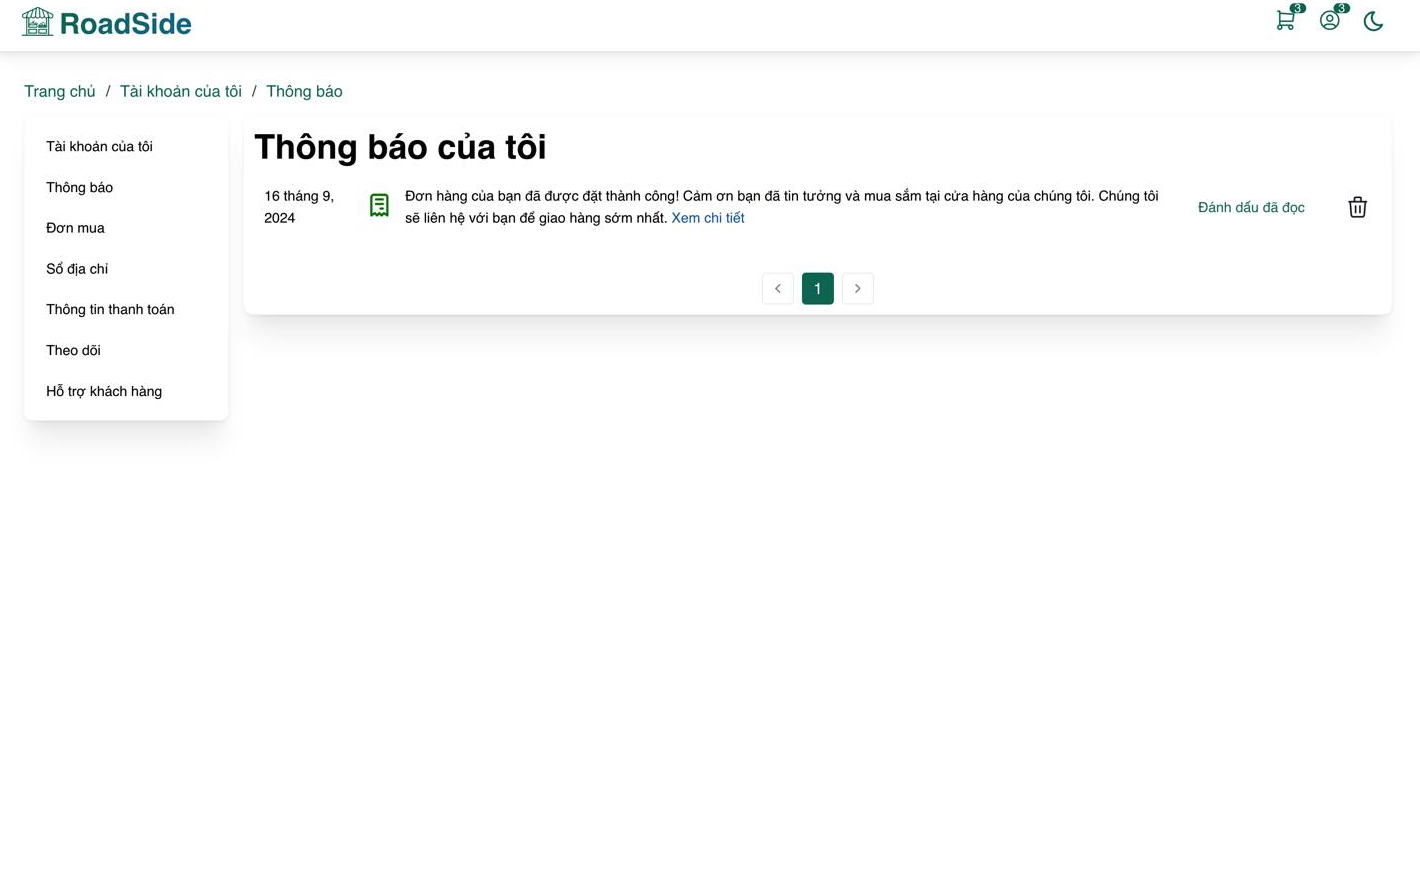
\includegraphics[width=\linewidth] {Images/UI/noti.png}
    \vspace{1em}
    \caption{Trang thông báo}
\end{figure}
Nếu có nhu cầu hỗ trợ từ hệ thống, người dùng cũng có thể truy cập thông qua nhóm trang thông tin người dùng này.
\begin{figure}[H]
    \centering
    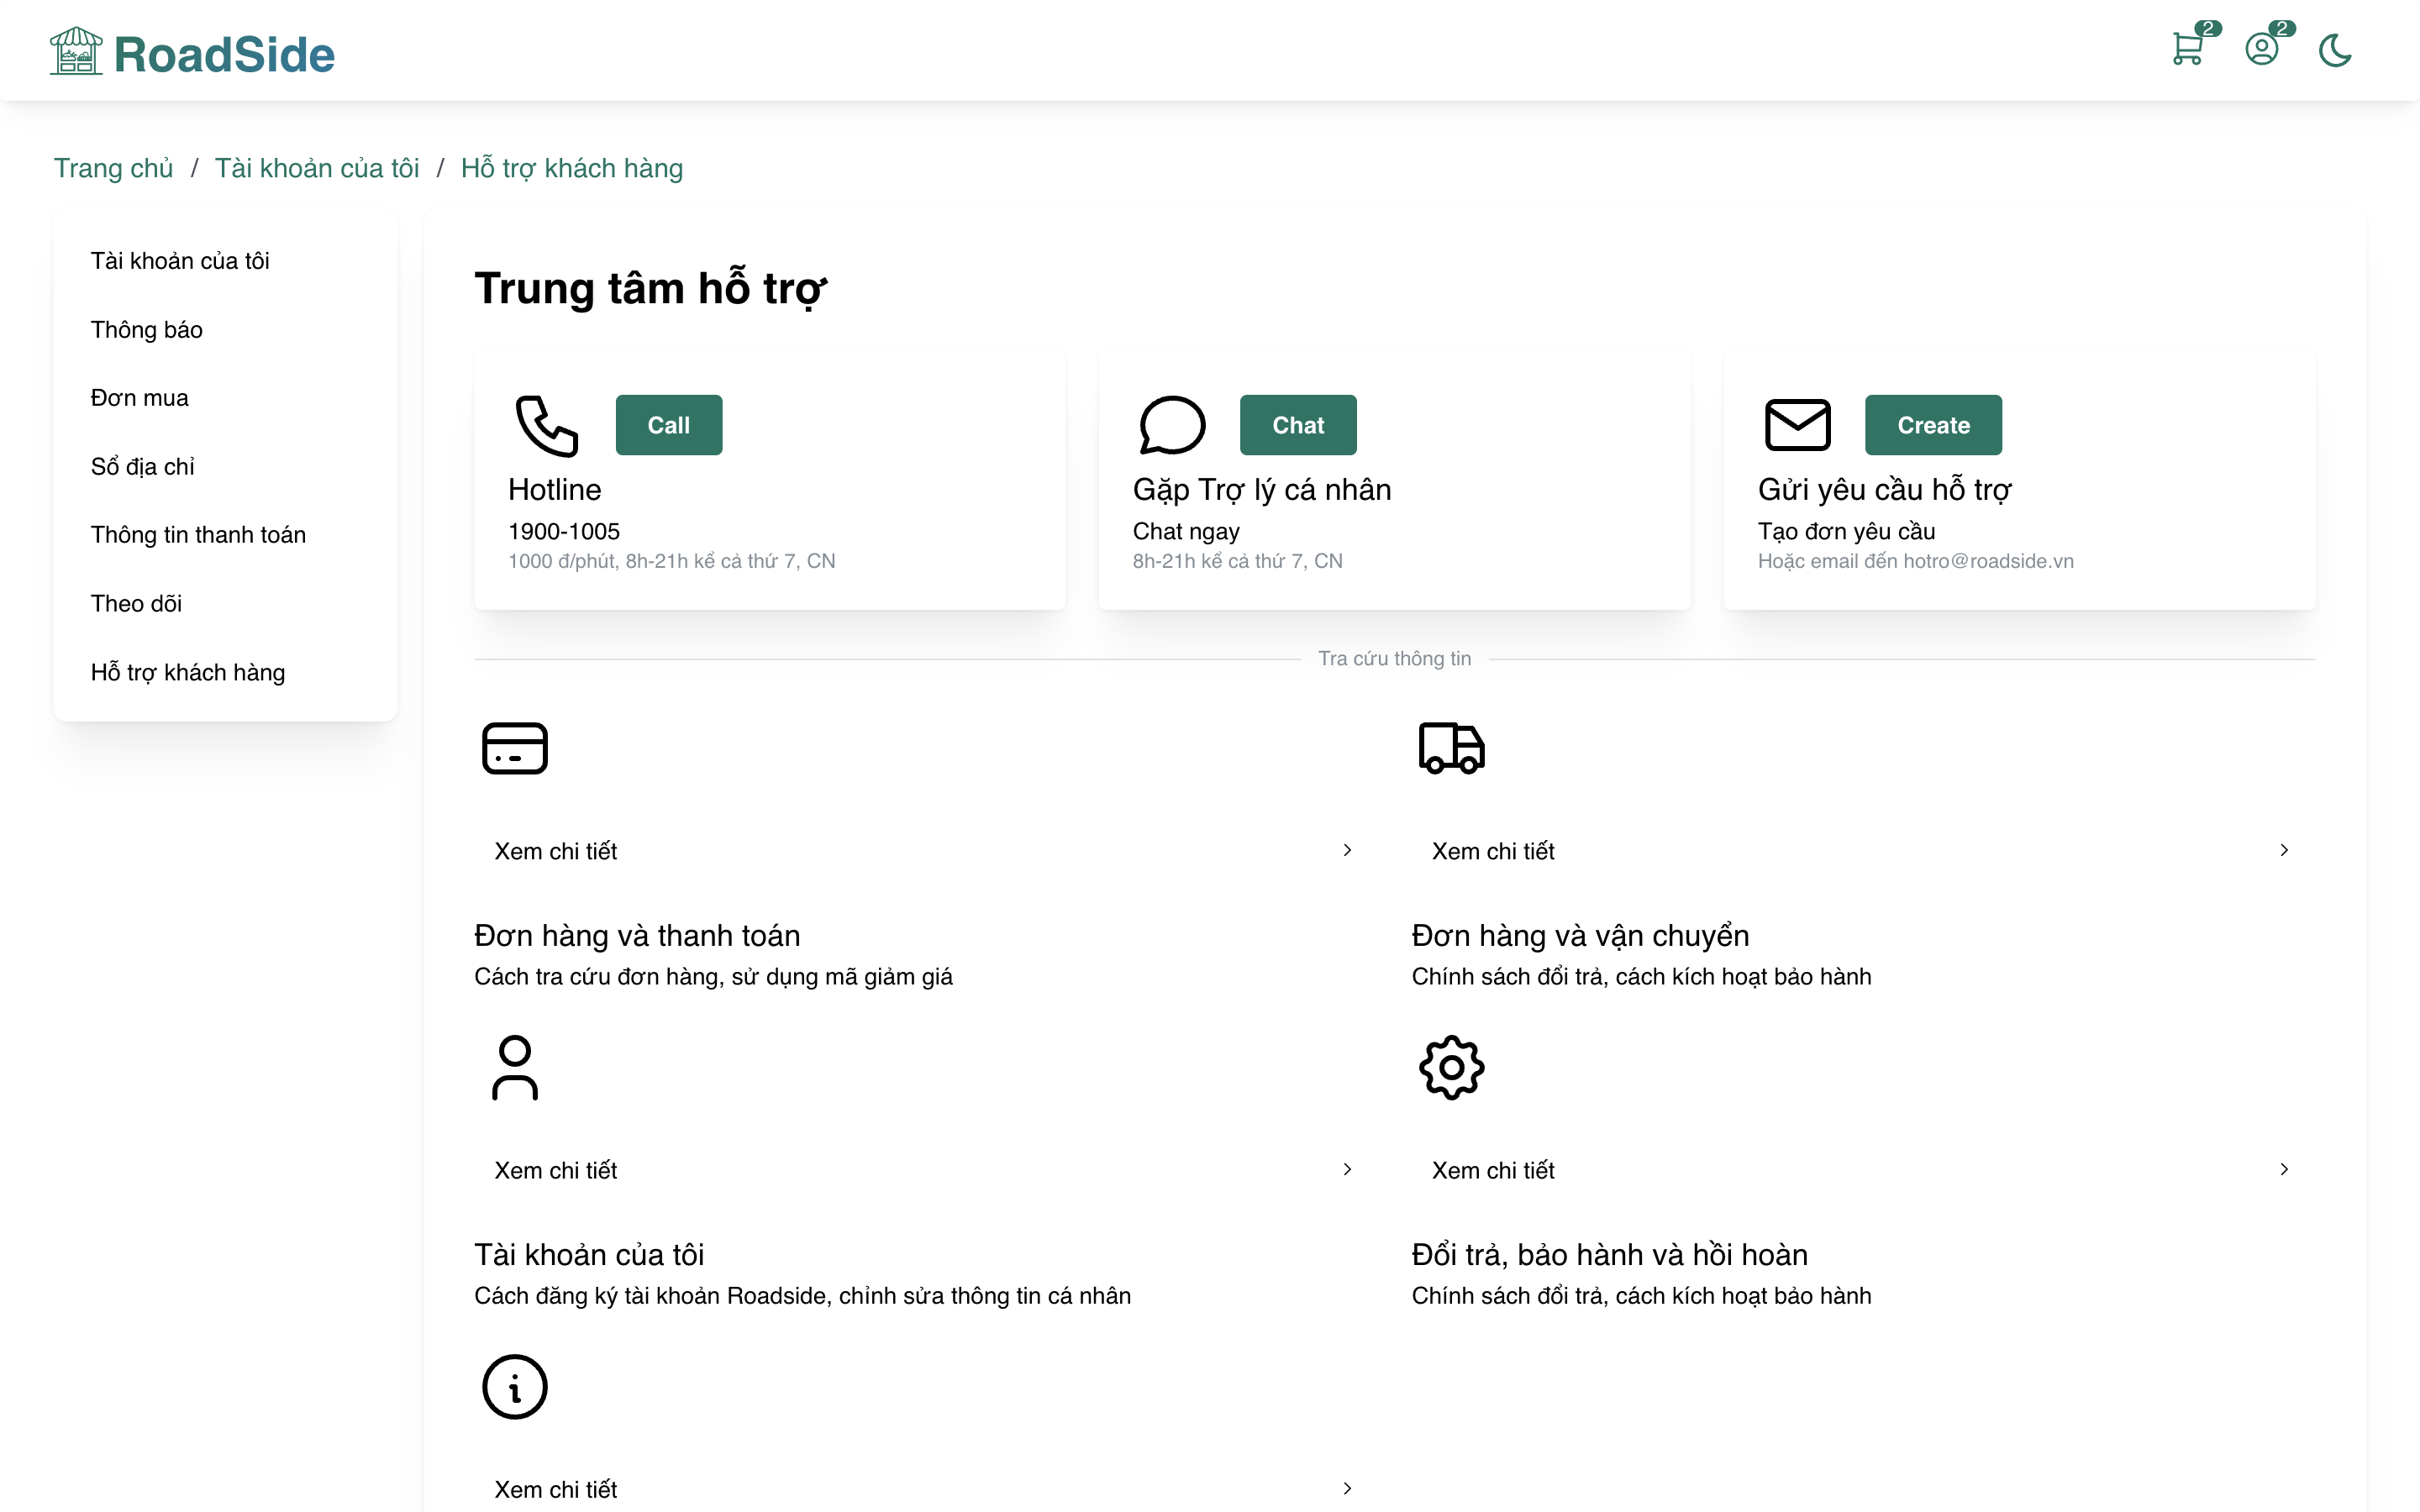
\includegraphics[width=\linewidth] {Images/UI/helpcenter.png}
    \vspace{1em}
    \caption{Trang hỗ trợ khách hàng}
\end{figure}
\subsection{Quản lý đơn đặt hàng}
Ở trang profile cũng cung cấp thông tin đơn hàng của người dùng, bao gồm các thông tin về đơn hàng đang trong quá trình vận chuyển hoặc các đơn đã hoàn thành trước đây như số đơn hàng, ngày đặt hàng, sản phẩm đã mua và trạng thái đơn hàng. Điều này giúp người dùng theo dõi và quản lý các đơn hàng của họ một cách thuận tiện.
    \begin{figure}[H]
        \centering
        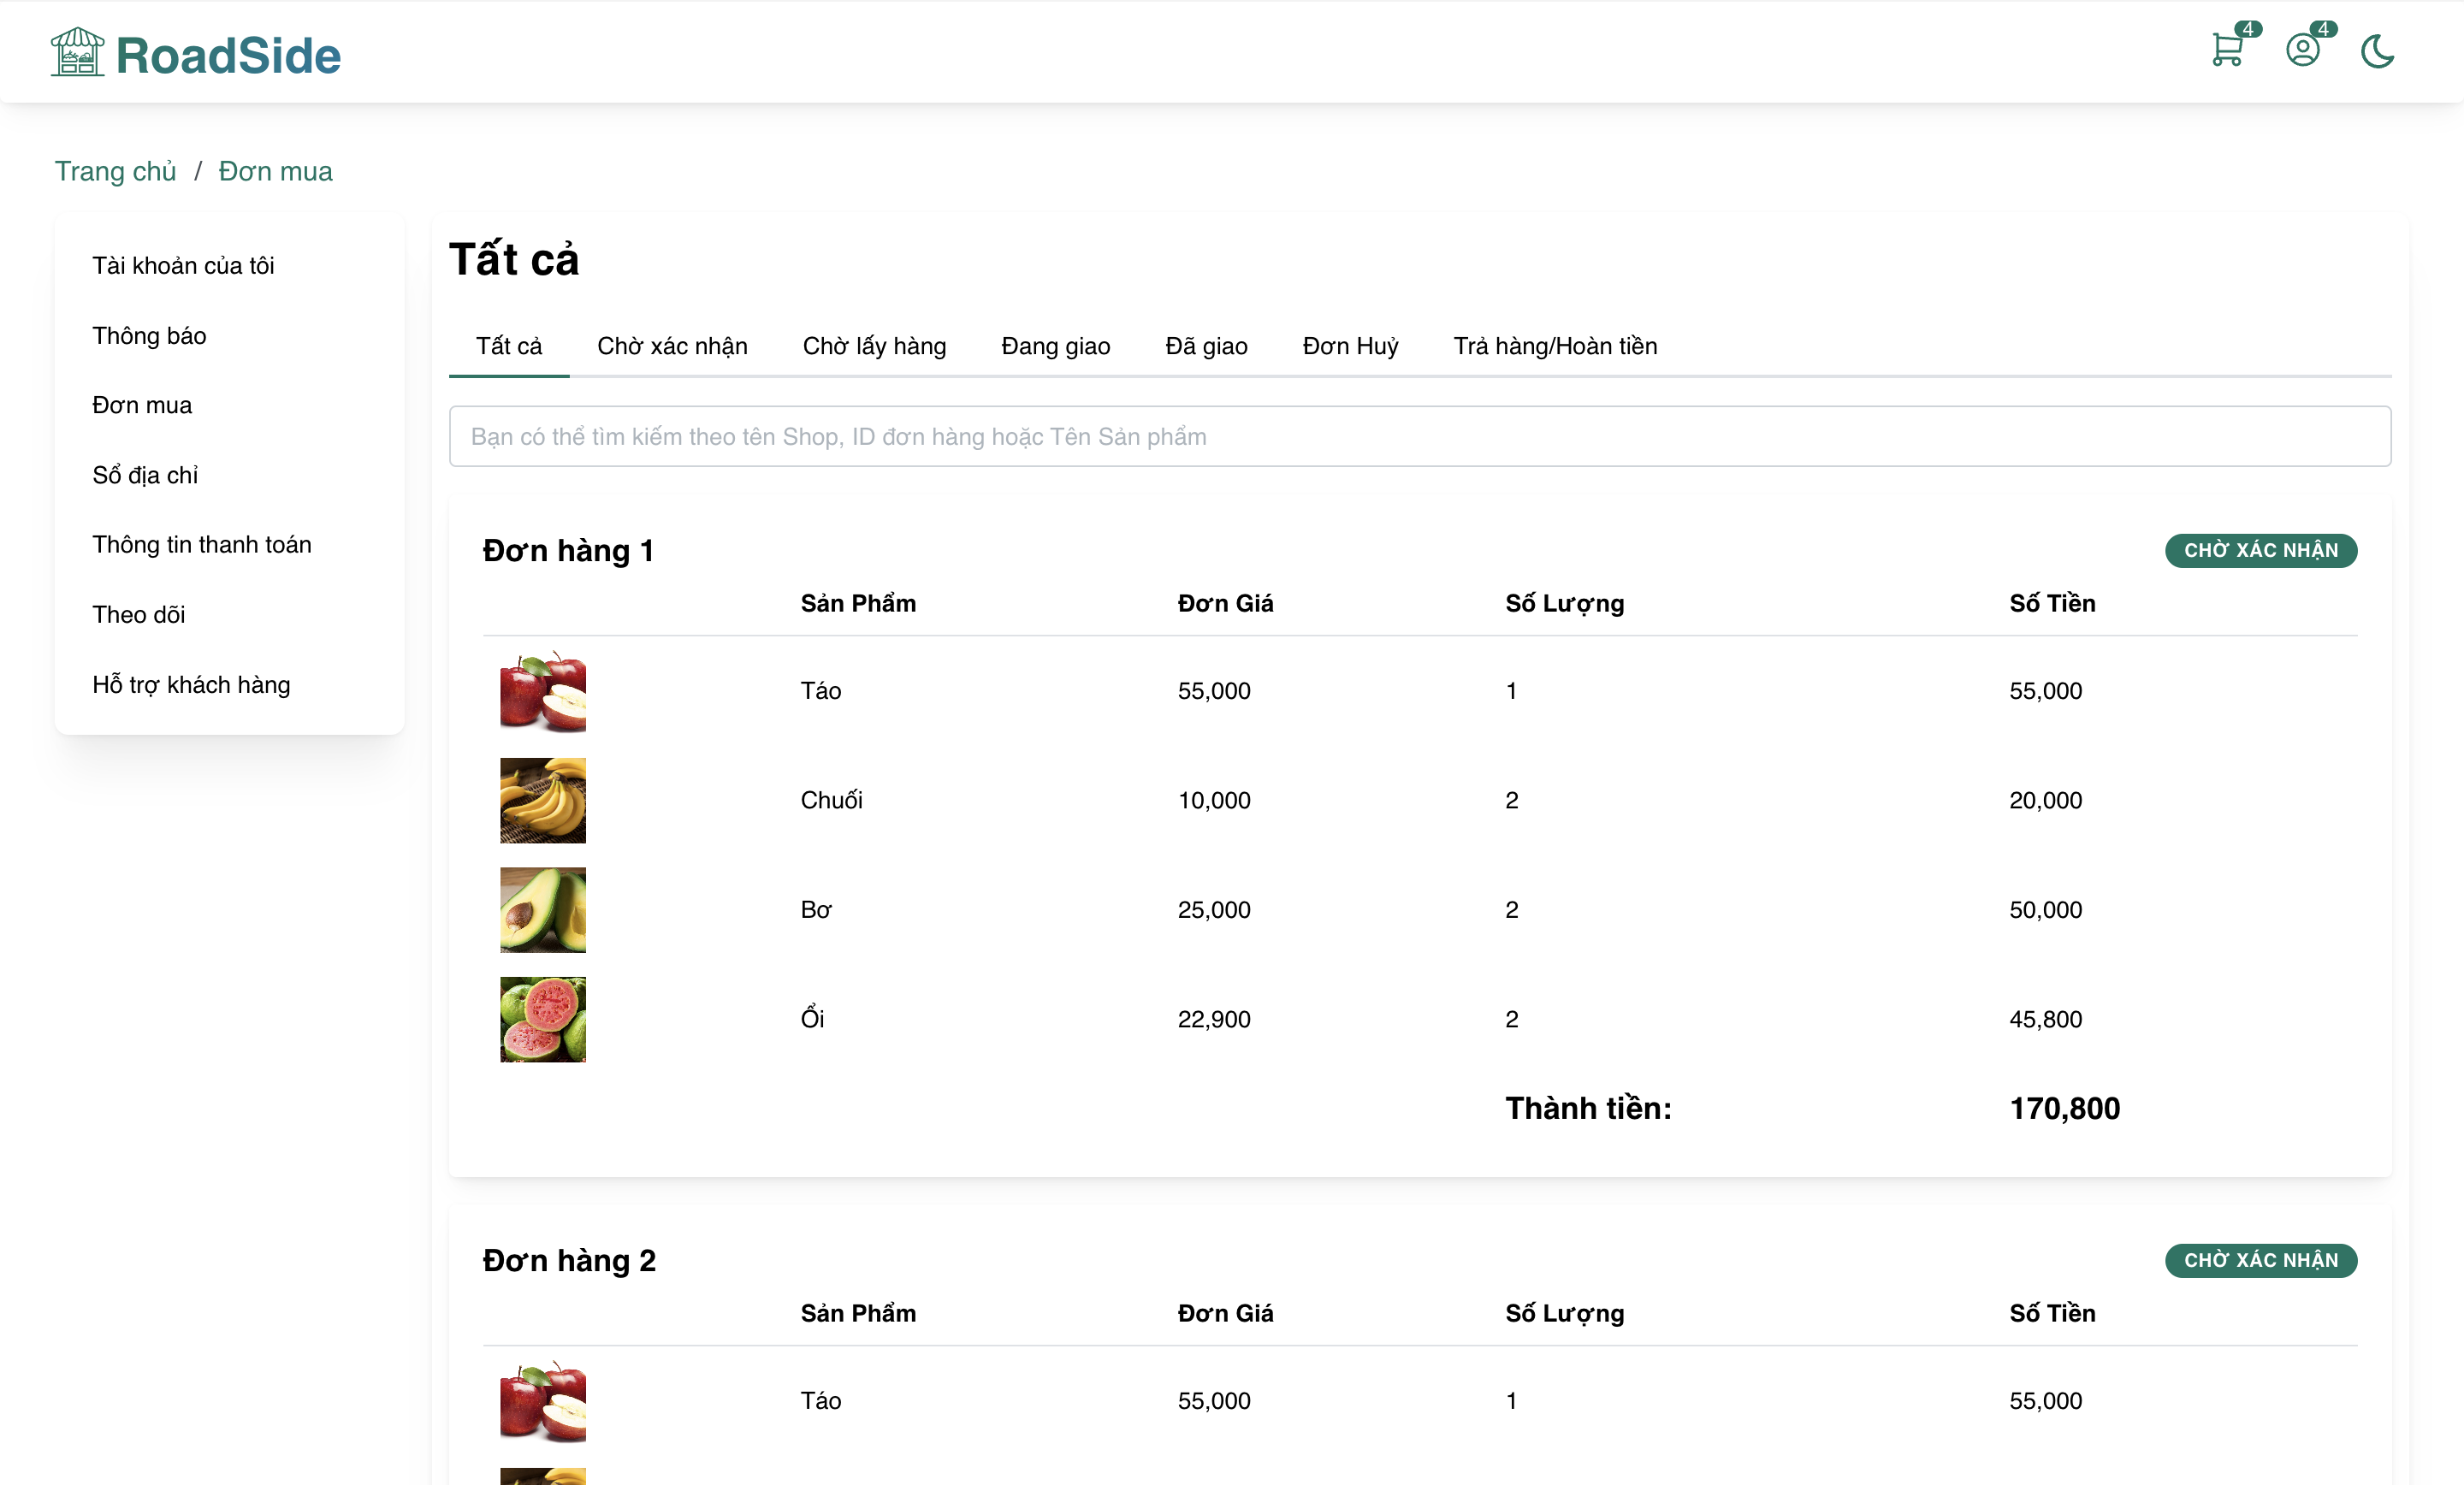
\includegraphics[width=\linewidth] {Images/UI/client order.png}
        \vspace{1em}
        \caption{Trang thông tin người dùng - Quản lý đơn hàng}
    \end{figure}
\subsection{Kênh cho chủ cửa hàng}
Mỗi tài khoản đều có thể tạo của hàng riêng cho mình, sẽ có một số trang riêng cho người dùng để quản lý cửa hàng và sản phẩm.
\begin{itemize}
    \item \textbf{Quản lý sản phẩm:}
    \begin{itemize}
        \item Tính năng quản lý sản phẩm cho phép chủ cửa hàng xem và quản lý các sản phẩm hiện có trong cửa hàng. Mỗi sản phẩm sẽ được hiển thị với các thông tin cơ bản như mã sản phẩm, tên, loại, giá, số lượng tồn kho và trạng thái hiện tại của sản phẩm. Ngoài ra, chủ cửa hàng cũng có thể xóa hay chỉnh sửa thông tin sản phẩm ở trang này.
        \begin{figure}[H]
            \centering
            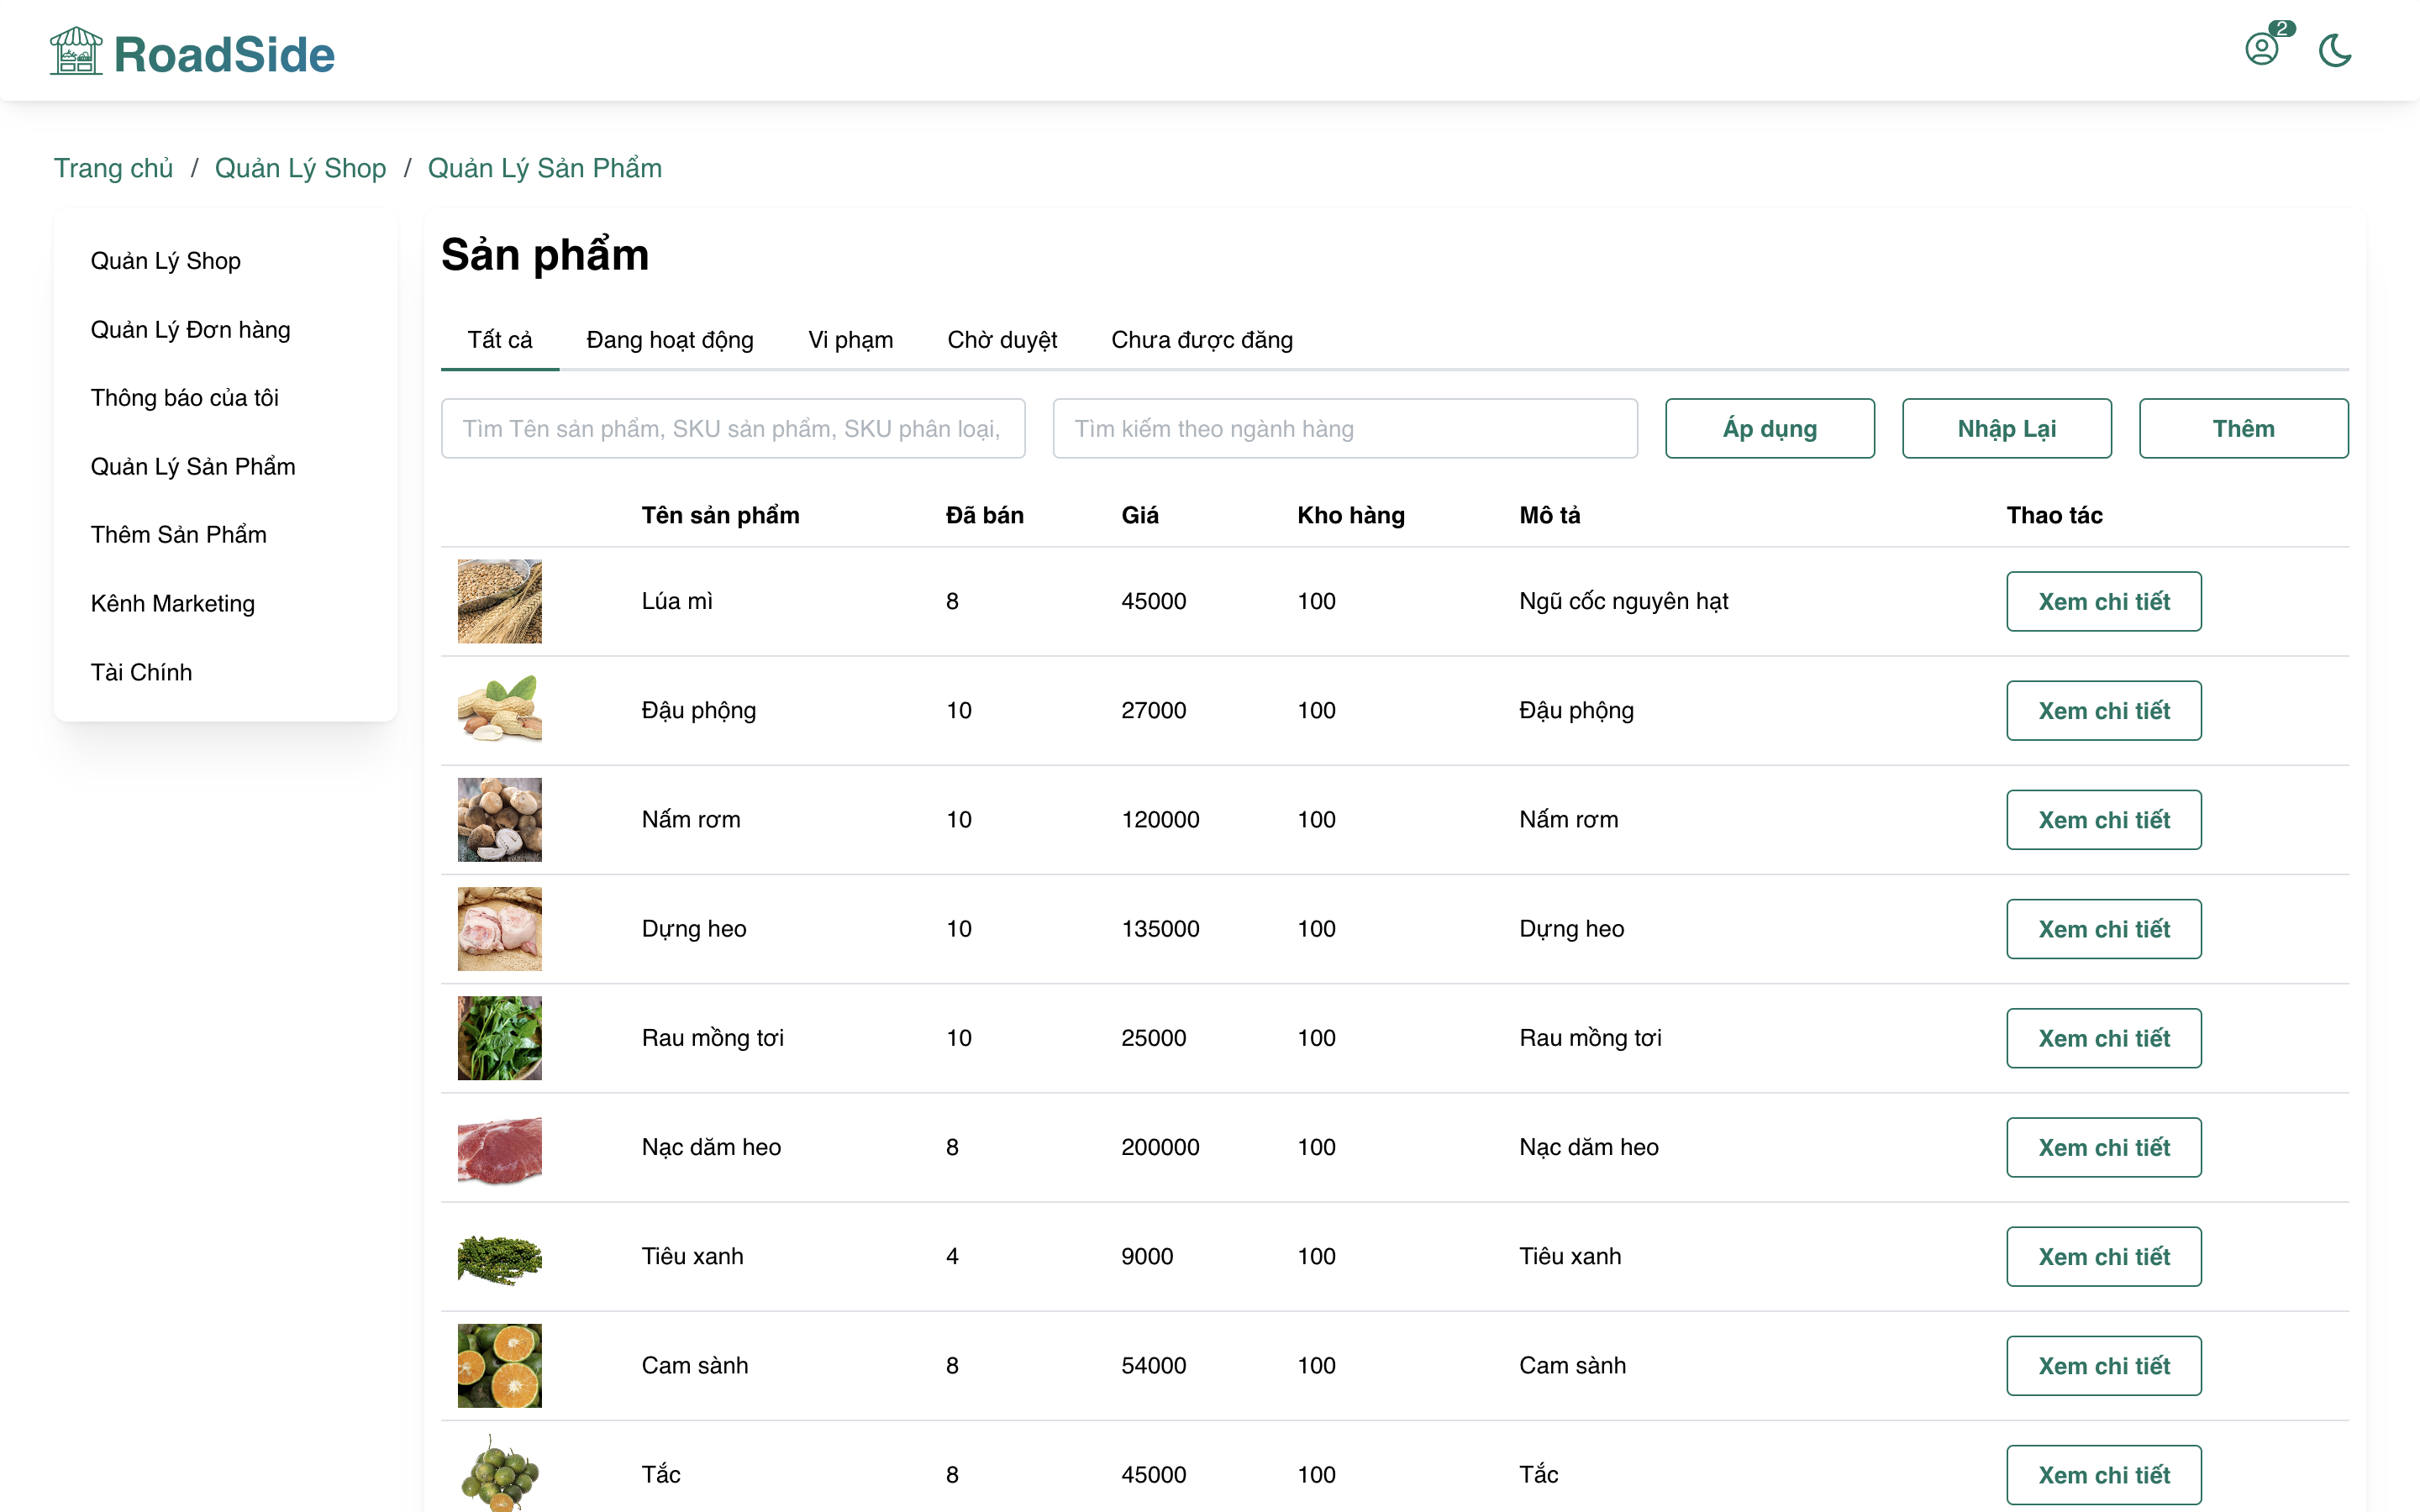
\includegraphics[width=0.95\linewidth] {Images/UI/shop_products.png}
            \vspace{1em}
            \caption{Quản lý sản phẩm}
        \end{figure}
        \item Chủ cửa hàng có thể lọc và tìm kiếm sản phẩm theo tên cũng như các đặc điểm khác.
        \item Thông tin của sản phẩm cũng có thể được chỉnh sửa ở đây.
    \end{itemize}
    \item \textbf{Thêm sản phẩm mới:} Chủ cửa hàng có thể thêm sản phẩm mới cho cửa hàng của mình thông qua tính năng này. Trong trang thêm sản phẩm, chủ cửa hàng sẽ phải điền một form với các trường thông tin chi tiết về sản phẩm như tên, hình ảnh, loại, mô tả,... 
        \begin{figure}[H]
            \begin{center}
            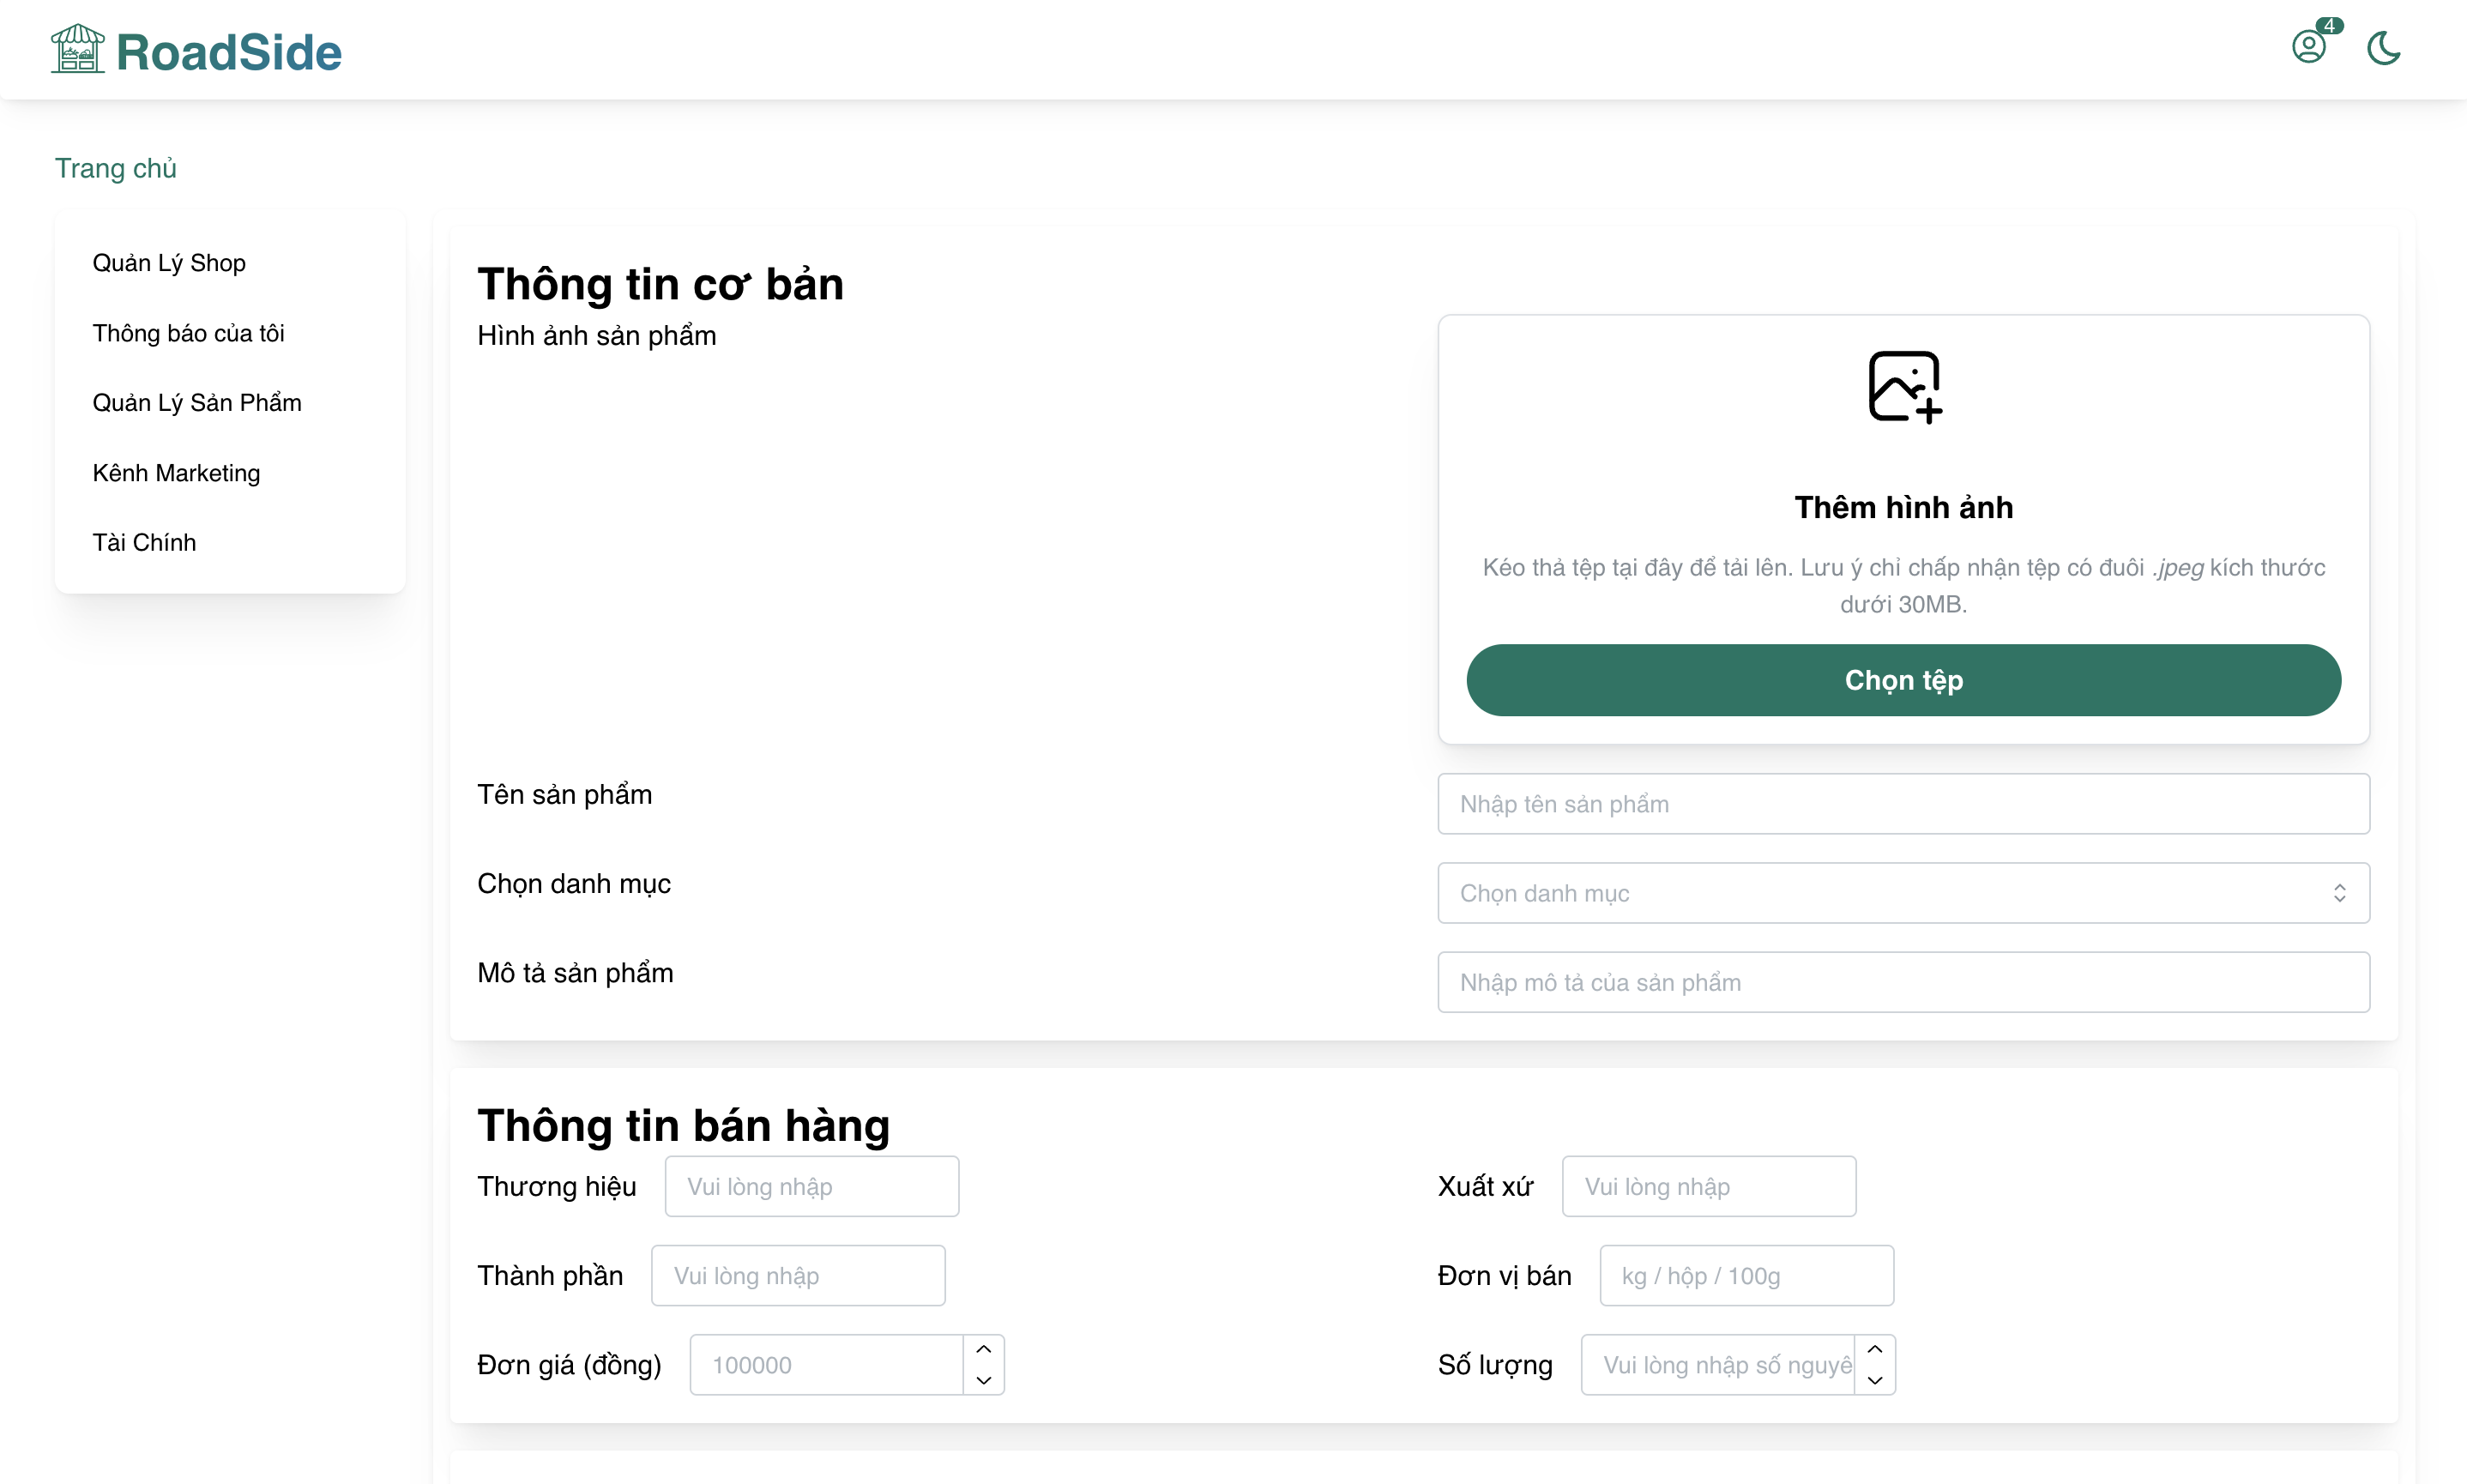
\includegraphics[width=\linewidth] {Images/UI/shop_addproduct.png}
            \end{center}
            \caption{Thêm sản phẩm mới}
        \end{figure}
    \item \textbf{Quản lý đơn hàng:} Trang này sẽ tổng hợp những đơn hàng đã được đặt thành công từ khách hàng và chủ cửa hàng có thể xem lại các đơn đó tại đây.
        \begin{figure}[H]
            \centering
            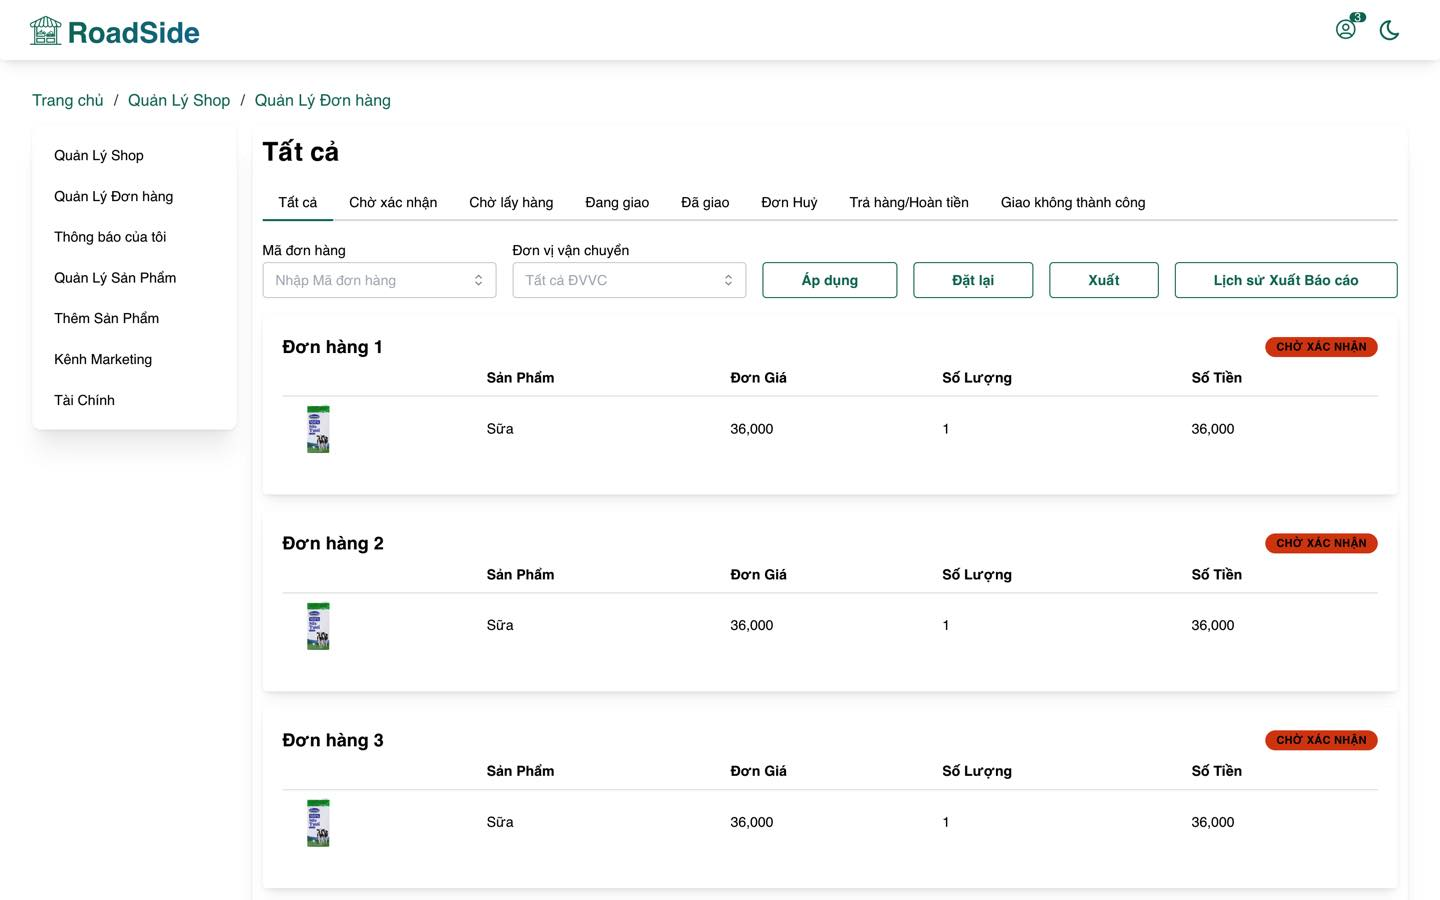
\includegraphics[width=\linewidth] {Images/UI/orders_shop.png}
        \end{figure}
        \begin{figure}[H]
            \centering
            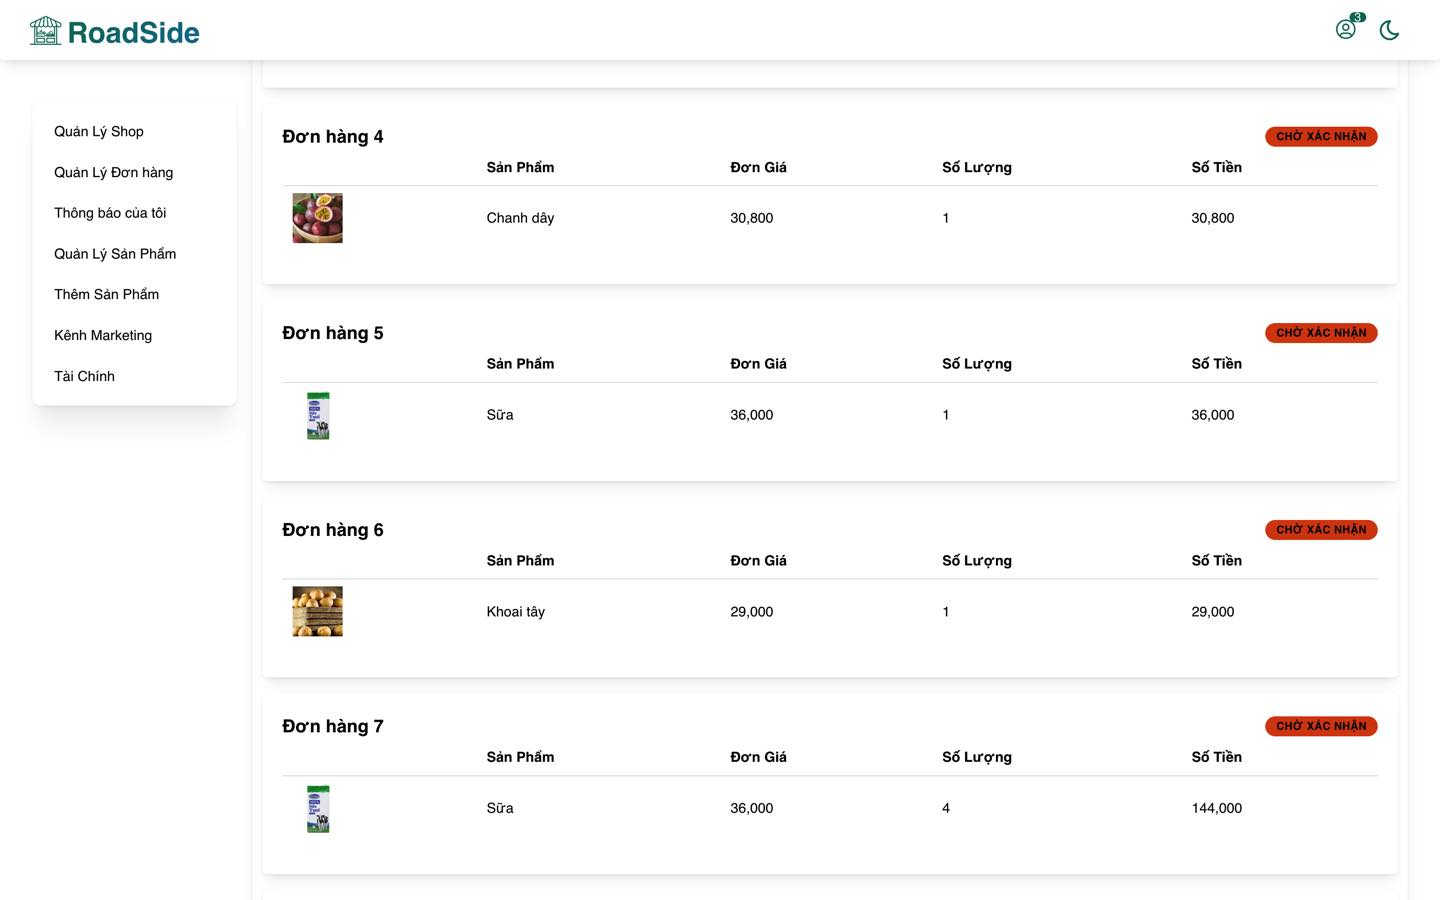
\includegraphics[width=\linewidth] {Images/UI/orders_shop2.png}
            \vspace{1em}
            \caption{Quản lý đơn hàng}
        \end{figure}
    \item \textbf{Quản lý đơn vị vận chuyển:} Chủ cửa hàng có thể chọn những đơn vị vận chuyển phù hợp với cửa hàng của mình tại đây.
        \begin{figure}[H]
            \centering
            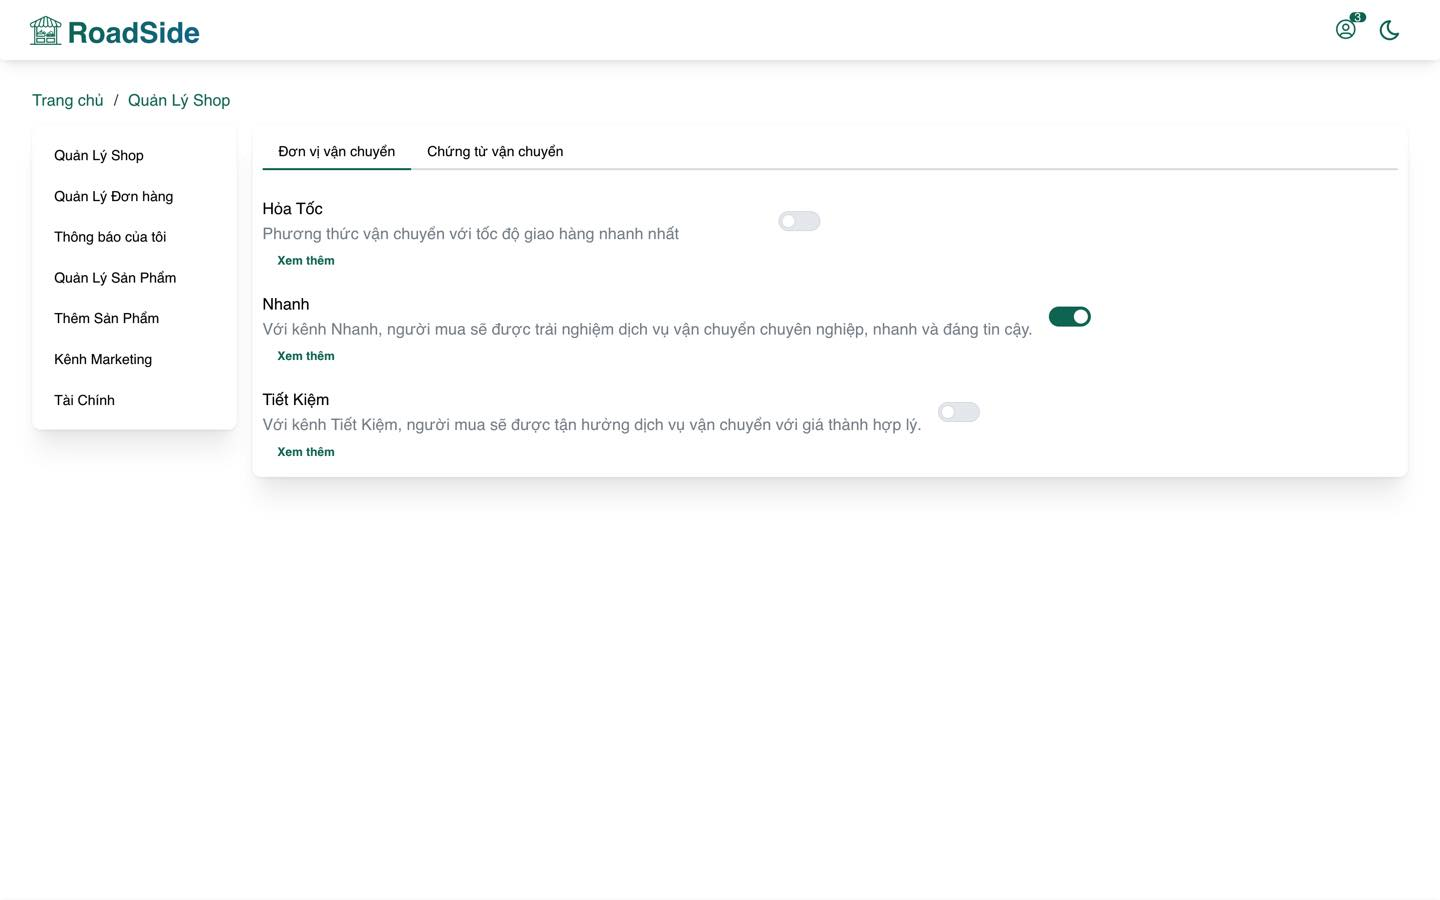
\includegraphics[width=\linewidth] {Images/UI/shop_shipping.png}
            \vspace{1em}
            \caption{Quản lý đơn hàng}
        \end{figure}
\end{itemize}

\subsection{Chế độ sáng - tối}
Ngoài ra trang web còn hỗ trợ chuyển đổi chế độ sáng - tối cho giao diện.
\begin{figure}[H]
    \centering
    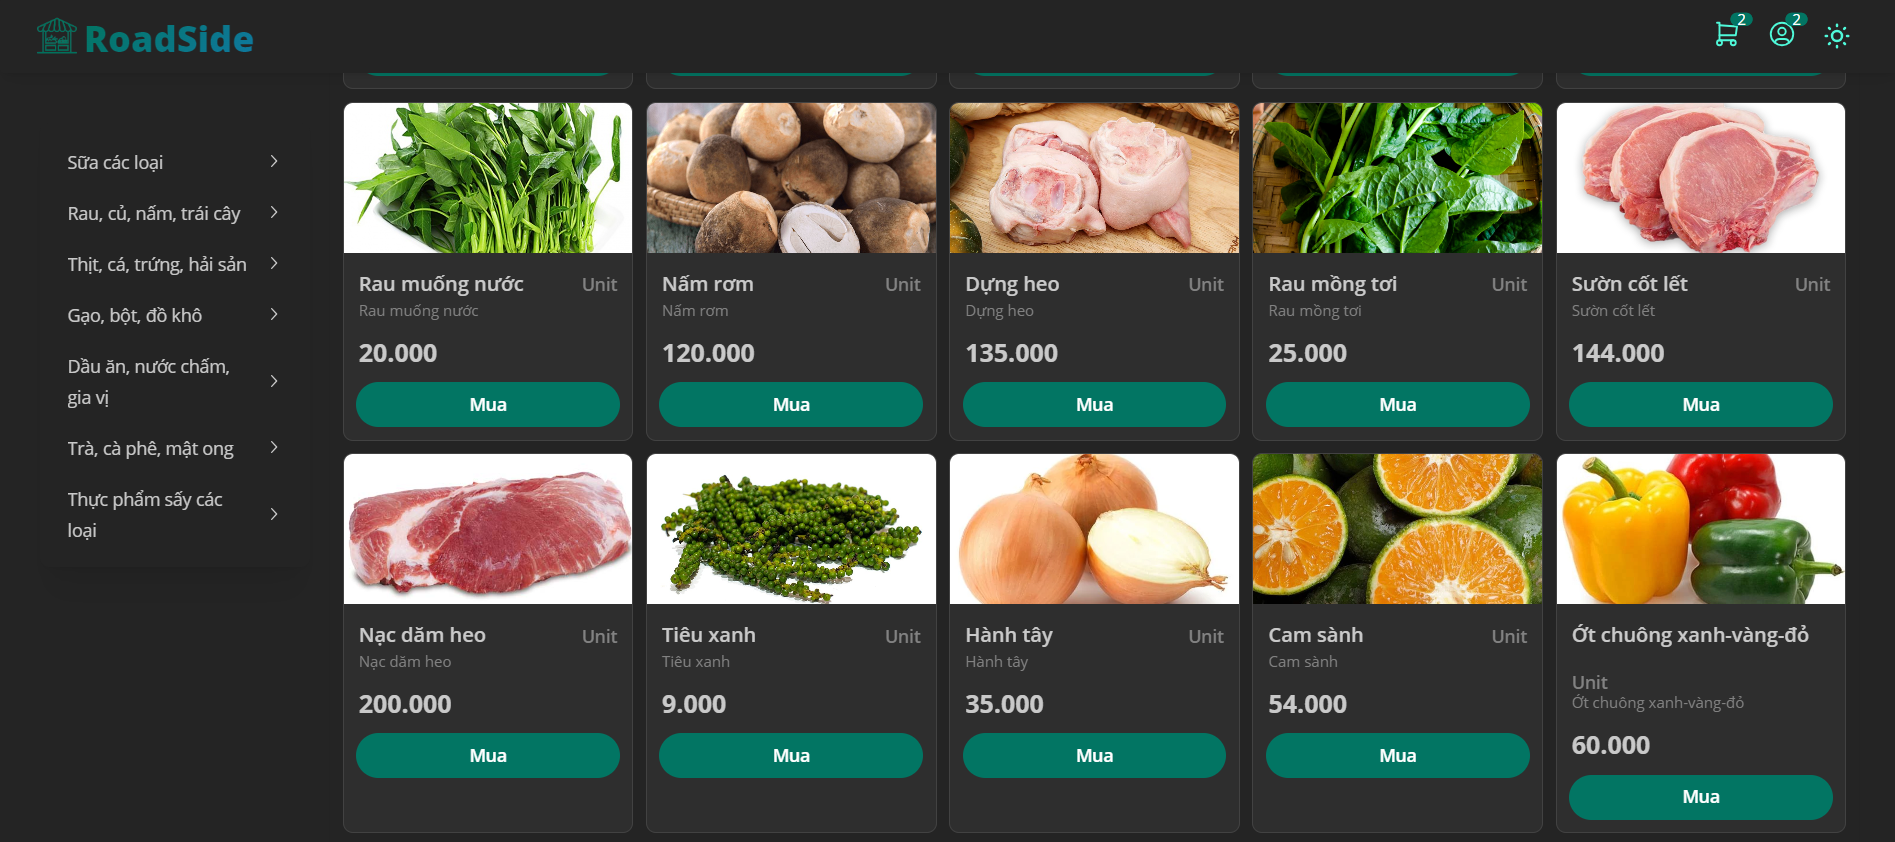
\includegraphics[width=0.95\linewidth] {Images/UI/darkmode1.png}
\end{figure}
\begin{figure}[H]
    \centering
    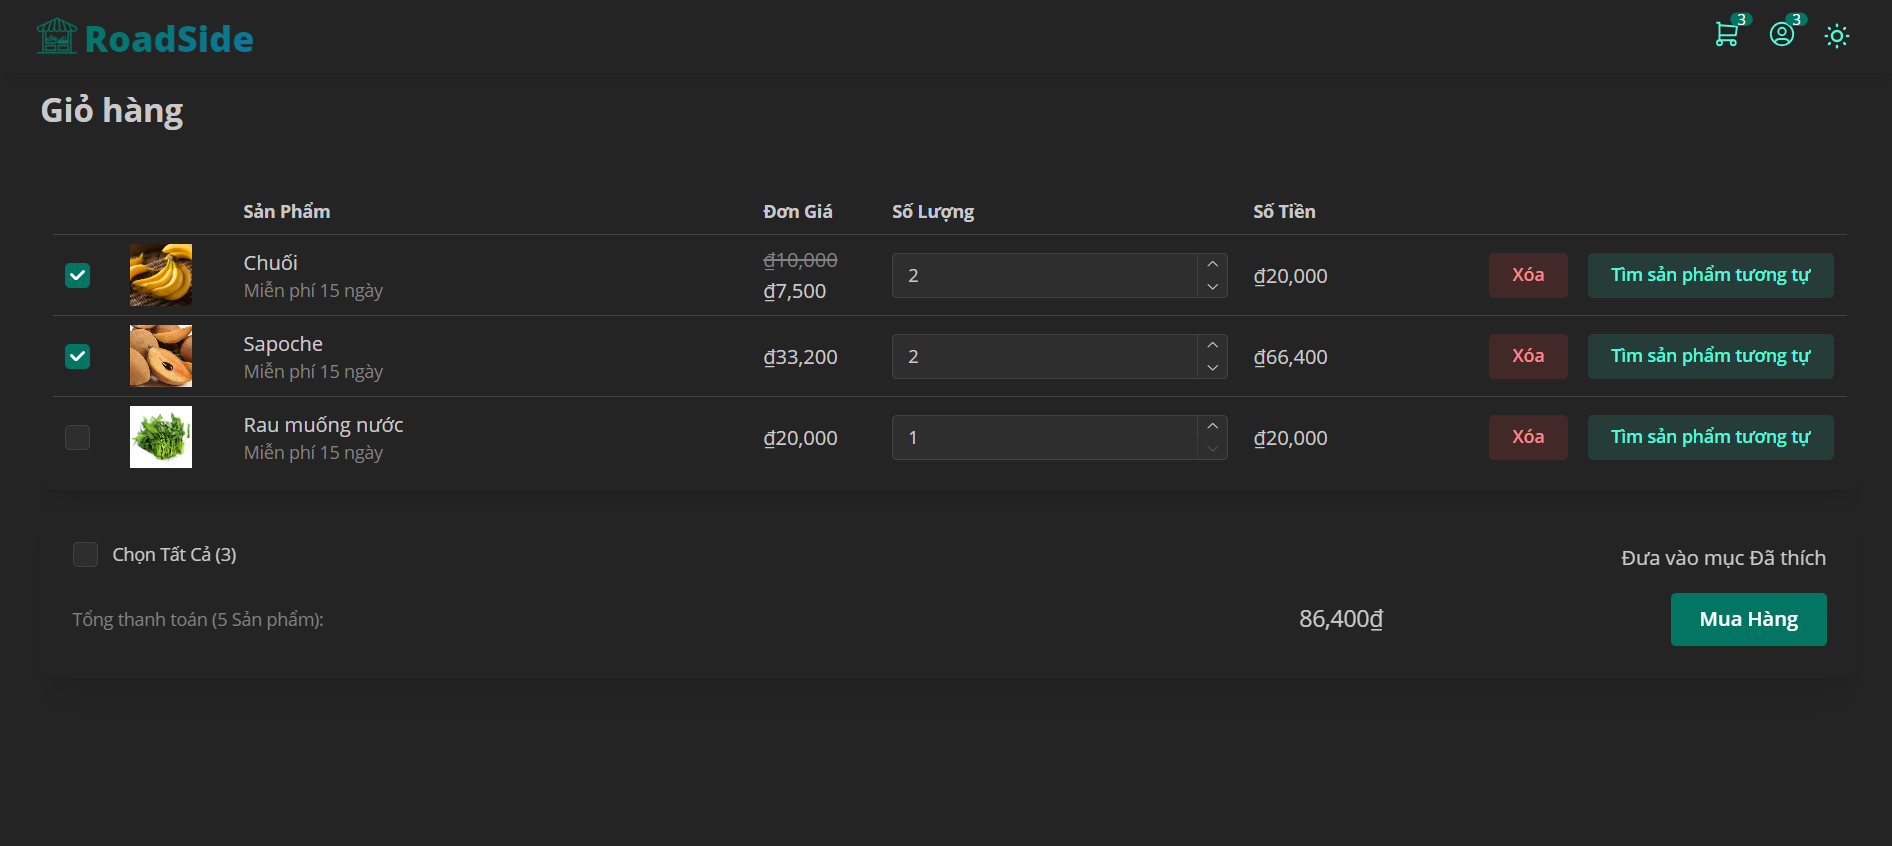
\includegraphics[width=0.95\linewidth] {Images/UI/darkmode2.png}
\end{figure}
\begin{figure}[H]
    \centering
    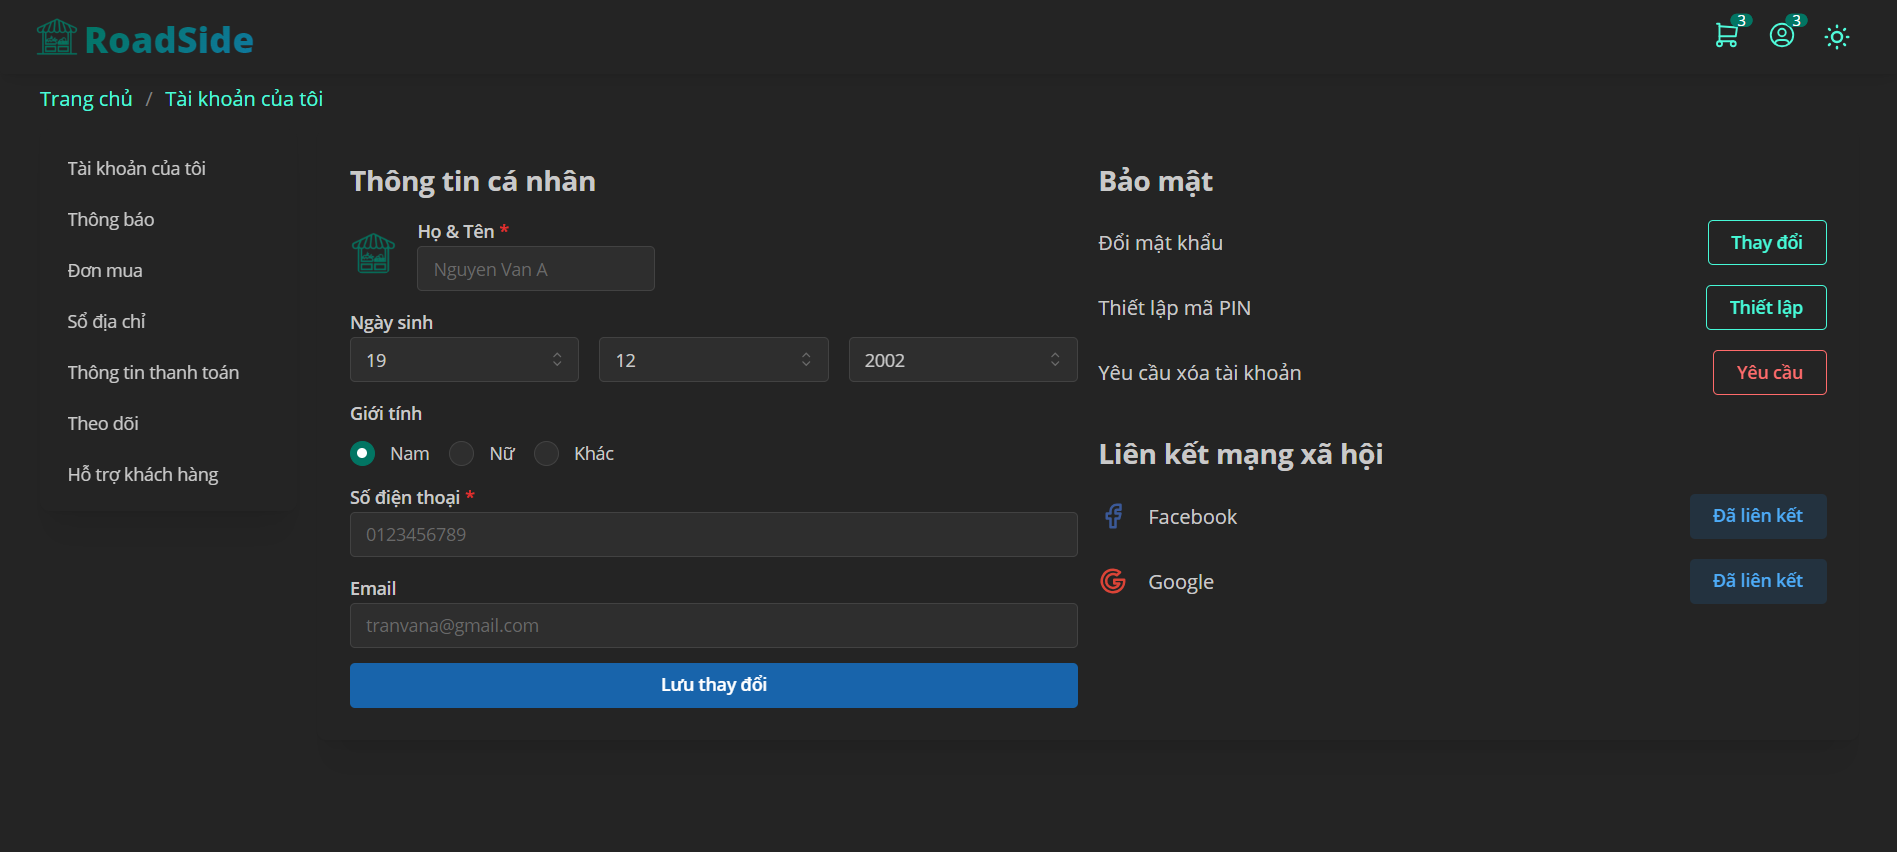
\includegraphics[width=0.95\linewidth] {Images/UI/darkmode3.png}
    \vspace{1em}
    \caption{Một số trang ở chế độ tối}
\end{figure}
\chapter{Tổng kết và hướng phát triển đề tài}
\label{Conclusion}

    \section{Tổng kết}
Trong quá trình nghiên cứu và triển khai dự án, nhóm chúng tôi đã đạt được các thành tựu quan trọng sau đây:
\begin{itemize}
    \item Nghiên cứu kỹ lưỡng và phân tích các sản phẩm tương tự trên thị trường để xác định các tính năng cần thiết cho hệ thống.
    \item Phân tích chi tiết các nghiệp vụ liên quan đến các đối tượng người dùng như chủ cửa hàng và khách hàng.
    \item Hoàn thành mô hình hóa cơ sở dữ liệu ở cấp độ khái niệm và luận lý.
    \item Thiết kế và mô tả chi tiết các usecase trong hệ thống thông qua sơ đồ usecase.
    \item Lựa chọn và áp dụng công nghệ phù hợp cho dự án:
        \begin{itemize}
            \item Sử dụng ASP.NET cho Back-end và Entity Framework cho tương tác cơ sở dữ liệu.
            \item Triển khai cơ sở dữ liệu trên PostgreSQL Database.
            \item Áp dụng thành công kiến trúc hệ thống theo hướng Clean Architecture để đảm bảo tính sạch sẽ, rõ ràng và dễ bảo trì của mã nguồn.
            \item Áp dụng các design pattern để thiết kế module, giúp các module trong hệ thống liên kết chặt chẽ và dễ dàng mở rộng.
            \item Kết nối chặt chẽ giữa hệ thống và cơ sở dữ liệu.
            \item Sử dụng Next.js cùng TypeScript và Mantine để phát triển giao diện người dùng.
        \end{itemize}
    \item Thiết kế kiến trúc mạng kết nối giữa người dùng và hệ thống, đảm bảo tính bảo mật và hiệu quả truyền tải dữ liệu.
    \item Triển khai hệ thống thành công trên Vercel, tăng cường khả năng truy cập và ổn định của hệ thống.
\end{itemize}

Chi tiết về quá trình hiện thực và các giao diện người dùng được trình bày cụ thể ở chương \ref{chap:Implementation}:
\hyperref[chap:Implementation]{\textcolor{blue}{Hiện thực}}.
    \section{Hướng phát triển}
$\indent$ Trong tương lai, chúng tôi kỳ vọng hệ thống này không chỉ được duy trì mà còn mở rộng các tính năng hiện tại, hướng tới các mục tiêu sau:
    \begin{itemize}
        \item Tối ưu hóa trải nghiệm người dùng bằng cách thiết kế giao diện thân thiện, đẹp mắt, và dễ sử dụng.
        \item Mở rộng phương thức thanh toán, tích hợp thêm các giải pháp thanh toán mới để tăng cường sự tiện lợi và an toàn cho người tiêu dùng và nhà cung cấp.
        \item Cải thiện an ninh mạng, áp dụng các biện pháp bảo mật mạnh mẽ để đảm bảo an toàn cho dữ liệu và thông tin cá nhân của người dùng.
        \item Phát triển chức năng đánh giá và nhận xét sản phẩm, qua đó xây dựng một cộng đồng mua sắm minh bạch và tin cậy.
        \item Khám phá và áp dụng Trí Tuệ Nhân Tạo (AI) và Học Máy (Machine Learning) để cải tiến trải nghiệm mua sắm, cụ thể là:
        \begin{itemize}
            \item Phân loại và lọc sản phẩm tự động, giúp người dùng dễ dàng tìm kiếm và lựa chọn.
            \item Phát triển các mô hình so sánh sản phẩm, đề xuất các lựa chọn thay thế phù hợp dựa trên giá, đánh giá và tính năng.
            \item Triển khai các mô hình gợi ý sản phẩm dựa trên lịch sử mua hàng và hành vi duyệt web của người dùng để cung cấp gợi ý cá nhân hóa.
        \end{itemize}
        \item Tích hợp tính năng gợi ý thông minh vào giao diện người dùng, giúp hiển thị các sản phẩm được đề xuất tùy theo hành vi tìm kiếm của từng người dùng.
    \end{itemize}

Những hướng phát triển này không chỉ nhằm mục đích nâng cao chất lượng trải nghiệm người dùng mà còn đảm bảo hệ thống "Sàn Thương Mại Điện Tử Nông Sản" không chỉ thích ứng linh hoạt với các biến động của thị trường mà còn vượt qua kỳ vọng của người dùng, từng bước hoàn thiện và phát triển.


\begin{thebibliography}{80}
    \bibitem{clean} \href{https://blog.cleancoder.com/uncle-bob/2012/08/13/the-clean-architecture.html}{\color{black}The Clean Architecture, Robert C. Martin (Uncle Bob), \\ https://blog.cleancoder.com/uncle-bob/2012/08/13/the-clean-architecture.html}

    \bibitem{design pattern} \href{https://refactoring.guru/design-patterns}{\color{black}Design Patterns, ©2014-2023 Refactoring.Guru, \\
    https://refactoring.guru/design-patterns}
    
    \bibitem{builder} \href{https://refactoring.guru/design-patterns/builder}{\color{black}Builder, © 2014-2023 Refactoring.Guru, \\
    https://refactoring.guru/design-patterns/builder}
    
    \bibitem{di} \href{https://learn.microsoft.com/en-us/aspnet/core/fundamentals/dependency-injection?view=aspnetcore-8.0}{\color{black}Dependency injection in ASP.NET Core, © Microsoft 2023, \\ https://learn.microsoft.com/en-us/aspnet/core/fundamentals/dependency-injection?view=aspnetcore-8.0}

    \bibitem{ui} \href{https://pickbazar-react.vercel.app/}{\color{black}Pickbazar web, \\https://pickbazar-react.vercel.app/}

    \bibitem{nextjs} \href{https://nextjs.org/docs}{\color{black}Next.js documentation, \\https://nextjs.org/docs}

    \bibitem{typescript} \href{https://react.dev/learn/typescript}{\color{black}Using Typescript, ©2023 Meta Open Source, \\https://react.dev/learn/typescript}

    \bibitem{mantine} \href{https://mantine.dev/getting-started/}{\color{black}Getting Started, Mantine,\\https://mantine.dev/getting-started/}

    \bibitem{vercel} \href{https://vercel.com/docs/getting-started-with-vercel}{\color{black}Get started with Vercel,\\https://vercel.com/docs/getting-started-with-vercel/}
    
    \bibitem{asp} \href{https://learn.microsoft.com/en-us/aspnet/core/data/ef-mvc/intro?view=aspnetcore-7.0}{\color{black}Tutorial: Get started with EF Core in an ASP.NET MVC web app, © Microsoft 2023, \\https://learn.microsoft.com/en-us/aspnet/core/data/ef-mvc/intro?view=aspnetcore-7.0}

    \bibitem{ef} \href{https://www.jenx.si/2020/04/24/entity-framework-core-database-first/}{\color{black}Entity Framework Core – Database first, Jenx.si ©2023, \\https://www.jenx.si/2020/04/24/entity-framework-core-database-first/}
   
    \bibitem{postgreSql} \href{ https://www.postgresql.org/docs/current/}{\color{black}PostgreSQL documentation,\\ https://www.postgresql.org/docs/current/}

 
\end{thebibliography}
\end{document}